\section{Performance of the LXSC}
\label{sec.mc}

\subsection{Monte Carlo simulation of the LXSC}

\begin{figure}[!bhtp]
	\centering
	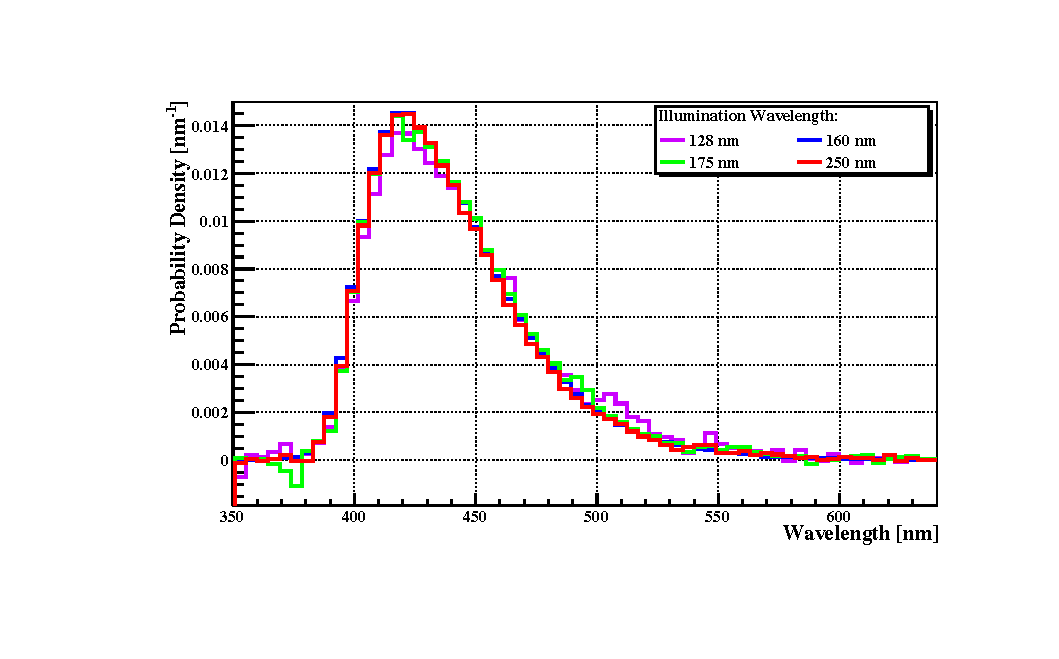
\includegraphics[scale=0.8]{img/TPBSpectrum.pdf}
	
	\caption{\label{fig.tpb} Visible re-emission spectrum for a TPB film illuminated with 128, 160, 175, and 250 nm light. All spectra are normalized to unit area.}
\end{figure}

\begin{figure}[!htb]
	\centering
	\subfloat[Photoelectric event]{
		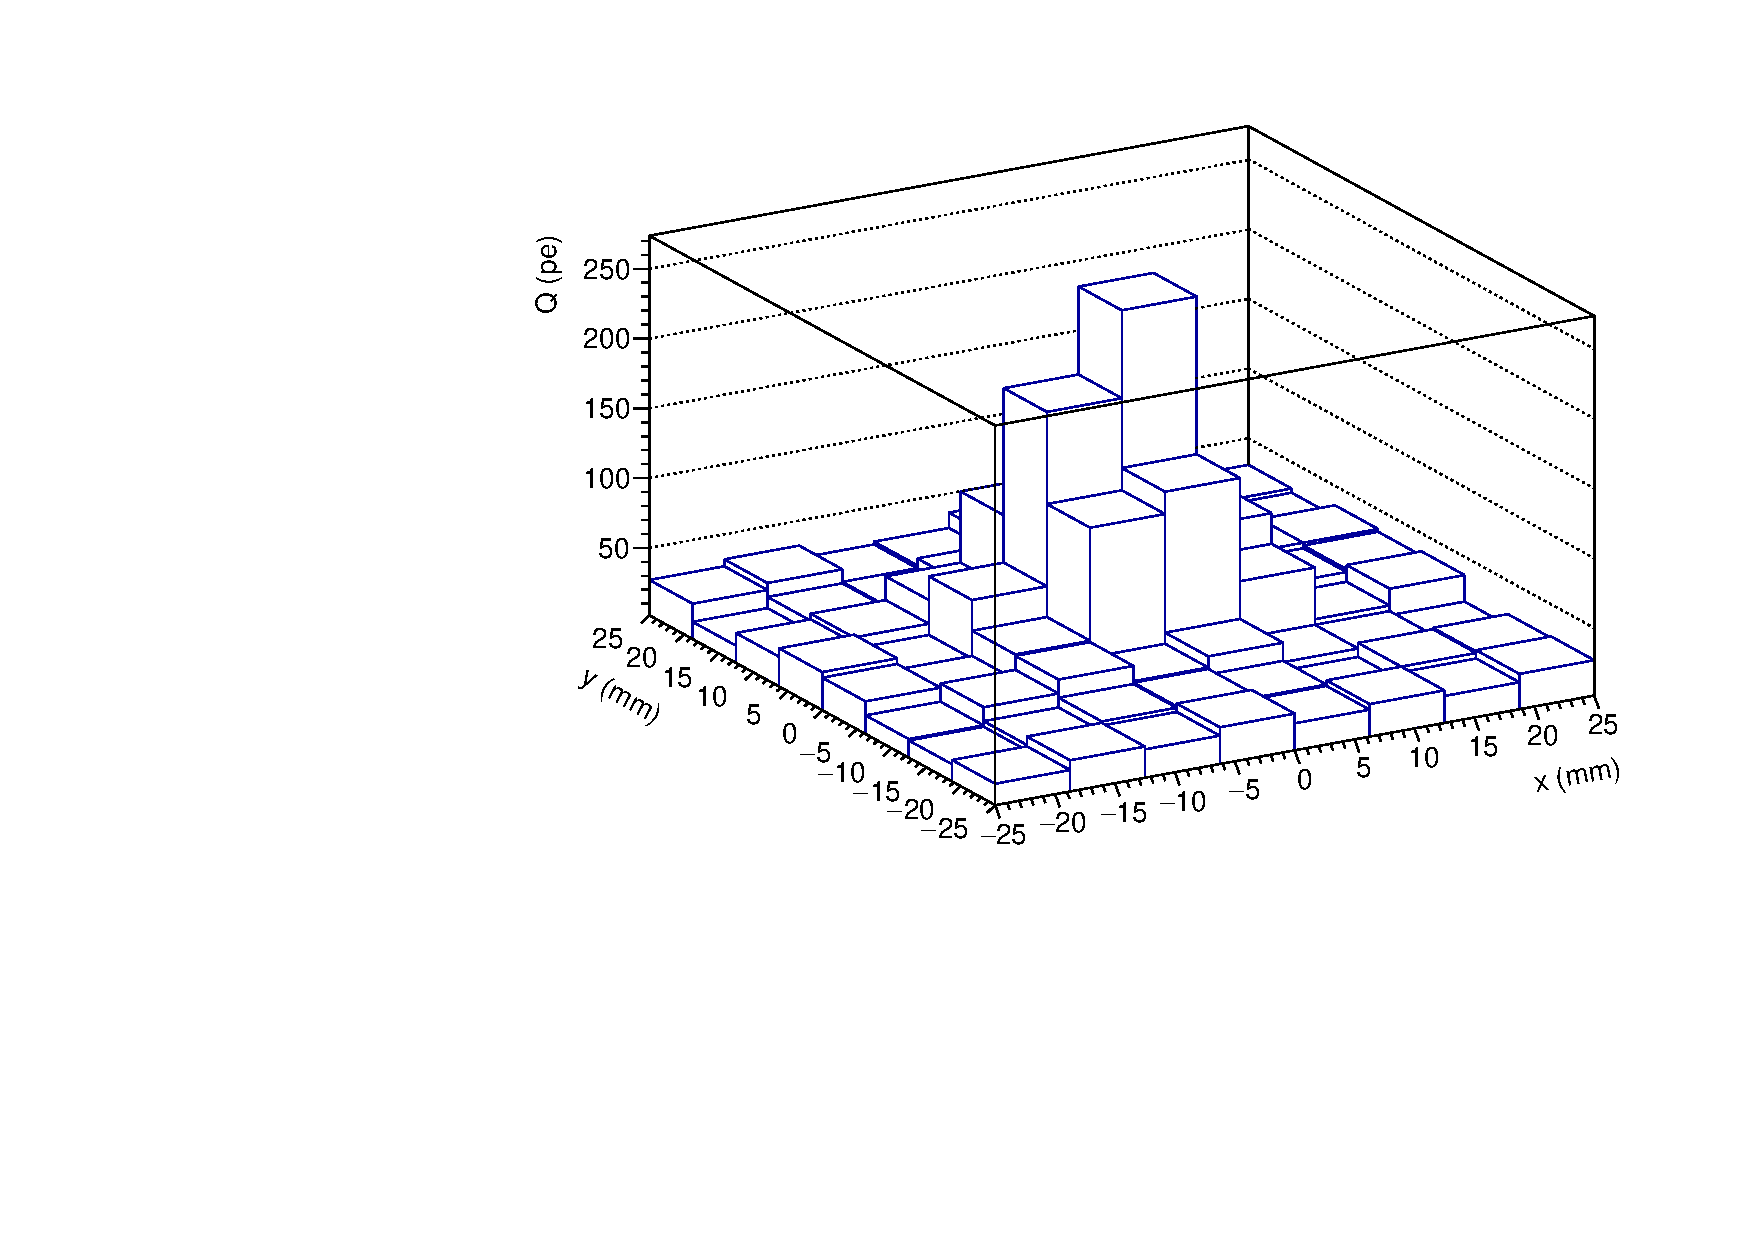
\includegraphics[width=.5\textwidth]{img/photoelectric_in_znear.pdf}
		\label{fig.photoEvent}
	}
	\subfloat[Compton event]{
		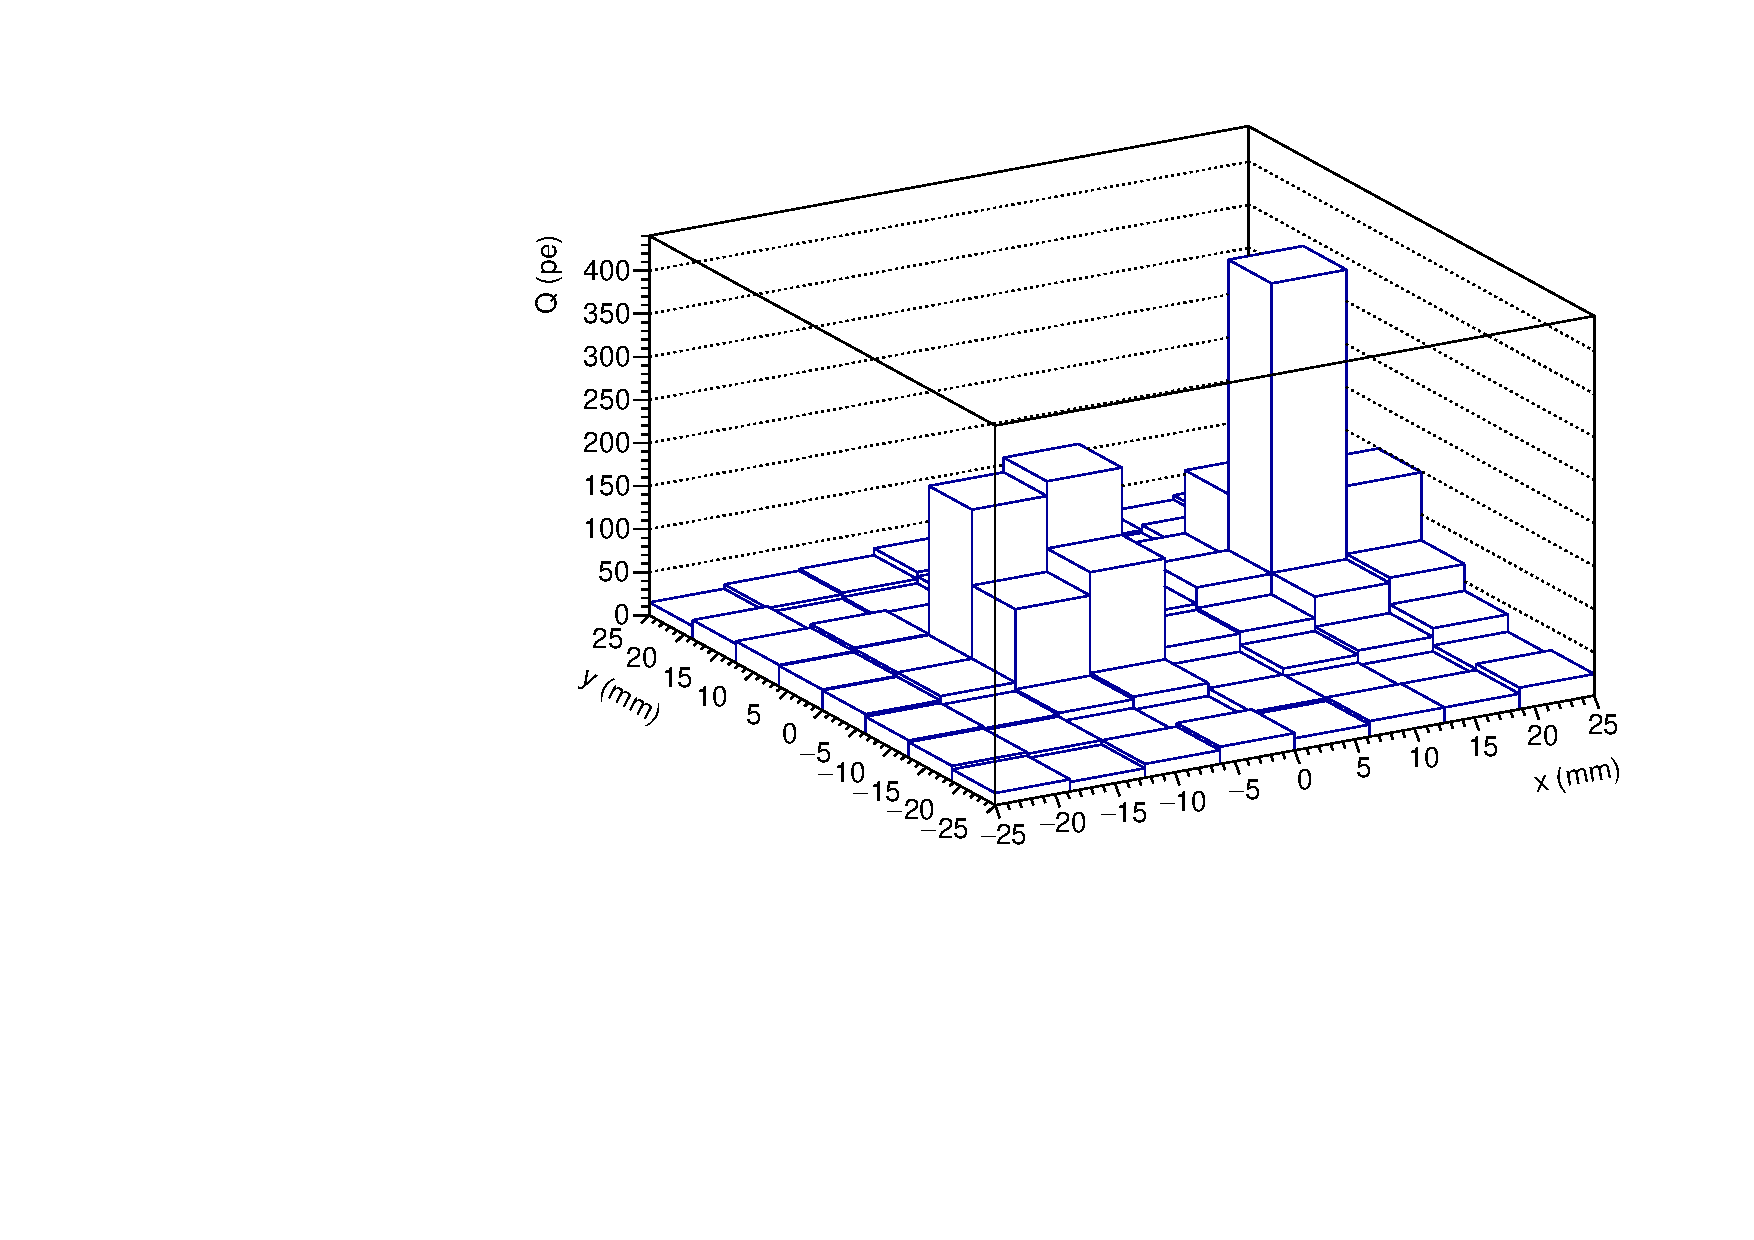
\includegraphics[width=.5\textwidth]{img/compton_2cluster.pdf}
		\label{fig.comptonEvent}
	}
	\caption{\label{fig.events}  Charge on entry plane for two events in the LXSC. (a) Photoelectric event showing a single deposition cluster. (b) Two-site Compton event.}
\end{figure}

A full GEANT4 simulation has been carried out to study the performance of different configurations of the LXSC. Gammas of 511 keV enter the LXSC from outside (defining the ``entry face'') and interact in the cell (see Figure \ref{fig.gammas}), through photoelectric (around 20\% of the times, see Figure \ref{fig.photoEvent}) or Compton interactions (Figure \ref{fig.comptonEvent}). The produced VUV (172 nm) photons are propagated until they hit one of the surfaces of the box. At his point, the effect of the TPB is taking into account. The VUV is absorbed and 80\% of the times (the probability of re-emission, measured by NEXT and other collaborations) a blue photon is emitted isotropically according to the TPB re-emission spectrum measured by the NEXT collaboration and shown in Figure \ref{fig.tpb}.

The emitted photon can then impinge on a SiPM, in which case a signal is generated in the SiPM with a probability following the PDE probability distribution shown in Figure \ref{fig.pde}. At this point, one can add the noise due to DCR, optical cross talk, etc. However, the noise due to DCR is sufficiently small at the LXe temperatures as to be negligible. For this studies we have not included yet the effect of optical cross-talk, which are very dependent of the specific SiPM model used for the LXSC and will, in any case, be small.  

%
%%1314_2planes_100000.root , energyDist.c
%\begin{figure}[!htb]
%	\begin{center}
%           \subfloat[XY distribution]{
%               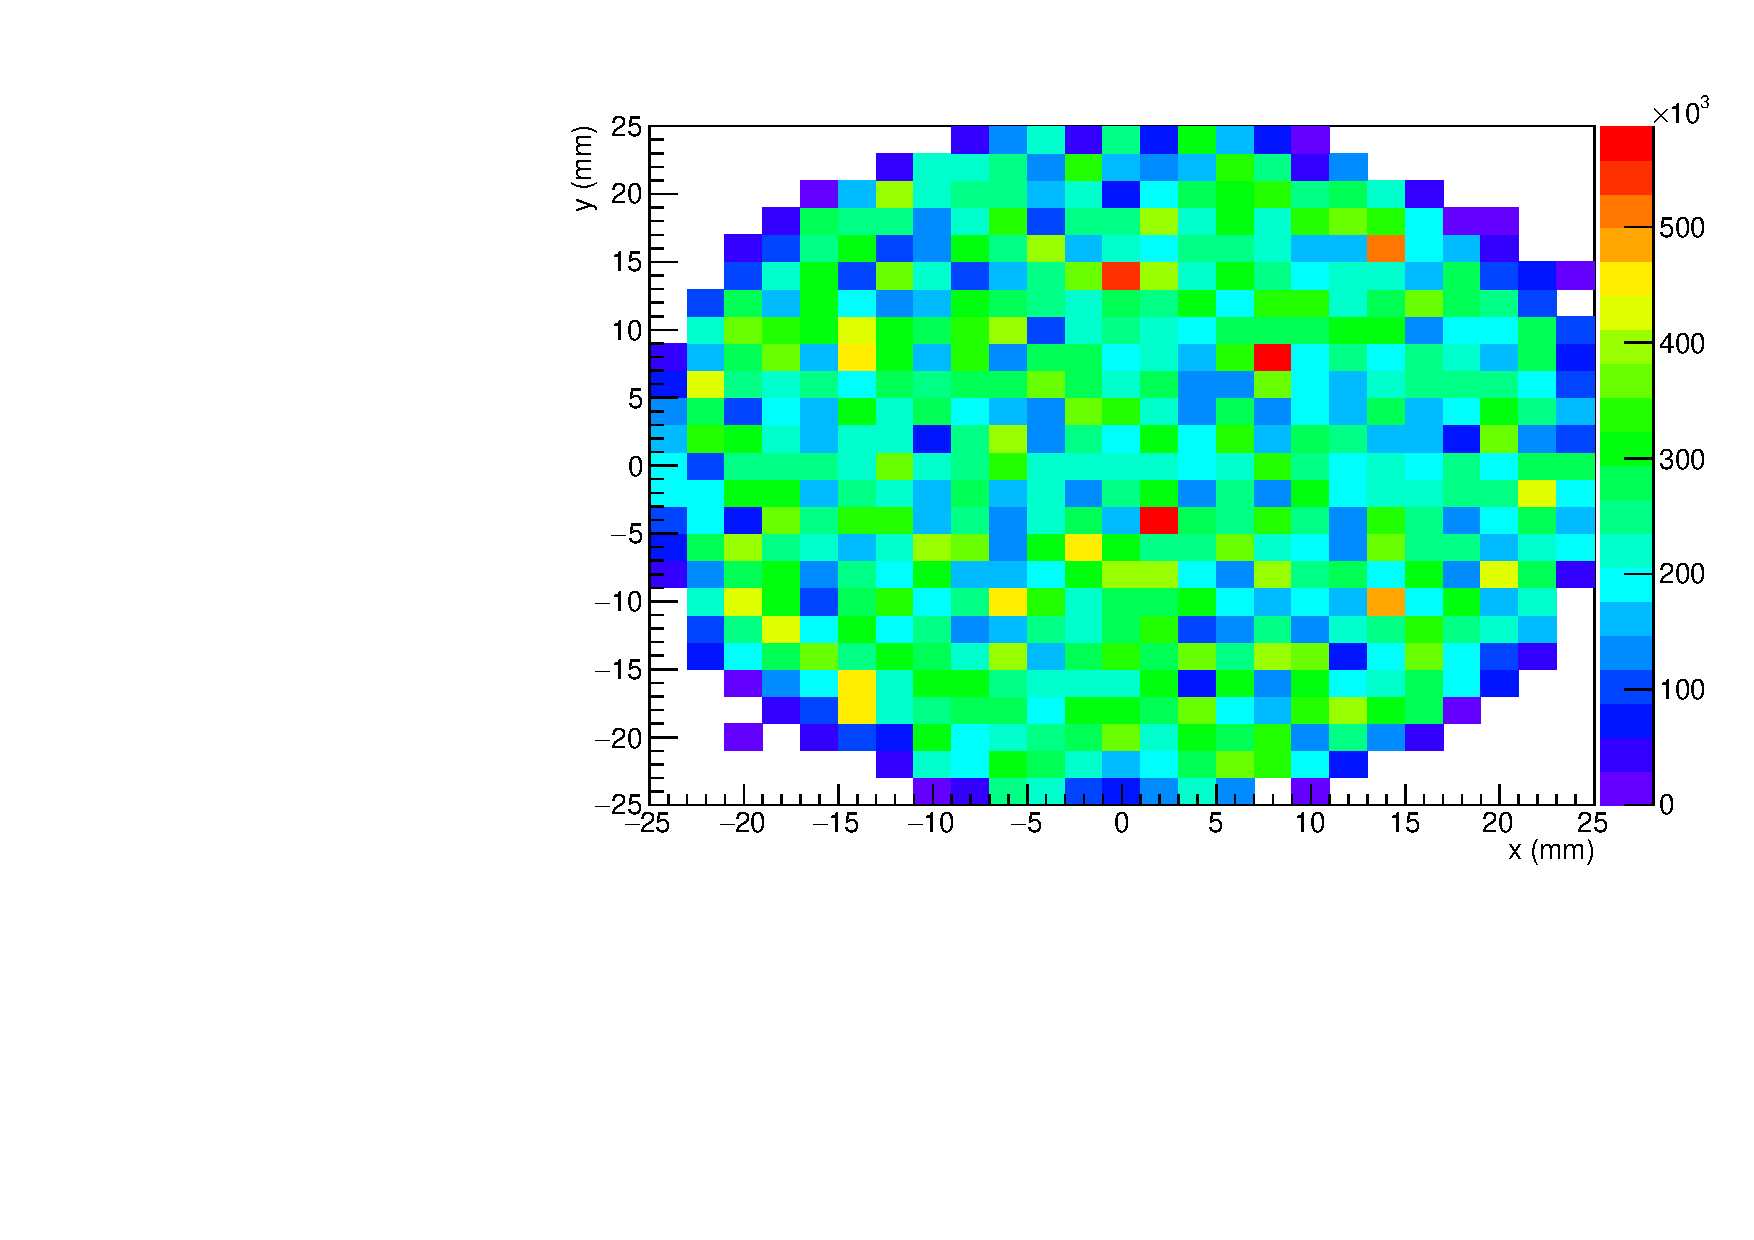
\includegraphics[width=.5\textwidth]{img/energyXY.pdf}
%           }
%           \subfloat[XZ distribution]{
%               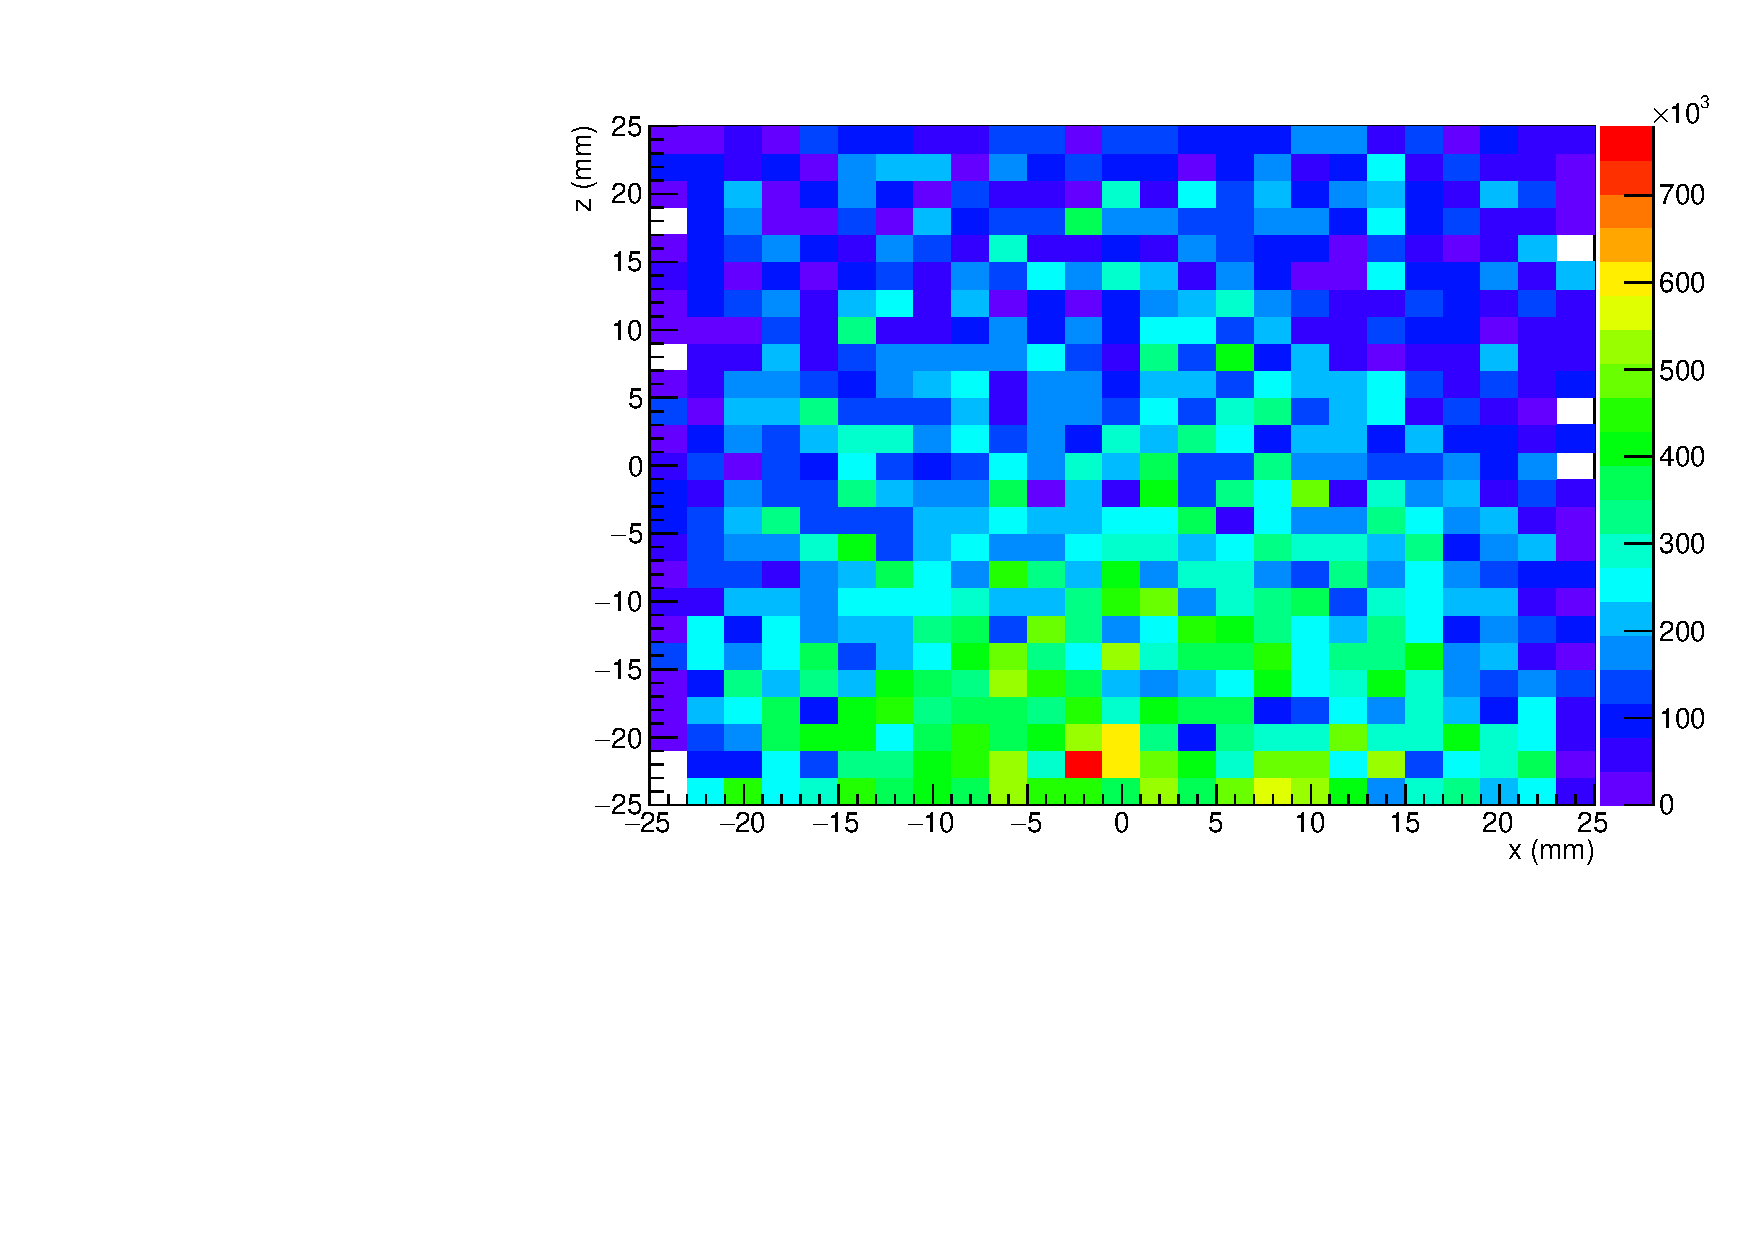
\includegraphics[width=.5\textwidth]{img/energyXZ.pdf}
%           }
%           \caption{\label{fig.gammas} Gamma generation from outside the box using solid angle. (a) X,Y distribution of the gammas interacting in the LXSC. (b) X,Z distribution, showing an accumulation of interactions in the first 3 cm.  }
%    \end{center}
%\end{figure}



%In order to inspect possible edge effects in the LXSC we have also run simulations changing the generation of the gammas, instead of being fired from the outside of the box within a solid angle, they start at a random point of the entry plane of the box. In this way we have events in every part of the box (see Figure \ref{fig.distNewgen}). In any case we have seen this change does not affects energy or spatial resolutions. 
%Despite of that, given the fact that algorithms to reconstruct Compton interactions are sensitive to the incoming direction we will keep generating gammas outside the box.

%lxsc2_z5.root , energyDistNewGen.c
\begin{figure}[!htb]
        \begin{center}
                \subfloat[XY distribution]{
                        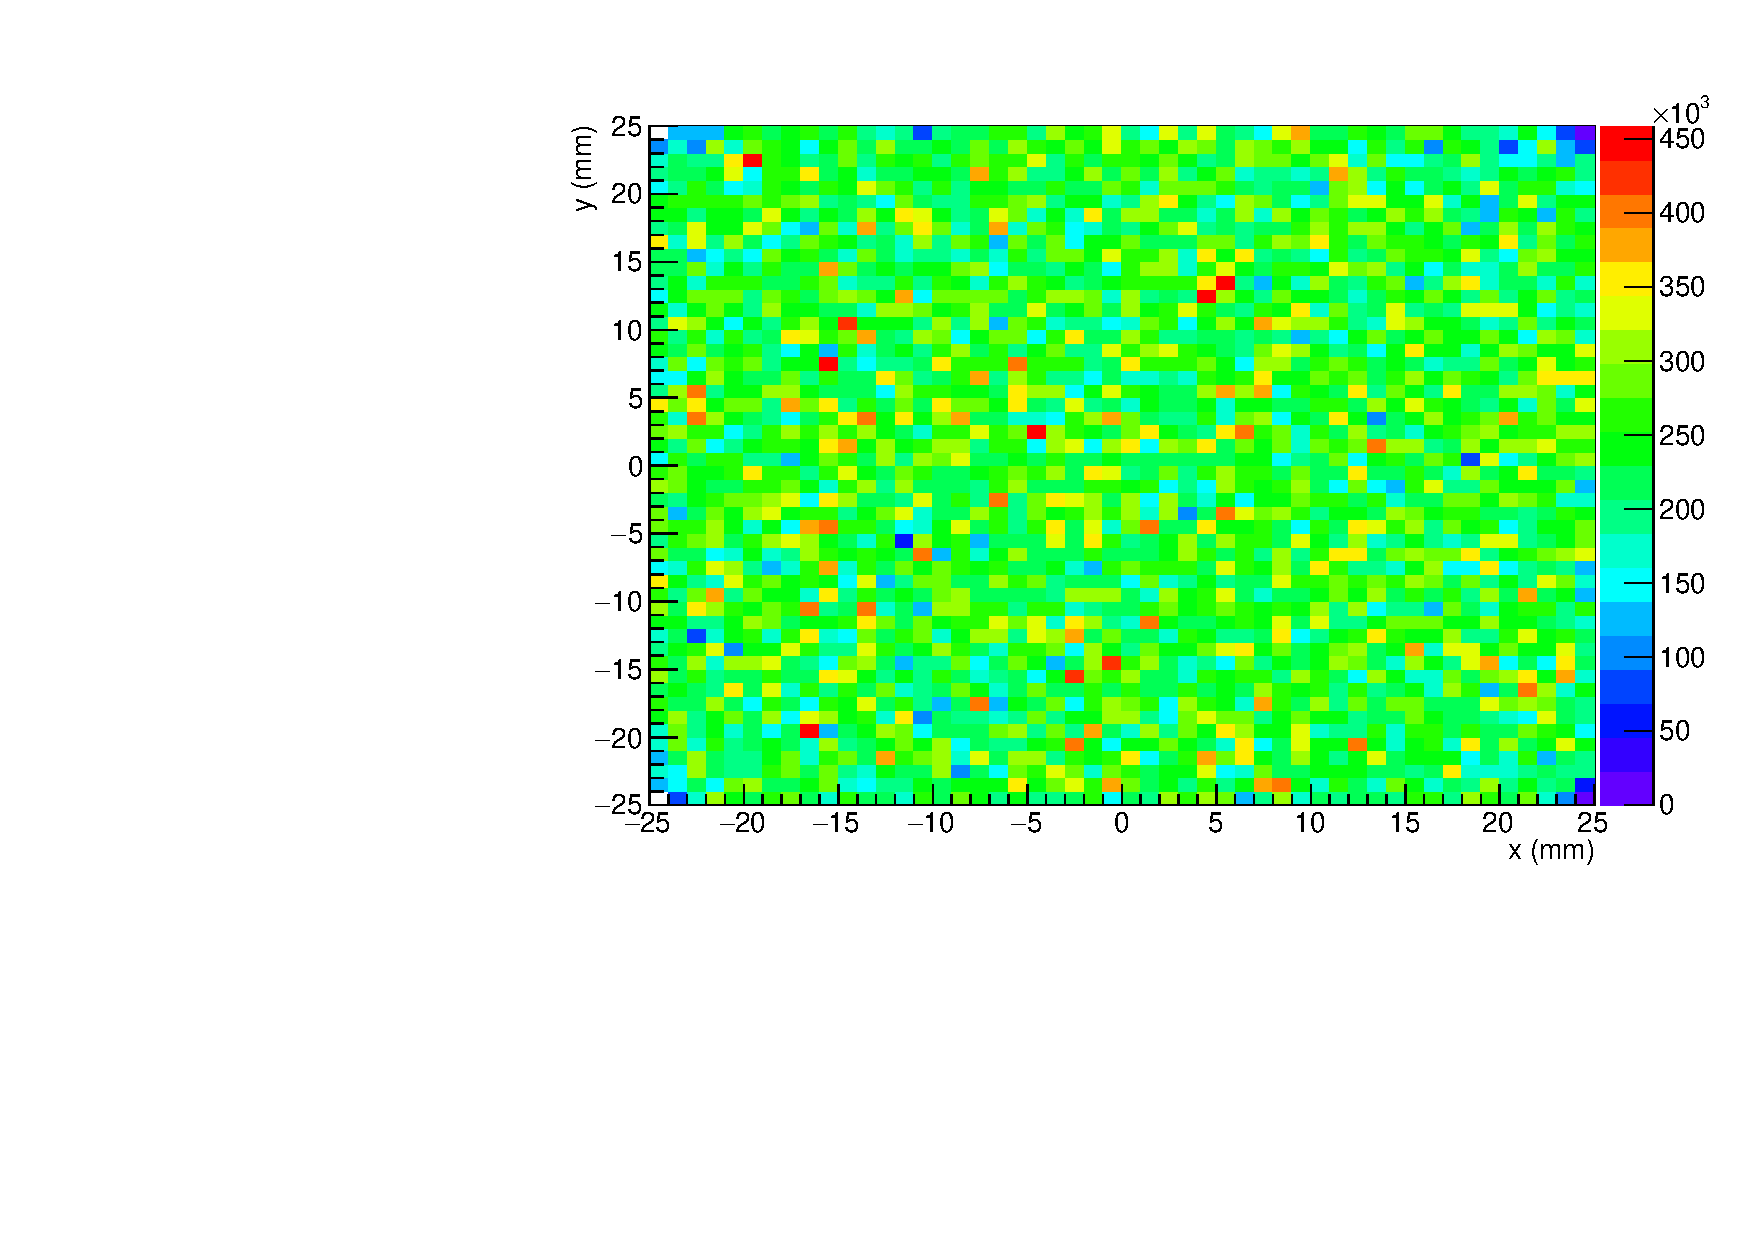
\includegraphics[width=.5\textwidth]{img/energyXY_newgen.pdf}
                }
                \subfloat[XZ distribution]{
                        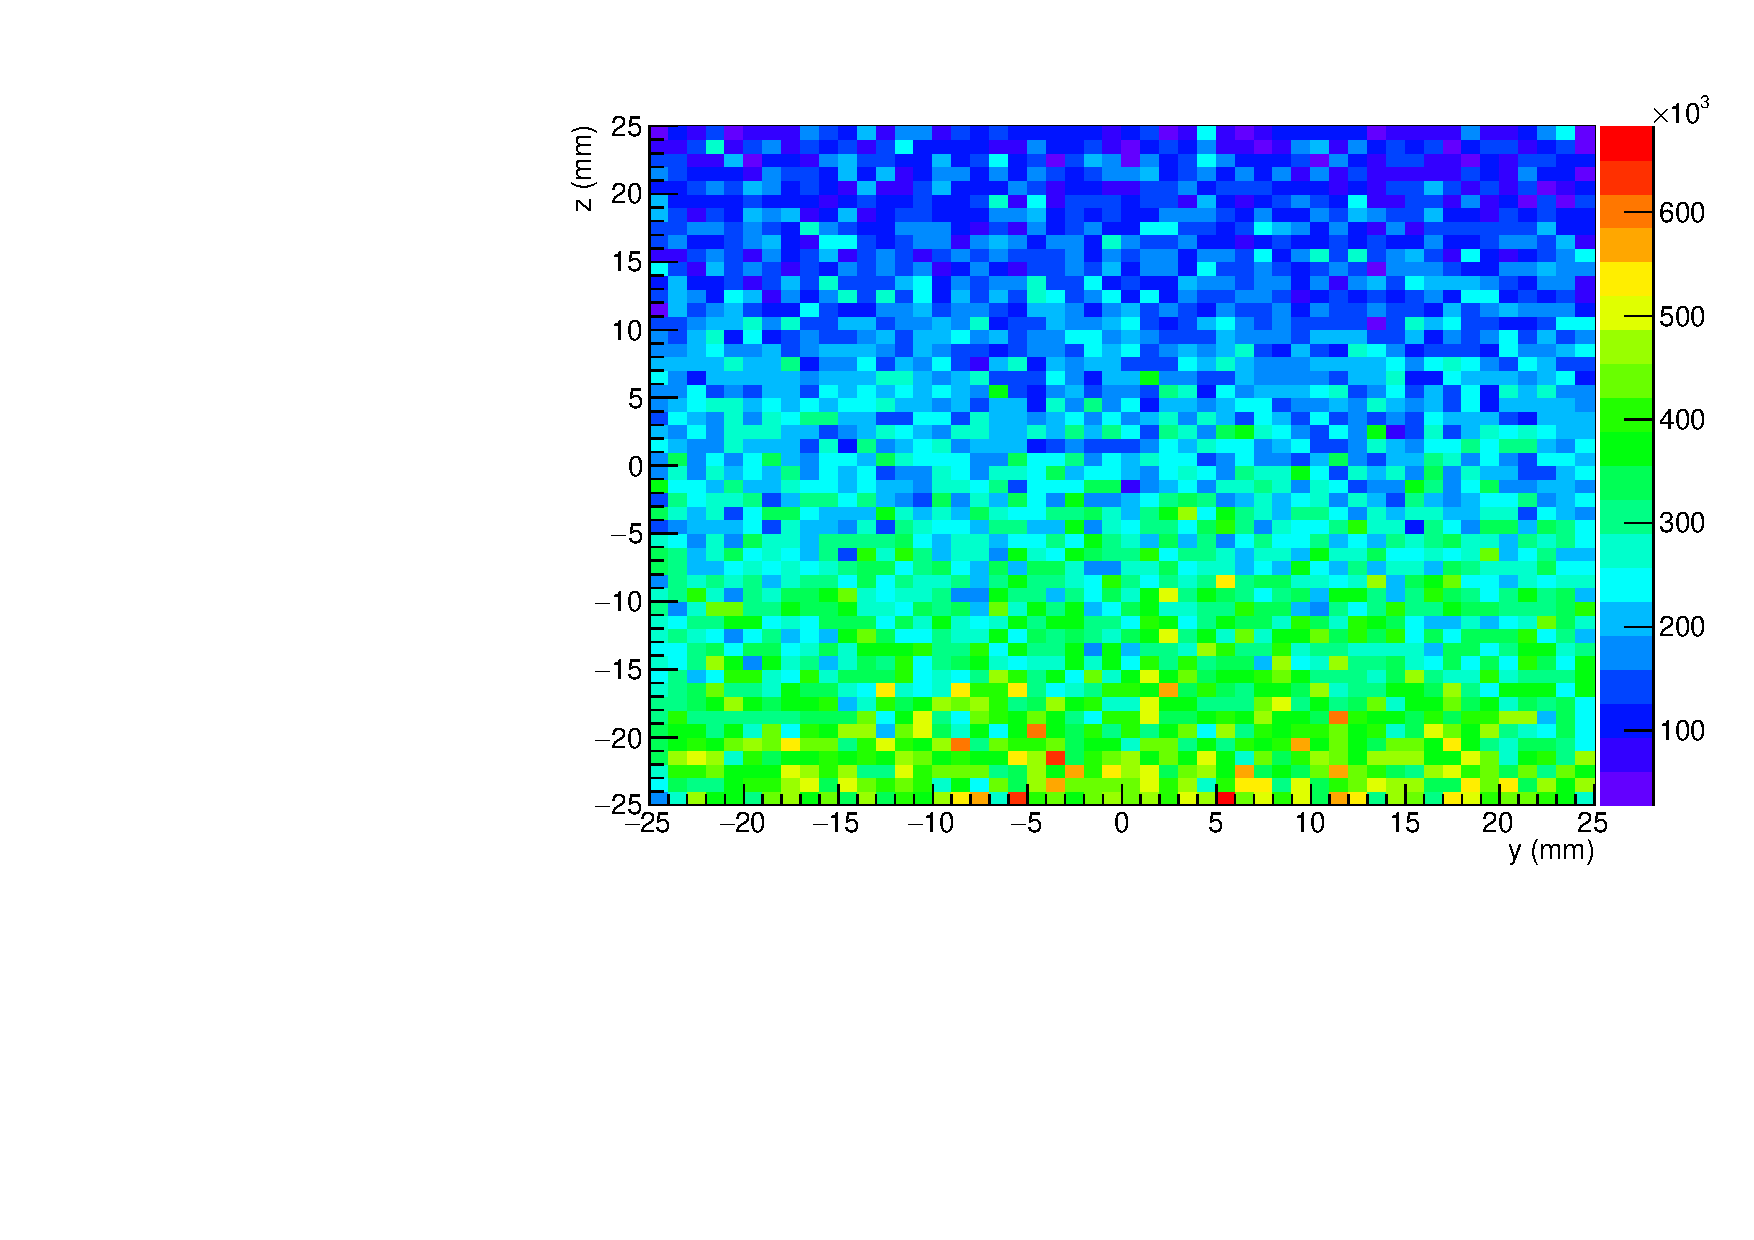
\includegraphics[width=.5\textwidth]{img/energyXZ_newgen.pdf}
                }
                \caption{\label{fig.distNewgen} (a) X,Y distribution of the gammas interacting in the LXSC. (b) X,Z distribution, showing an accumulation of interactions in the first 3 cm  as expected from the attenuation length.}
        \end{center}
\end{figure}

 Figure \ref{fig.distNewgen} shows the distribution of gammas generated in a specific run, distributed uniformly along x-y (transverse coordinates) and shot at $z=0$. Notice that the interactions accumulate in the firs 3 cm of the cell, as expected from the attenuation length.  
 
 \subsection{Configurations of the LXSC}

\begin{figure}[!htb]
	\centering
	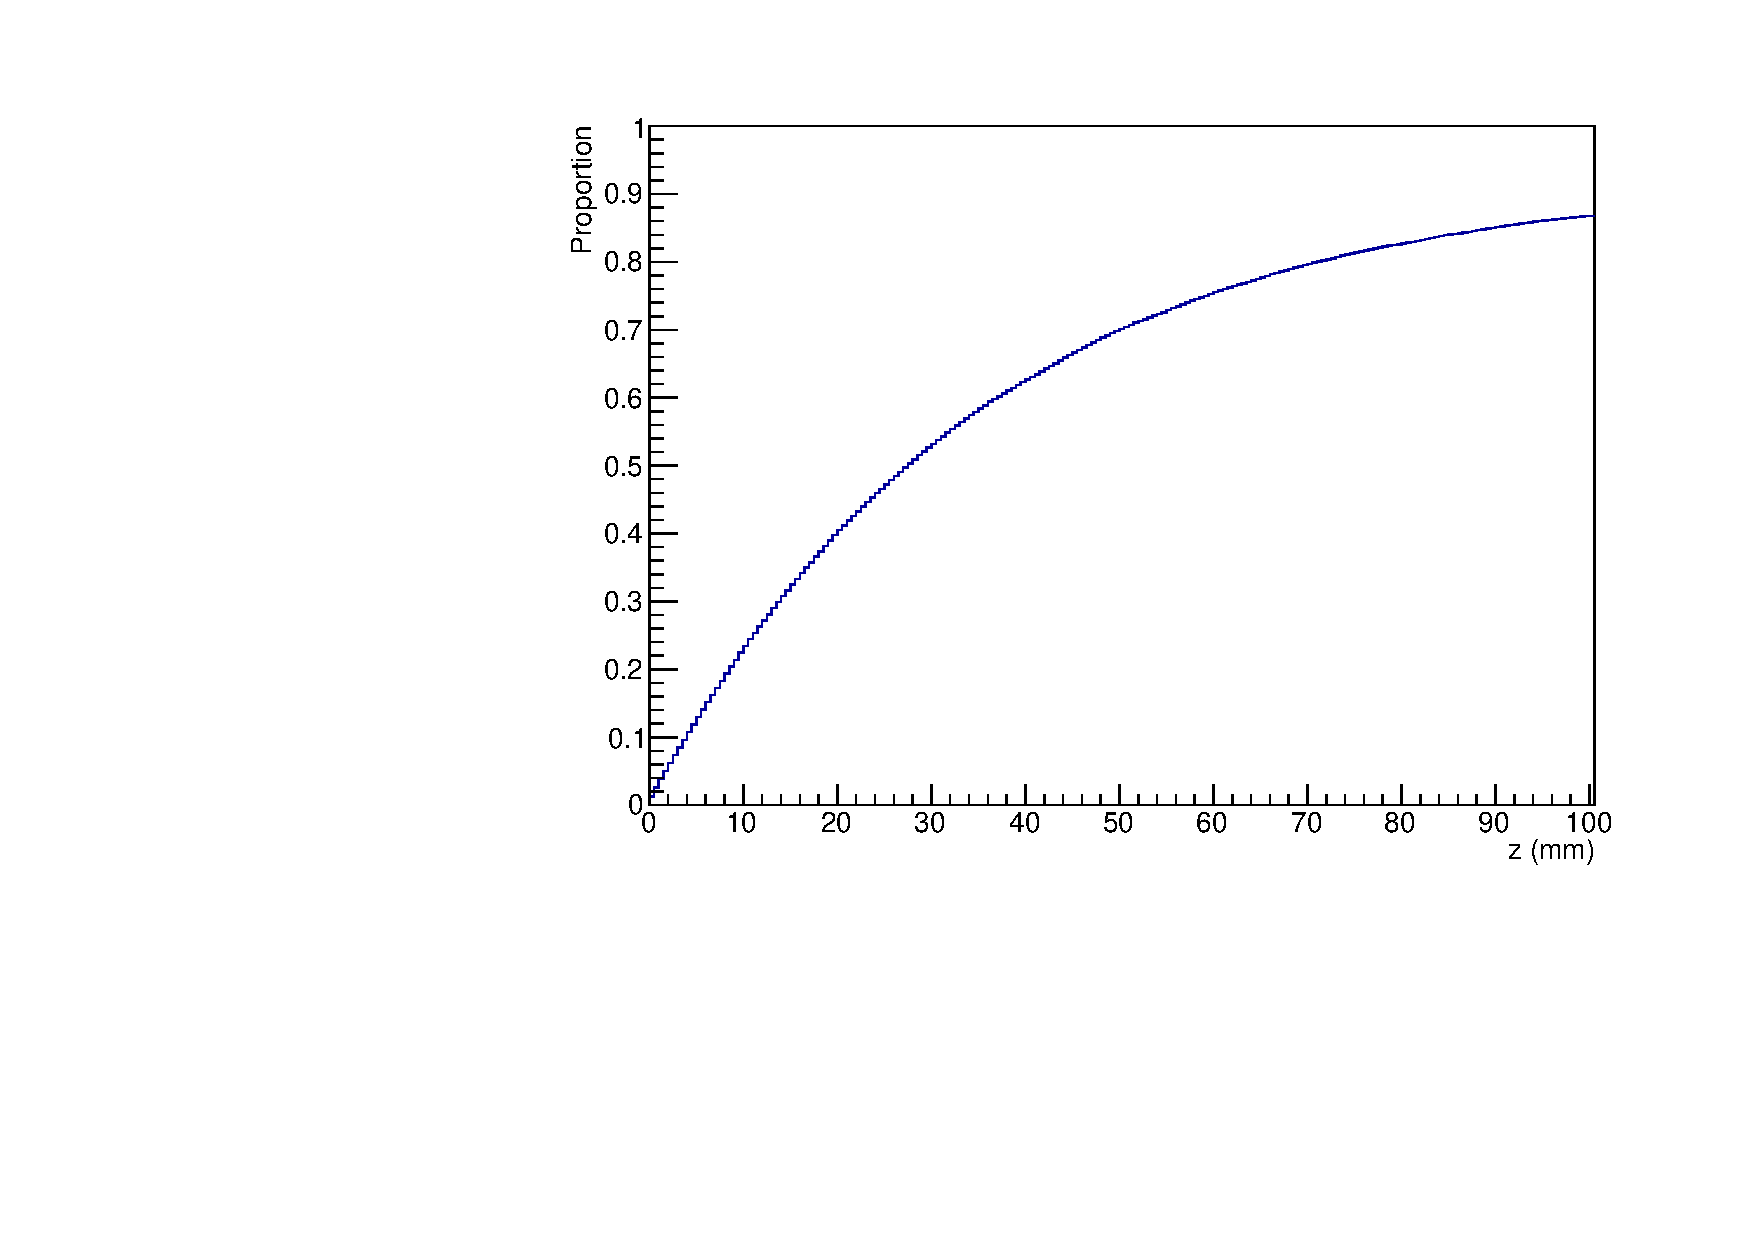
\includegraphics[scale=0.5]{img/zProportion.pdf}
	\caption{\label{fig.proportion} Proportion of events in function of position in $z$ coordinate. With 5 cm approximately $77\%$ of the incoming gammas interact in the active volume of the detector.}
\end{figure}


The geometry and instrumentation of the LXSC can be tuned up depending on the intended application. The most important parameters to be varied are: 
\begin{enumerate}
\item {\bf Shape and transverse dimensions}: The simplest design of the LXSC is a simple box, but other geometries, such as a trapezoid (a truncated pyramid) may be more suitable for packing the modules in a PET ring. The transverse dimensions can also be tuned up depending on the packing needs (e.g, the size of the ring). The default chosen for most of our studies for the LXSC is a box of $5 \times 5$~cm$^2$~transverse size.
\item {\bf Thickness}: our default (5 cm) represents a compromise between the conflicting requirements of good efficiency (which improves with thickness) and good spatial resolution (which worsens with thickness). With 5 cm thickness 77\% of the impending 511 keV gammas interact in the cell  (see Figure \ref{fig.proportion}).
\item {\bf Number of instrumented faces}: The best performance is obtained when all the faces are instrumented, maximizing light collection (thus energy resolution) and minimizing inhomogeneities (thus improving energy resolution and spatial resolution). On the other hand, such an arrangement is too expensive, as well as impractical for packing (e.g, arranging the boxes into a ring) purposes. Alternative configurations can instrument 4 or even 2 planes, which result, indeed, in the best overall compromise. 
\item {\bf Number of SiPMs per face}: again, the best response is achieved when the faces are fully covered by SiPMs, but in more sparse configuration reduced cost can be traded by performance.
\end{enumerate}

%In this study we have simulated a box of $5\times5\times5$ cm$^3$~with the following configurations: 
%
%\begin{itemize}
%\item \textbf{LXSC2-36}:  $6\times6$ SiPM on two planes (entry and exit).
%\item \textbf{LXSC2-49}:  $7\times7$ SiPM on two planes (entry and exit).
%\item \textbf{LXSC2-64}:  $8\times8$ SiPM on two planes (entry and exit).
%
%\item \textbf{LXSC4-36}:  $6\times6$ SiPM on four planes (entry, exit and two parallel sides).
%\item \textbf{LXSC4-49}:  $7\times7$ SiPM on four planes (entry, exit and two parallel sides).
%\item \textbf{LXSC4-64}:  $8\times8$ SiPM on four planes (entry, exit and two parallel sides).
%
%\item \textbf{LXSC6-36}:  $6\times6$ SiPM on six planes.
%\item \textbf{LXSC6-49}:  $7\times7$ SiPM on six planes.
%\item \textbf{LXSC6-64}:  $8\times8$ SiPM on six planes.
%\end{itemize}
%
%On the other hand, as discussed above, the spatial resolution depends of the box thickness. The response of the SiPMs is sharper when the interactions take place near some of the instrumented planes, and therefore, a thinner box results in better spatial resolution. On the other hand, as we reduce the thickness, the detection efficiency decreases.  To study this size-resolution trade-off we have run simulations with the following configurations:
%
%\begin{itemize}
%\item \textbf{LXSC2-Z2}:  $5\times5\times2$ cm$^3$ box with $8\times8$ SiPM on two planes (entry and exit).
%\item \textbf{LXSC2-Z3}:  $5\times5\times3$ cm$^3$ box with $8\times8$ SiPM on two planes (entry and exit).
%\item \textbf{LXSC2-Z4}:  $5\times5\times4$ cm$^3$ box with $8\times8$ SiPM on two planes (entry and exit).
%\item \textbf{LXSC2-Z5}:  $5\times5\times5$ cm$^3$ box with $8\times8$ SiPM on two planes (entry and exit).
%\end{itemize}

%After analyzing those, there is some improvement in spatial resolution (see Section \ref{sec.spatial}) but a lot of incoming gammas are lost (see Table \ref{tab.lxscZ}), making it clear that we should not have less than 5 cm in the longitudinal coordinate. The fractions shows in Table \ref{tab.lxscZ} includes only those interacting the active volume of the detector, there is a small fraction of gammas interacting in the walls of the detector that are not included.

%\begin{table}[h]
%\caption{\label{tab.lxscZ}Number of 511 keV gammas interacting in LXSC for different longitudinal sizes.}
%\begin{center}
% \begin{tabular}{c|ccc}
%  \toprule
%   \textbf{Longitudinal size} & \textbf{$\gamma$ simulated} & \textbf{Interactions} & \textbf{Fraction} \\
%   \hline
%  {\bf 2 cm} & 500000 & 207047 & 41.4 \% \\
%  {\bf 3 cm} & 500000 & 270172 & 54.0 \% \\
%  {\bf 4 cm} & 500000 & 318649 & 63.7 \% \\
%  {\bf 5 cm} & 500000 & 355536 & 71.7 \% \\
%  \toprule
% \end{tabular}
%\end{center}
%\end{table}
%

%\newpage
%\thispagestyle{newstyle}
\subsection{Energy resolution of the LXSC}
\label{sec.energy}

%The VUV photons produced by the interactions of gammas in the LXSC are shifted to 420 nm by the TPB which coats the teflon panels and the SiPMs. The conversion efficiency, measured, among other authors by the NEXT collaboration is 80\%. The resulting blue photons are registered by the SiPMs, with high efficiency (the typical PDE of modern SiPMs for 420 nm exceeds 50\%. For this specific study we have simulated the 6 mm SENSL C-series sensor). 
%
%While the fast decay time of scintillation (2 ns) allows for TOF applications (see Section \ref{sec.tof}), the longer time associated with the recombination of electrons (45 ns) implies integration times of the order of 200-300 ns, similar to those used by LSO detectors. The dark current of the SiPMs and the electronic noise of the front-end electronics (in the case than an ASIC is used) is very low due to the cryogenic operation, and thus the resolution is dominated by photoelectron statistics. 

\begin{figure}[!htb]
	\centering
	\subfloat[LXSC6-64]{
		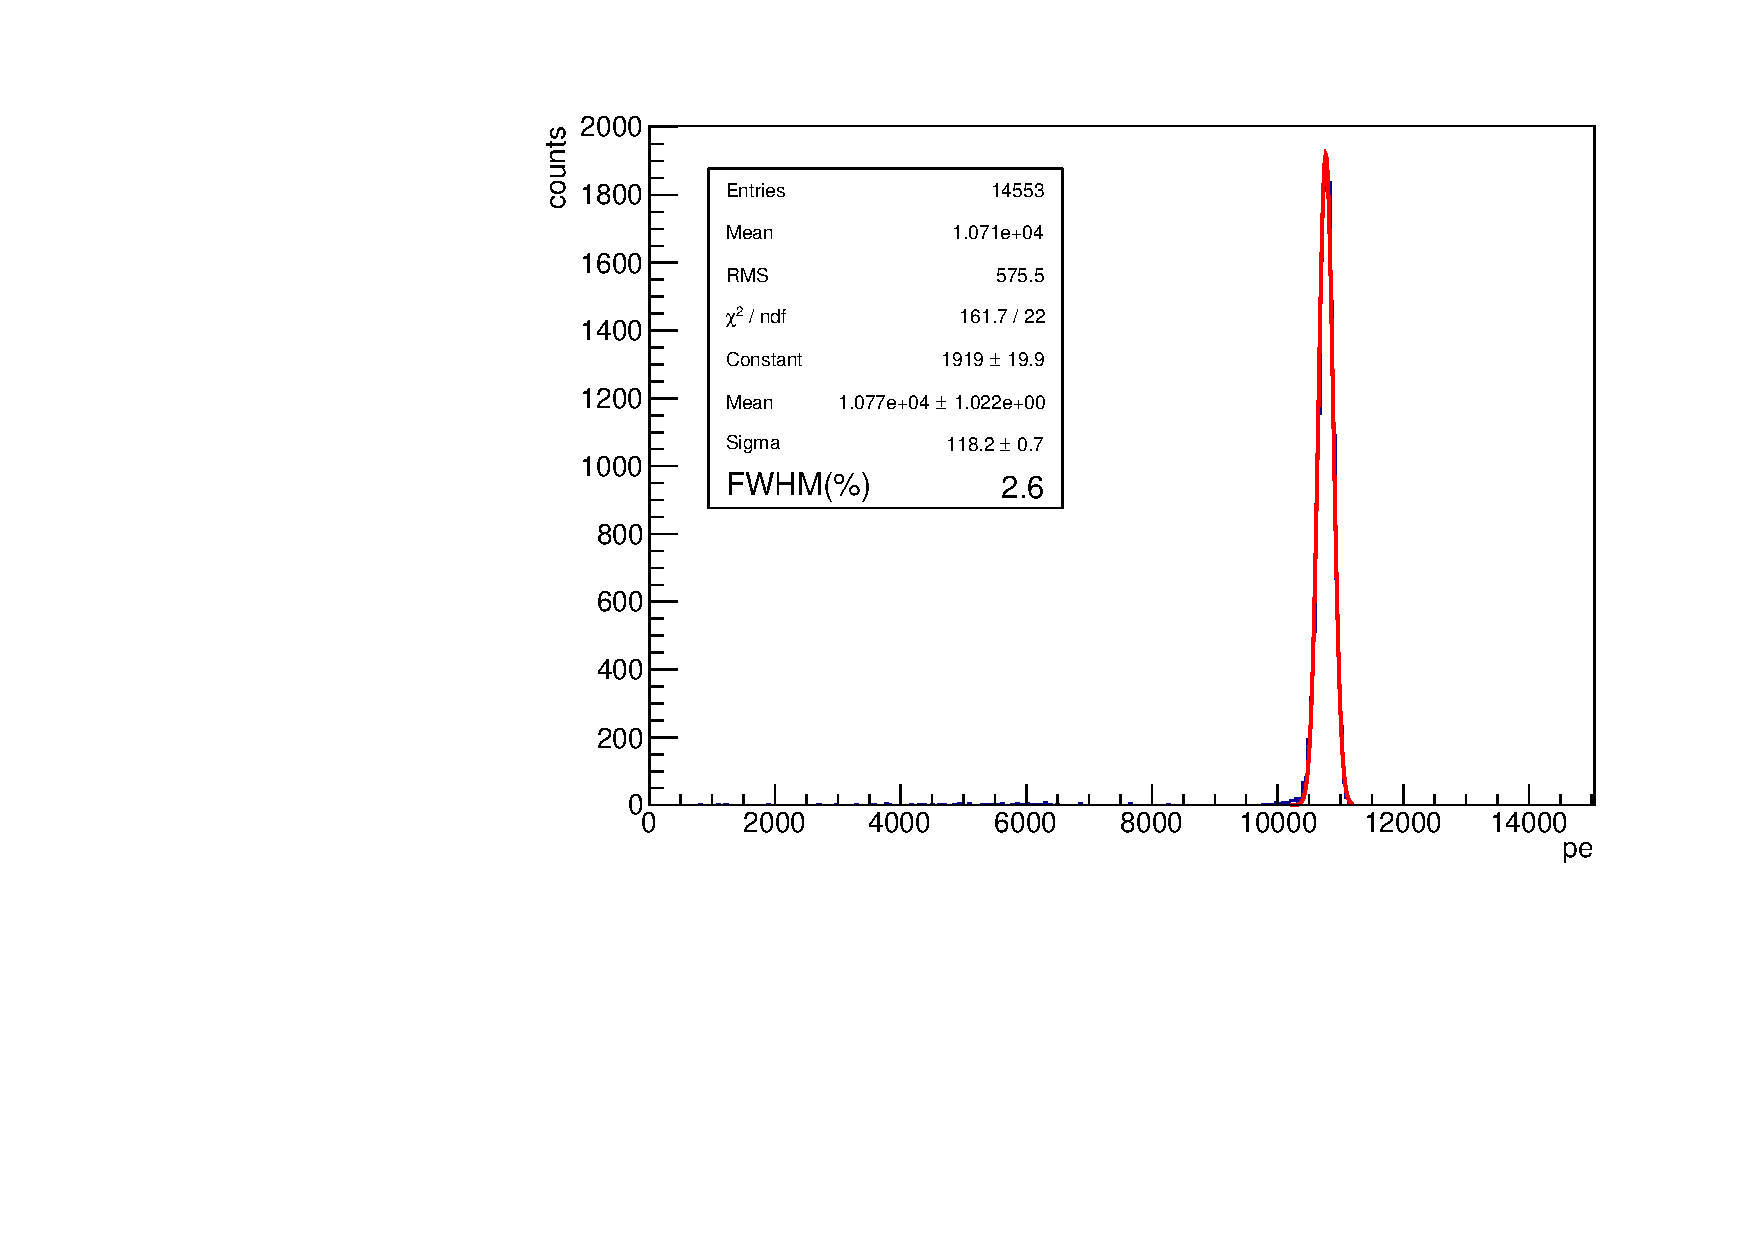
\includegraphics[width=.55\textwidth]{img/energy_6_64.pdf}
		\label{fig.energy664}
	}
	\subfloat[LXSC2-36]{
		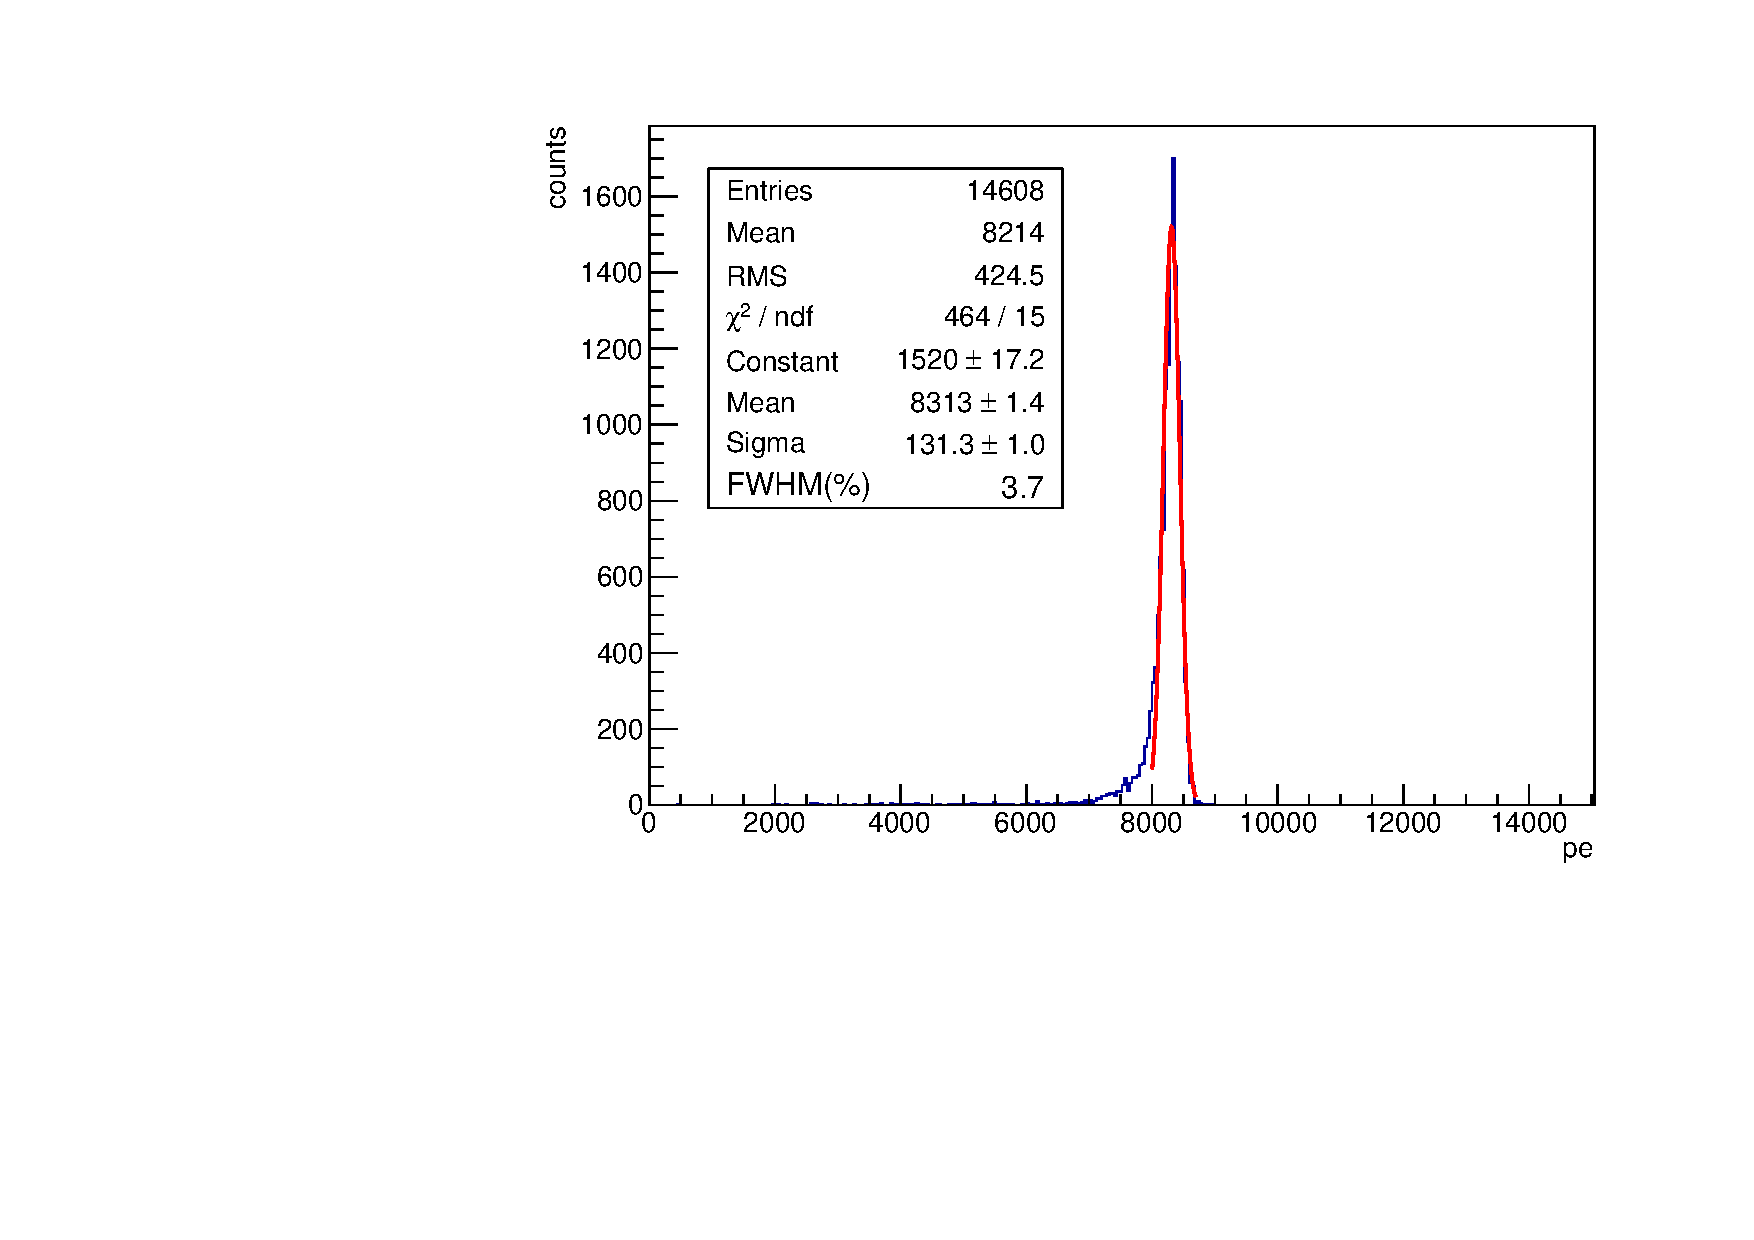
\includegraphics[width=.55\textwidth]{img/energy_2_36.pdf}
		\label{fig.energy236}
	}
	\caption{\label{fig.energy} (a) The intrinsic energy resolution of the LXSC6 is excellent (2.6\% FWHM) due to the high photoelectron statistics. (b) The most sparse configuration, LXSC2 records less light, but the resolution is still very good (3.7\% FWHM).}
\end{figure}

Figure \ref{fig.energy664} shows the recorded number of photoelectrons in the LXSC6-64 corresponding to photoelectric interactions. The fit shows a resolution of 2.6\% FWHM, {\em much better} than the resolution obtained with conventional SSDs (for example, the best resolution obtained with test systems for LSO crystals is in the vicinity of 9 \% FWHM, while commercial PETs typically show a resolution of around 20 \% FWHM). Figure \ref{fig.energy236} shows the recorded number of photoelectrons in the LXSC2-36 corresponding to photoelectric interactions ($\sim$ 8000 P.E., to be compared with $\sim$ 11000 P.E. for the LXSC6). The  fit yields a resolution of 3.7\% FWHM. This is still very good, but it can be further improved by applying geometrical corrections.

\begin{figure}[!htb]
	\centering
			\subfloat[LXSC6, $x$ coordinate]{
				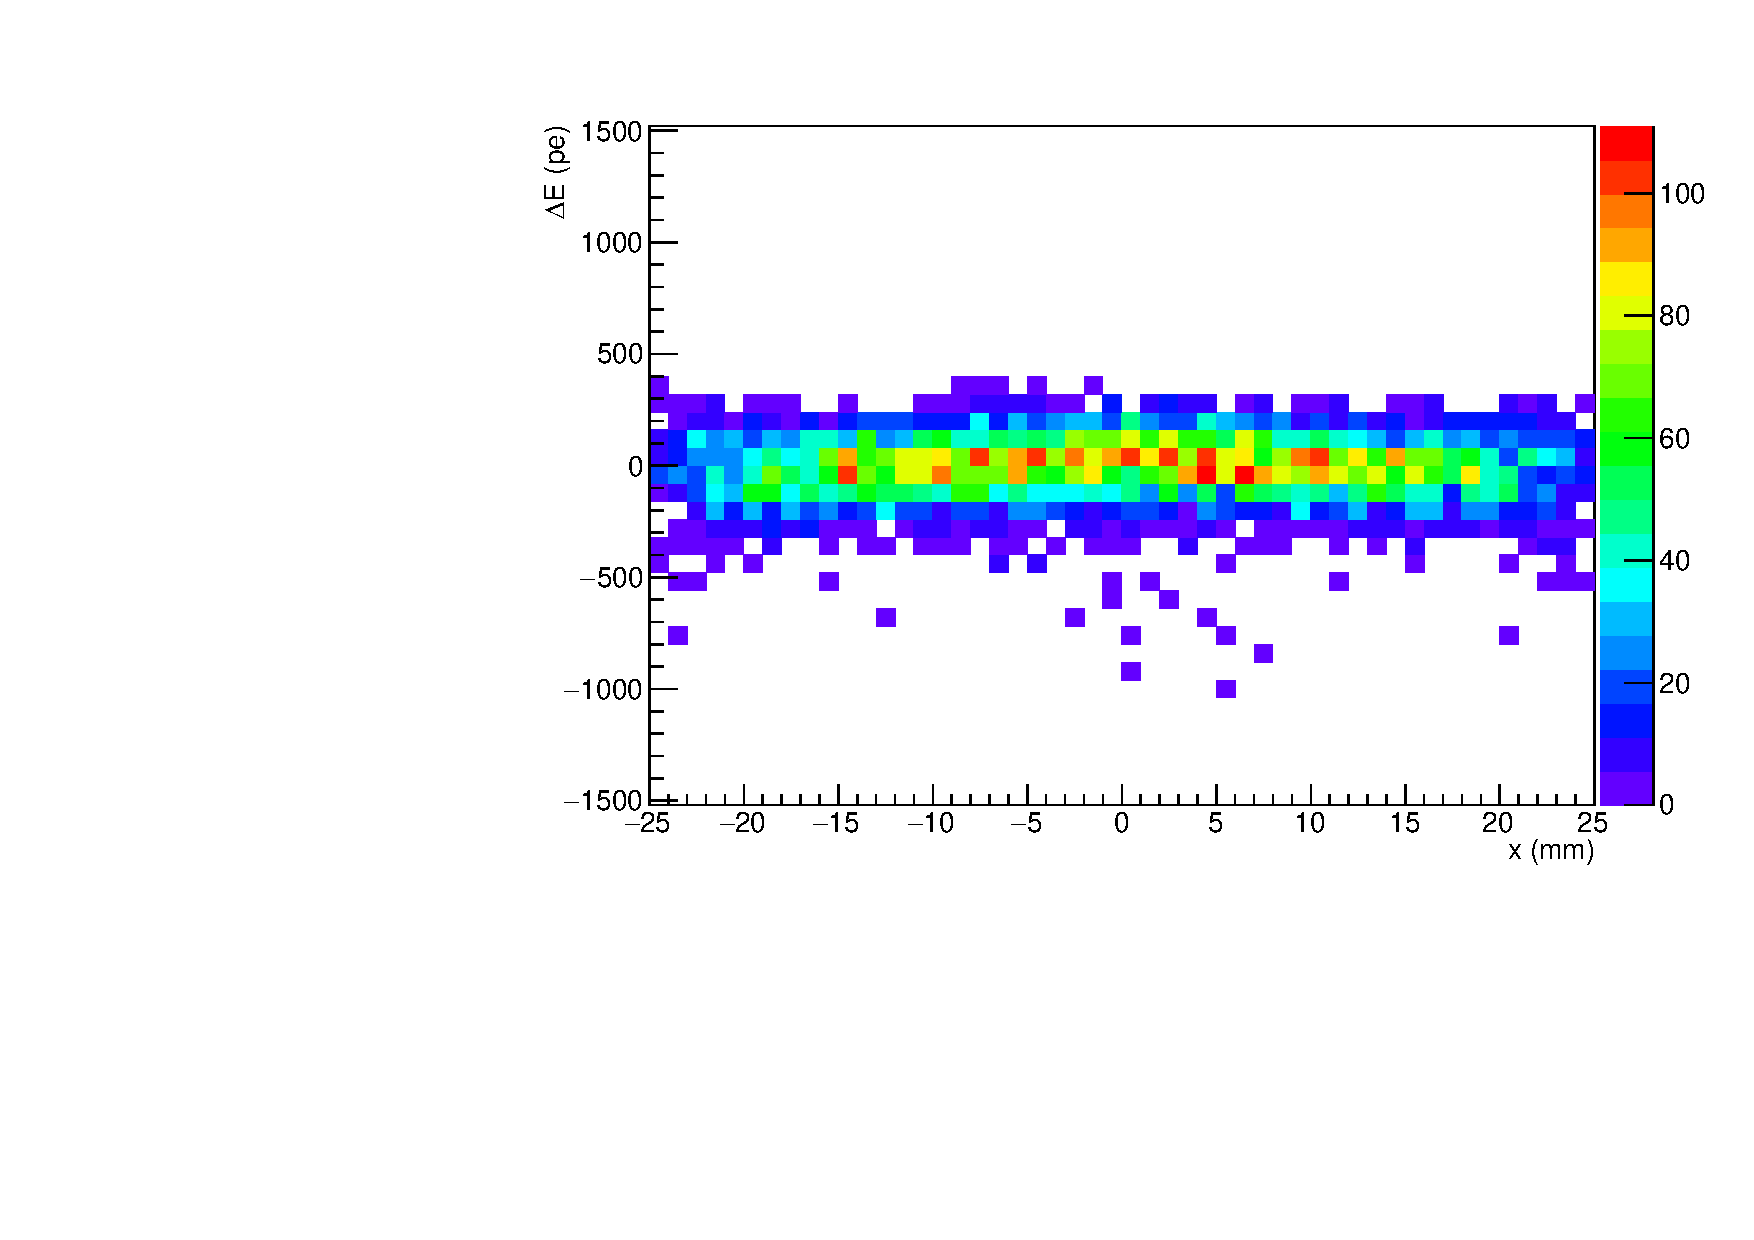
\includegraphics[width=.5\textwidth]{img/eposx_664.pdf}
				\label{fig.eposx664}
			}
			\subfloat[LXSC6, $z$ coordinate]{
				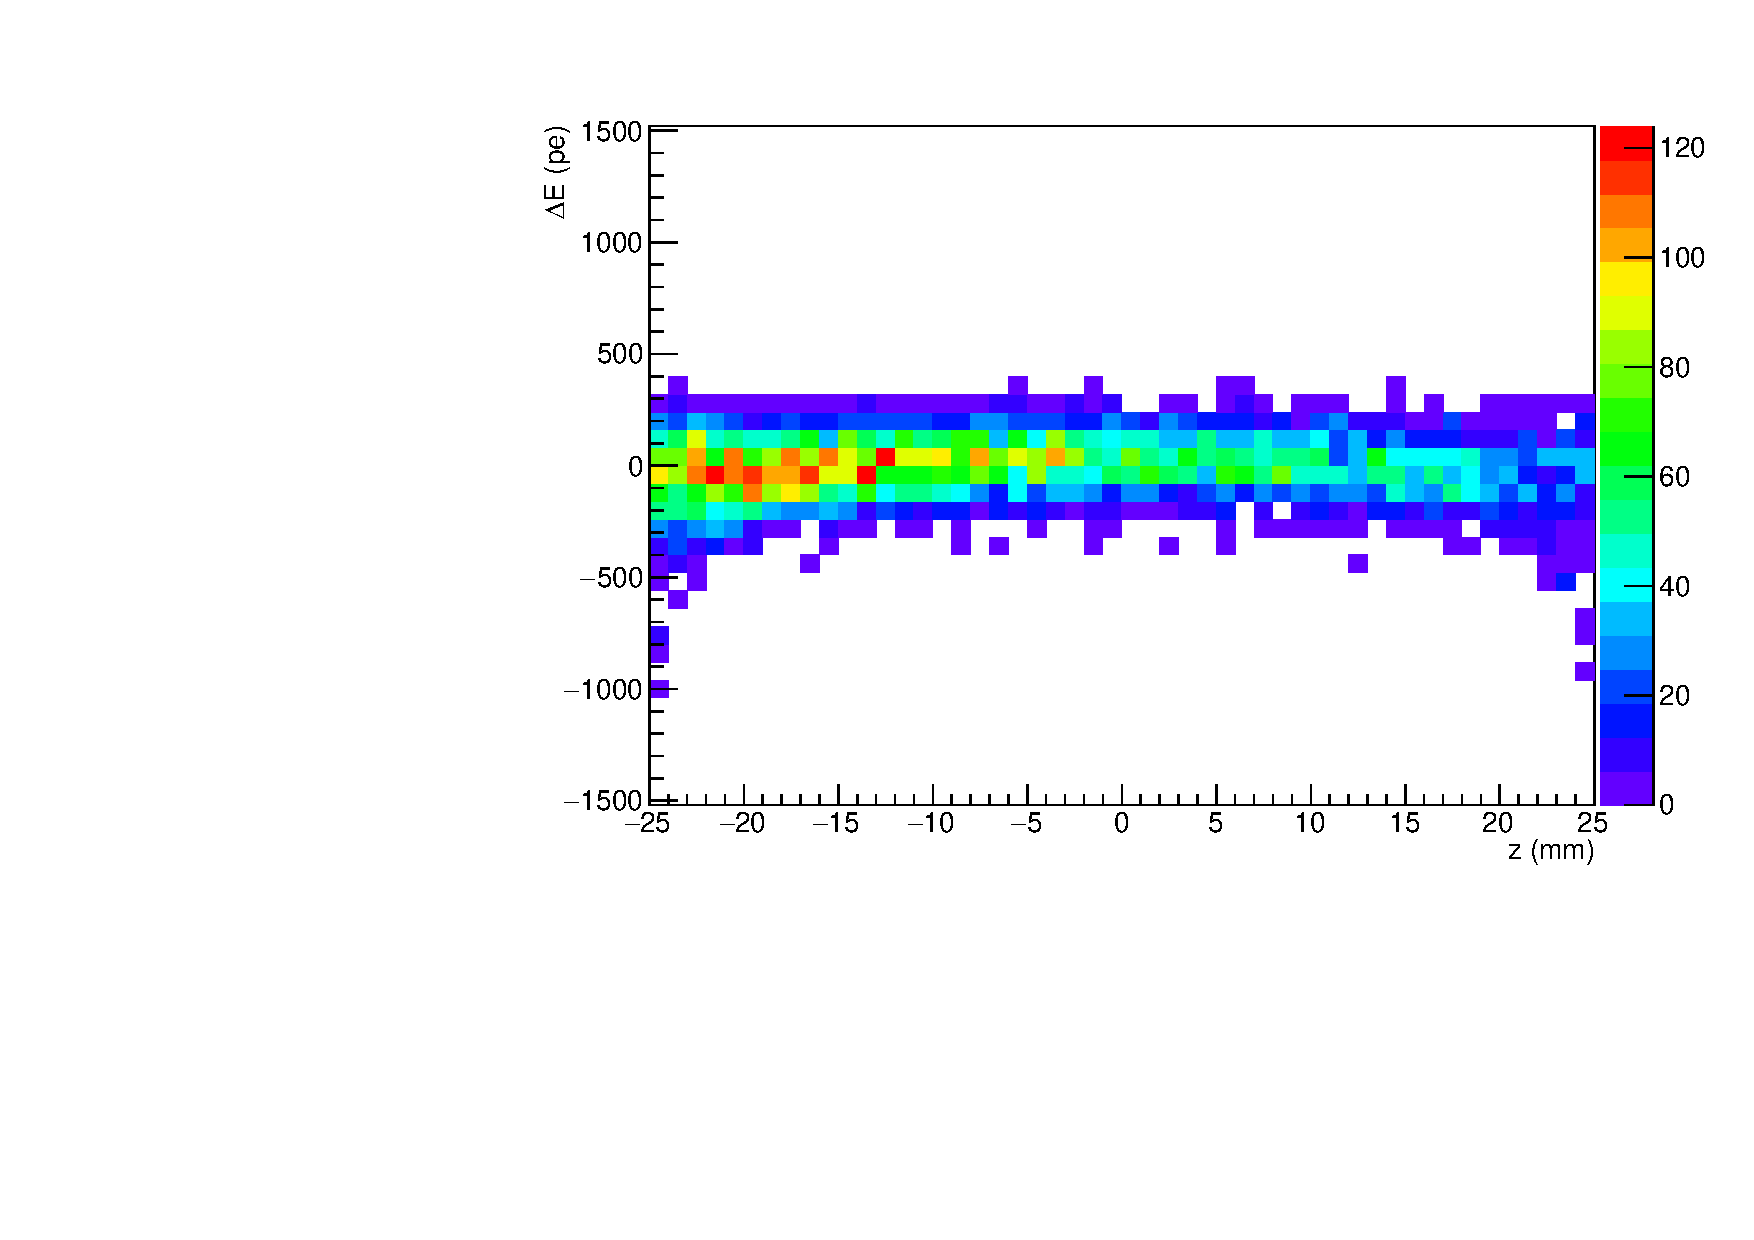
\includegraphics[width=.5\textwidth]{img/eposz_664.pdf}
				\label{fig.eposz664}				
			}\\
	\caption{\label{fig.energyDep6} Difference between the reconstructed energy and the average energy ($\Delta E$) as a function of one coordinate. (a) Energy dependence with the transverse coordinate ($x$) in LXSC6. (b) Energy dependence with the longitudinal coordinate ($z$) in LXSC6.}
\end{figure}			


\begin{figure}[!htb]
	\centering			
		\subfloat[LXSC4, $x$ coordinate]{
			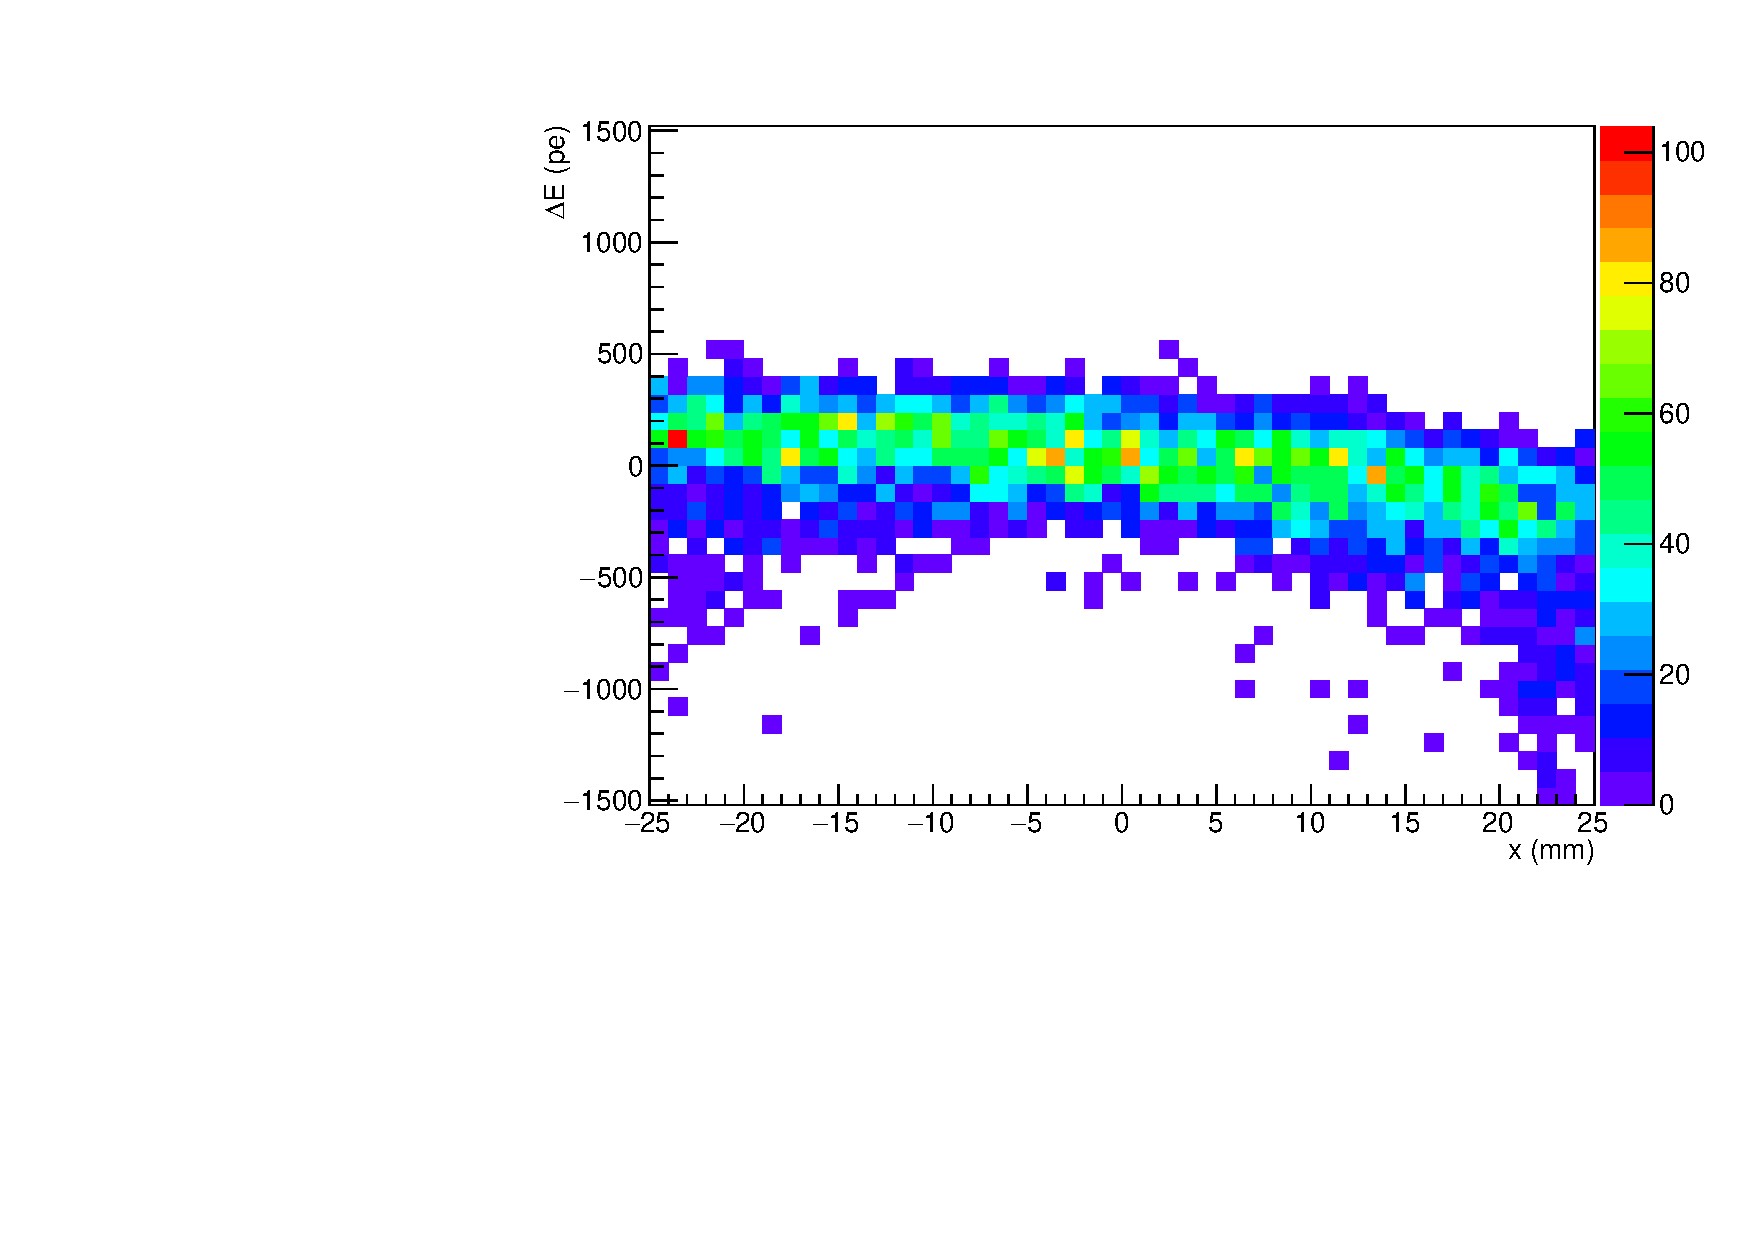
\includegraphics[width=.5\textwidth]{img/eposx_464.pdf}
			\label{fig.eposx464}
		}
		\subfloat[LXSC4, $z$ coordinate]{
			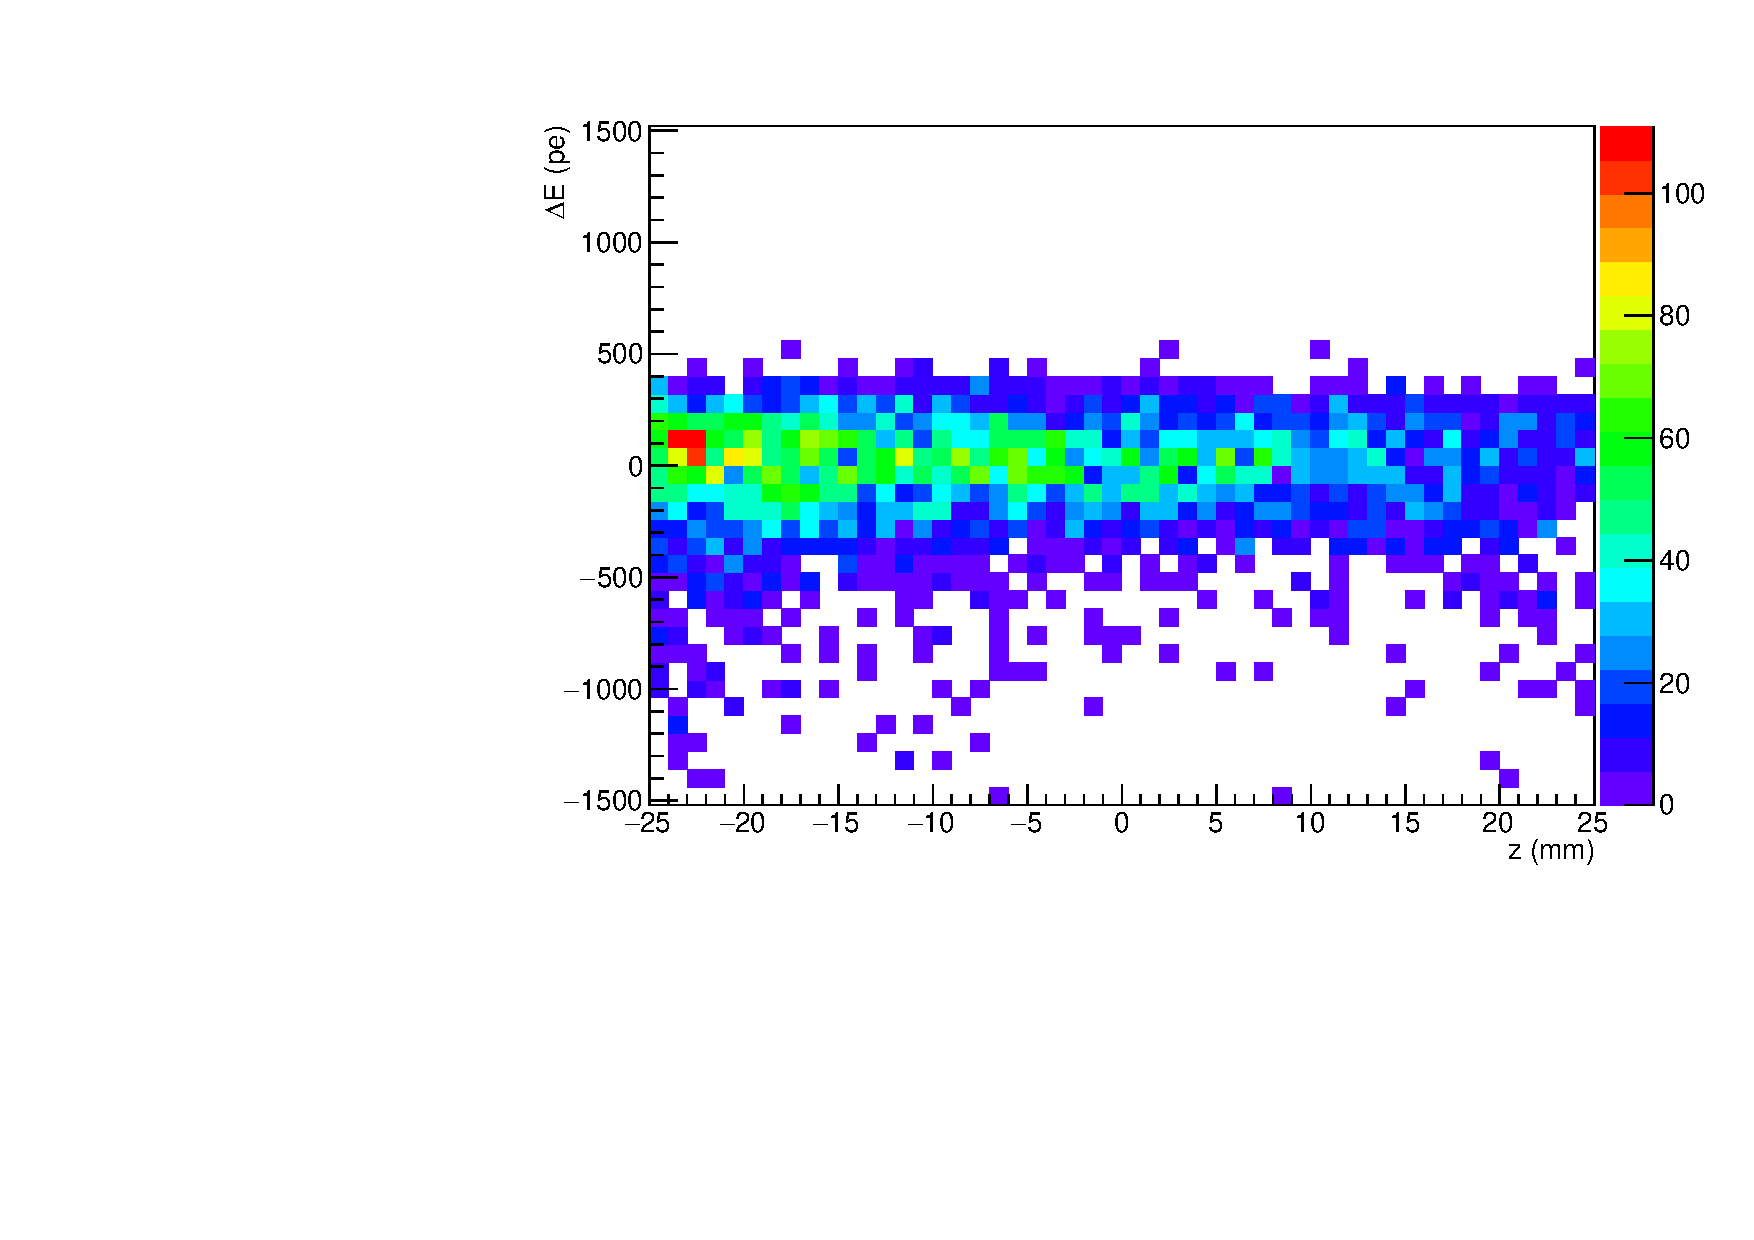
\includegraphics[width=.5\textwidth]{img/eposz_464.pdf}
			\label{fig.eposz464}				
		}\\
	\caption{\label{fig.energyDep4} Difference between the reconstructed energy and the average energy ($\Delta E$) as a function of one coordinate. (a) Energy dependence with the transverse coordinate ($x$) in LXSC4. (b) Energy dependence with the longitudinal coordinate ($z$) in LXSC4.}
\end{figure}		


\begin{figure}[!htb]
	\centering		
		\subfloat[LXSC2, $x$ coordinate]{
			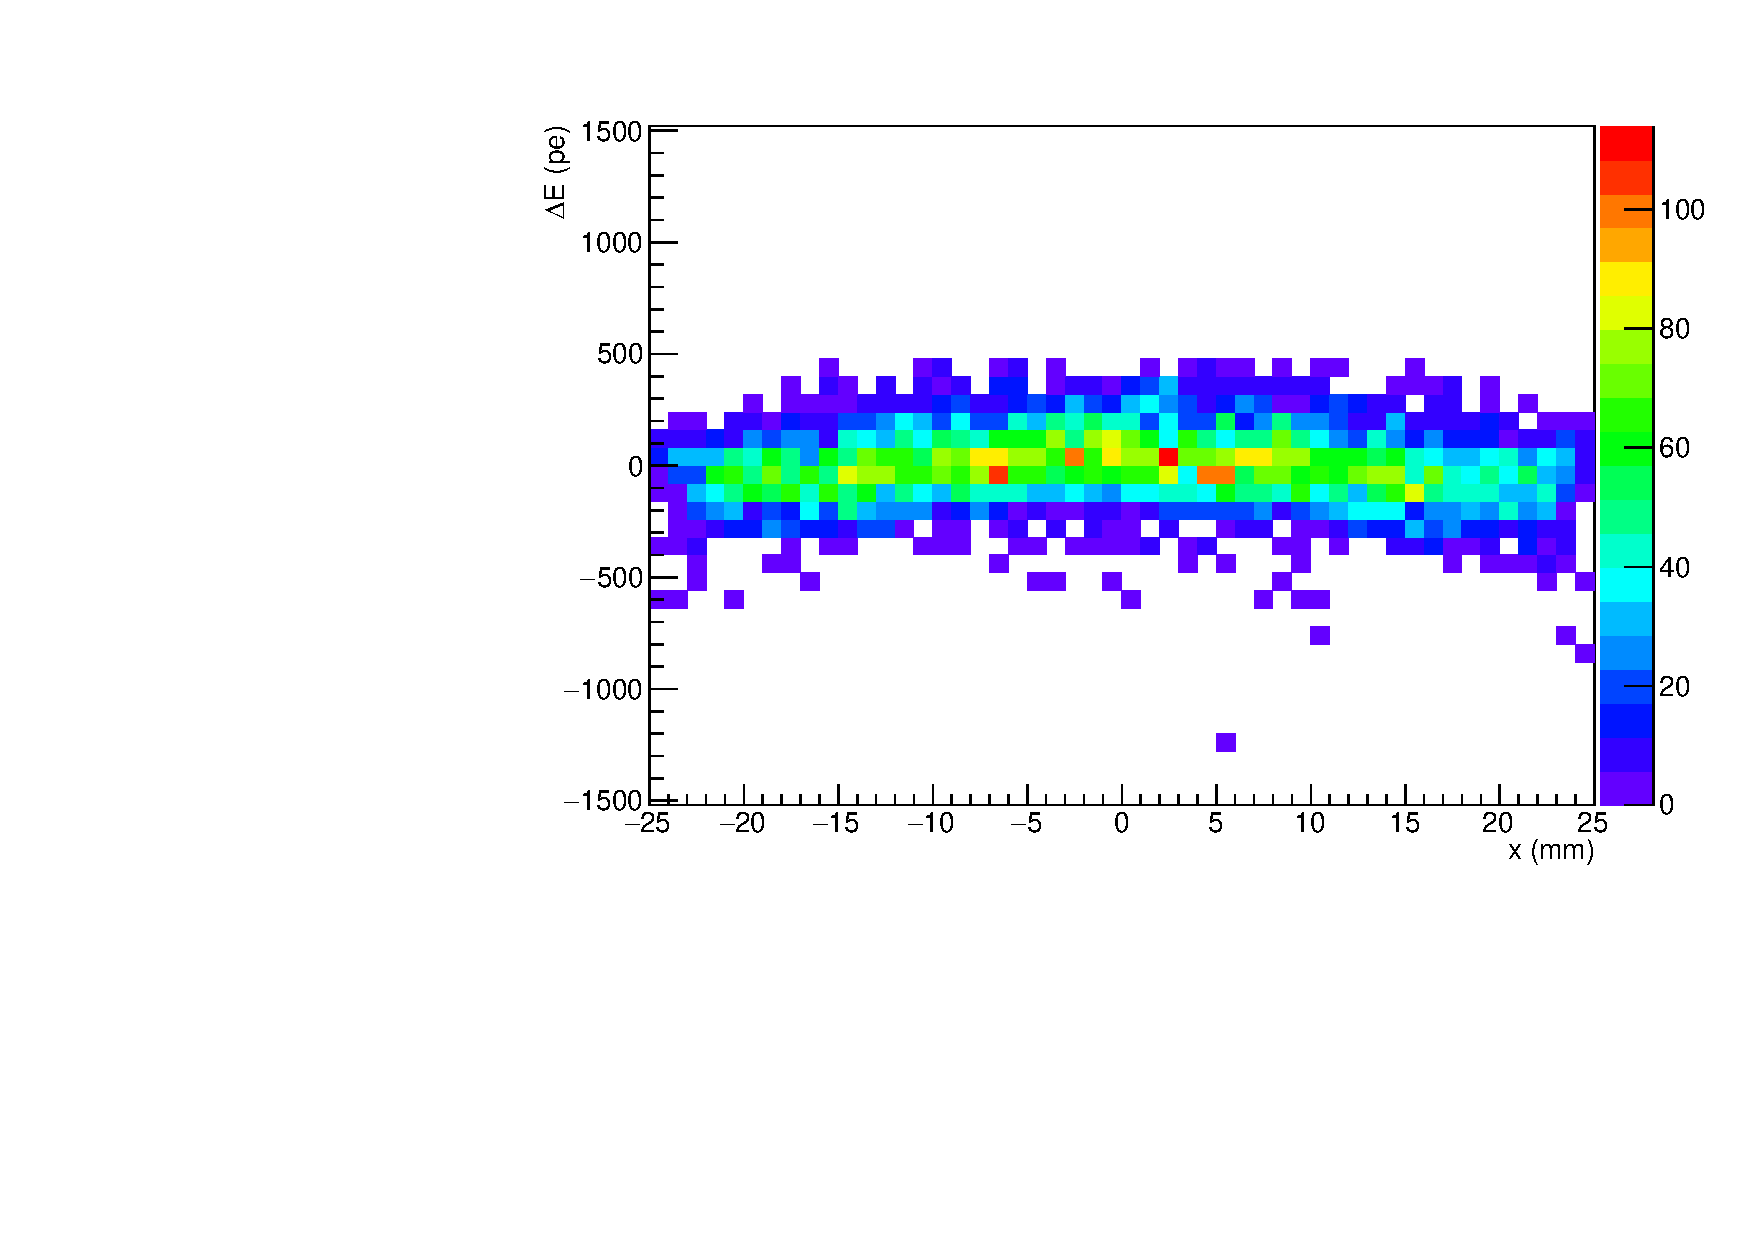
\includegraphics[width=.5\textwidth]{img/eposx_264.pdf}
			\label{fig.eposx264}
		}
		\subfloat[LXSC2, $z$ coordinate]{
			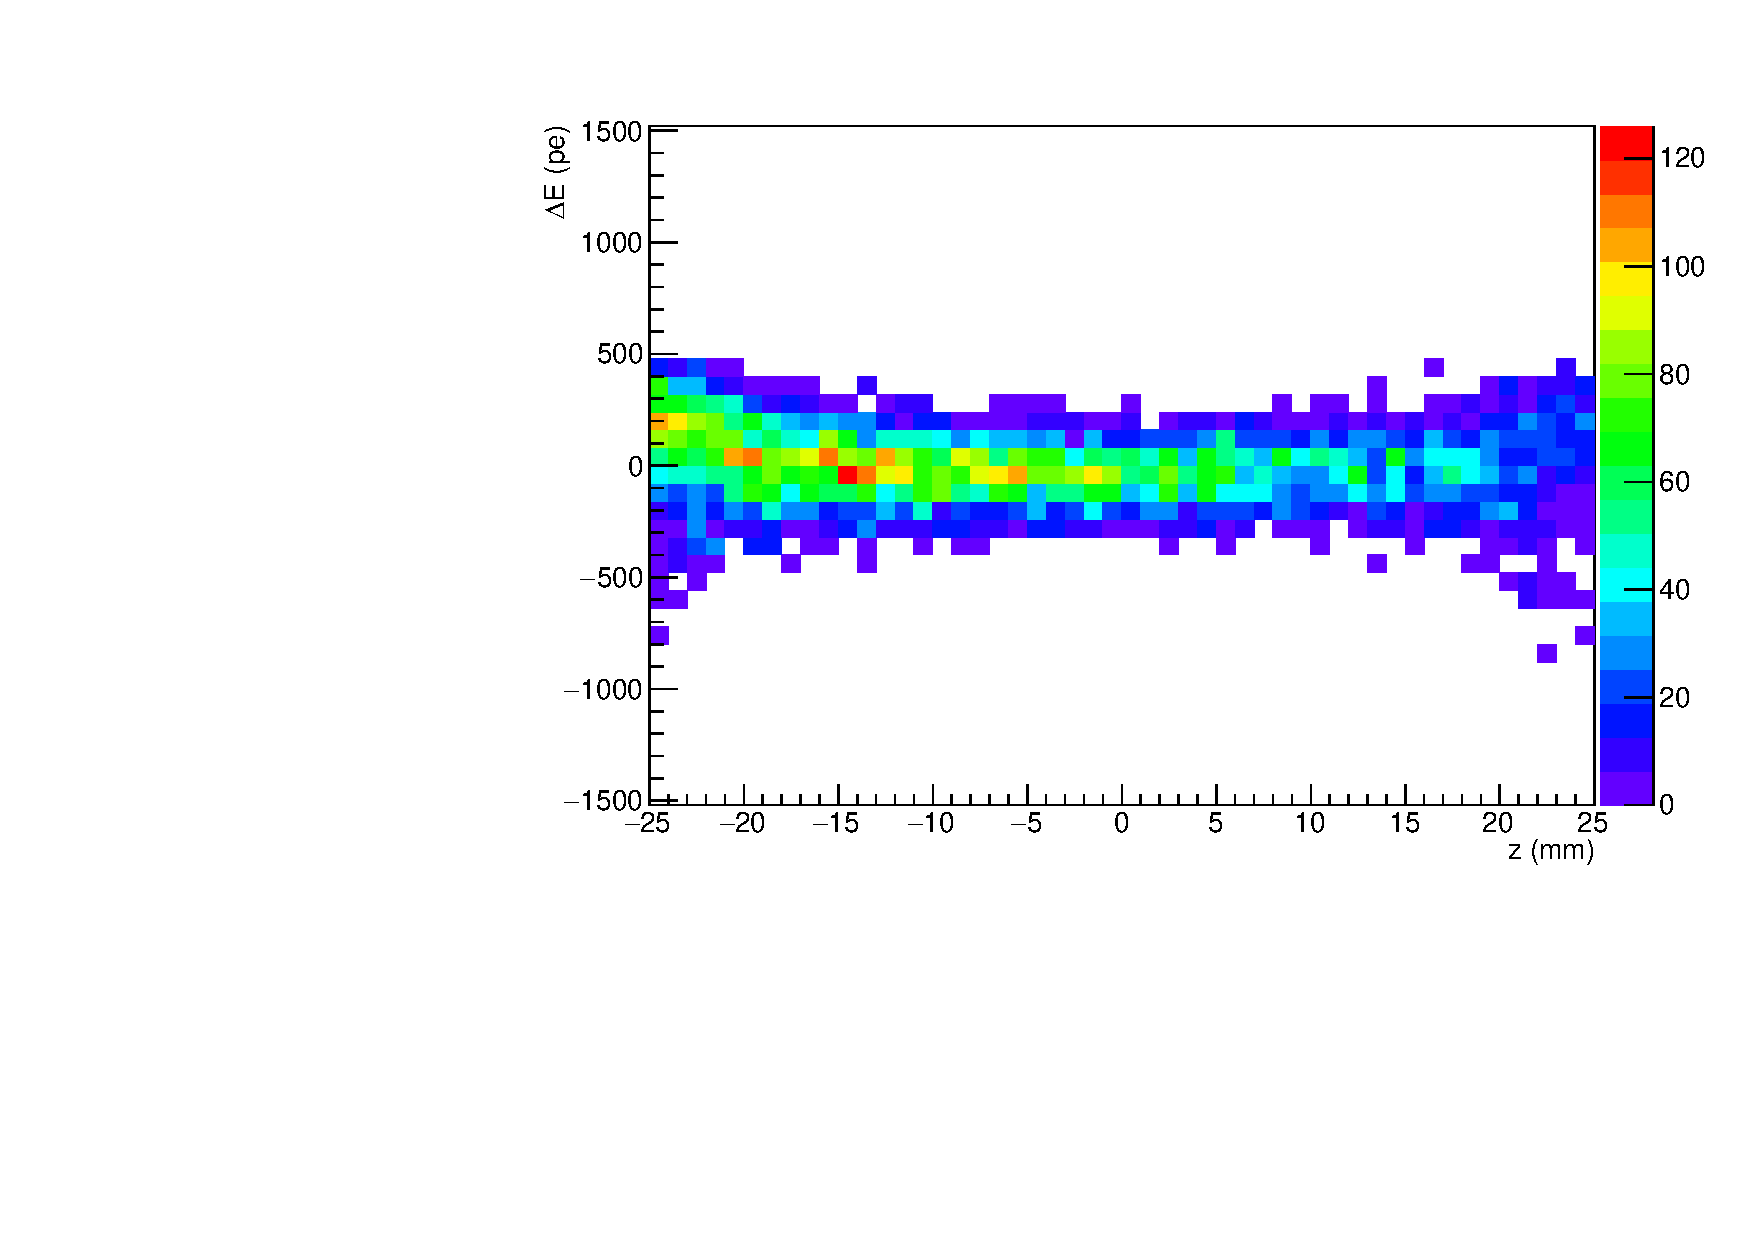
\includegraphics[width=.5\textwidth]{img/eposz_264.pdf}
			\label{fig.eposz264}
		}
	\caption{\label{fig.energyDep2} Difference between the reconstructed energy and the average energy ($\Delta E$) as a function of one coordinate. (a) Energy dependence with the transverse coordinate ($x$) in LXSC2. (b) Energy dependence with the longitudinal coordinate ($z$) in LXSC2.}
\end{figure}

The need for geometrical corrections is illustrated in Figures \ref{fig.energyDep6},\ref{fig.energyDep4} and \ref{fig.energyDep2}, which shows the difference between reconstructed energy and average energy as a function of one coordinate. The dependence of the energy with the longitudinal and transverse coordinate in the LXSC6 is very soft (Figures \ref{fig.eposx664} and \ref{fig.eposz664}), and can be neglected for all practical purposes. This is indeed expected, as the LXSC6 is totally symmetric and solid angle effects are minimized. If we decrease the amount of instrumentation, energy resolution worsens to around $\sim4\%$ for 49 SiPM and $\sim5\%$ for 36 SiPM. This is due to the geometrical corrections needed as we have covered less surface with sensors.

In the case of the LXSC4 (Figures \ref{fig.eposx464} and \ref{fig.eposz464}) the effect is larger due to the asymmetry of the detector giving resolutions of $\sim 4\%$. LXSC2 requires smaller corrections as is shown in Figures \ref{fig.eposx464} and \ref{fig.eposz464}, resolution in this case is $\sim 3.7\%$. Applying geometrical corrections one could improve the resolutions quoted.

%\begin{table}[h]
%\caption{\label{tab.energy1} Energy resolution (\% FWHM) for LXSC in function of the number of planes and the number of SiPM on each plane.}
%\begin{center}
% \begin{tabular}{c|ccc}
%  \toprule
%   Planes\textbackslash SiPM & \textbf{36 SiPM} & \textbf{49 SiPM} & \textbf{64 SiPM} \\
%   \hline
%  {\bf 2 Planes} & 3.7\% & 3.5\% & 3.7\%\\
%  {\bf 4 Planes} & 4.4\% & 4.1\%  & 3.9\%\\
%  {\bf 6 Planes} & 5.1\% & 4.1\% & 2.6\%\\
%  \toprule
% \end{tabular}
%\end{center}
%\end{table}

%\begin{table}[h]
%\begin{center}
%\caption{\label{tab.energy2} Energy resolution for LXSC2 varying longitudinal size.}
%  \begin{tabular}{c|c}
%   \toprule
%    Longitudinal size & \textbf{Resolution (FWHM)} \\
%    \hline
%   {\bf 2 cm} & 5.0\% \\
%   {\bf 3 cm} & 4.5\% \\
%   {\bf 4 cm} & 3.9\% \\
%   {\bf 5 cm} & 3.8\% \\
%   \toprule
%  \end{tabular}
% \end{center}
%\end{table}

Reducing the longitudinal size of the box has also an effect on resolution. We have studied this effect on LXSC2. Resolution is 3.7\% for 5 cm and 5\% for 2 cm. The resolution worsens due to energy losses, but is still acceptable. 

Finally, if we assume the lowest $W_{ph}$~measured for electrons
(24,000 photons rather than 37,000 photons for a 511 keV gamma)
 the yield would be reduced by 65\% and the resolution of the LXSC2 would be spoiled by a factor $1./\sqrt{0.65} = 1.2$. One would then have a resolution of around 4.5\% FWHM, still much better than that of modern SSDs such as LSO/LYSO.

Notice that the small geometrical corrections found in the LXSC are a crucial difference with the Waseda cell, where the geometrical corrections, due to the large size of the PMTs where very large (see Figure \ref{fig.wasedaGeo}) and made, ultimately, the cell impractical as a detection device, since only the central part of the detector ($5 \times 5 \times 5$~mm$^3$) was useful. The second crucial difference that the LXSC registers much more light than the Waseda cell. This is due to the fact that all the faces are reflecting (the Waseda cell left one face open, resulting in large losses and fluctuations) and to the use of SiPMs, which have very large PDE ($\sim$ 50\% to be compared with the 5-20\% of the Waseda PMTs) right in the region (420 nm) where the light is shifted from TPB. 

\begin{figure}[!htb]
	\centering
	\subfloat[LXSC6-64]{
		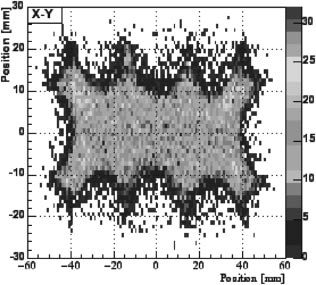
\includegraphics[width=.33\textwidth]{img/xy_waseda.png}
	}
	\subfloat[LXSC2-36]{
		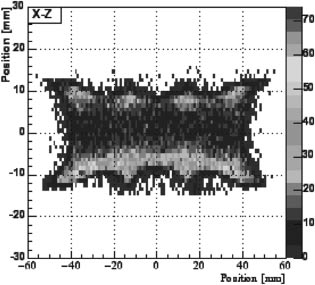
\includegraphics[width=.33\textwidth]{img/xz_waseda.png}
	}
	\subfloat[LXSC2-36]{
		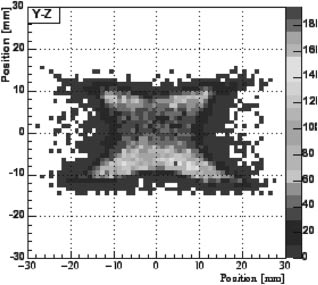
\includegraphics[width=.33\textwidth]{img/yz_waseda.png}
	}
	\caption{\label{fig.wasedaGeo} Position distributions of interaction points for annihilation gamma rays in the Waseda cell \cite{nishikido05}. Very large geometrical corrections are needed. (a) XY distribution, (b) XZ distribution and (c) YZ YZ distribution.}
\end{figure}

%\newpage\null\thispagestyle{empty}\newpage
%\thispagestyle{newstyle}
\subsection{Spatial resolution of the LXSC}
\label{sec.spatial}

\subsubsection*{Barycenter algorithm}
The simplest way to determine the point of interaction of an incoming photon, $(x,y,z)$~ is to use a barycenter algorithm. 
\[
\xi_r = \frac{\sum \xi_i N_i}{N}
\]
where $\xi_r$~stands for each one of the three coordinates ($x_r, y_r, z_r$), $N_i$~is the number of photoelectrons registered in each SiPM and $N=\sum N_i$. In the LXSC6 and LXSC4 configurations one can compute redundant measurements of $\xi_r$~for each coordinate. In the LXSC2 one can obtain ($x_r,y_r$) redundantly from the information found in the entry and exit faces and $z_r$~from the ratio of energy measured in the entry and the exit faces. To get a bound for the spatial resolution in our simulations we have chosen the best value for each coordinate. This could also be approximated using the charge recorded by each plane as a estimator of distance, thus we can select the best plane for each case as the one with more charge recorded.

Figures \ref{fig.photoelectricA} and \ref{fig.photoelectricB} show the signal recorded by entry and exit planes respectively for one event a few millimiters away from entry plane. The interaction vertex is clearly visible in the entry plane but not in the other. If the interaction takes place near the center of the box, then the vertex is blurred in both planes (Figures \ref{fig.photoelectricC} and \ref{fig.photoelectricD}). Finally, the effect is the opposite for an event taking place near the exit plane (Figures \ref{fig.photoelectricE} and \ref{fig.photoelectricF}). 

The effect of the box thickness is illustrated quantitatively in Figure \ref{fig.sipmm}, which shows the number of photoelectrons in the SiPM registering the maximum signal (max signal sensor or MSS) as a function of the distance to the entry face (\ref{fig.simpmmc_p0}) and the number of photoelectrons in the SiPMs registering the maximum signal as a function of the distance to the exit face (\ref{fig.simpmmc_p2}). The signal of the MSS stays above 100 pes for the first (and the last) 2 cm of the cell, therefore we can use the entry face signal in one case, and the exit face signal in the other. In the central volume of about 1 cm, the position can be determined by the combination of the signal found in both faces.

Figure \ref{fig.zratio} shows the ratio of the signal in the entry and the exit face (the signal in a face is defined as the sum of the signals of all its SiPMs) as a function of the longitudinal coordinate. This ratio measures the longitudinal coordinate.  

\begin{figure}[H]
	\centering
	\subfloat[][Charge recorded in entry plane ($z=-25$) \\ for an event at $z=-18.81$.]{
		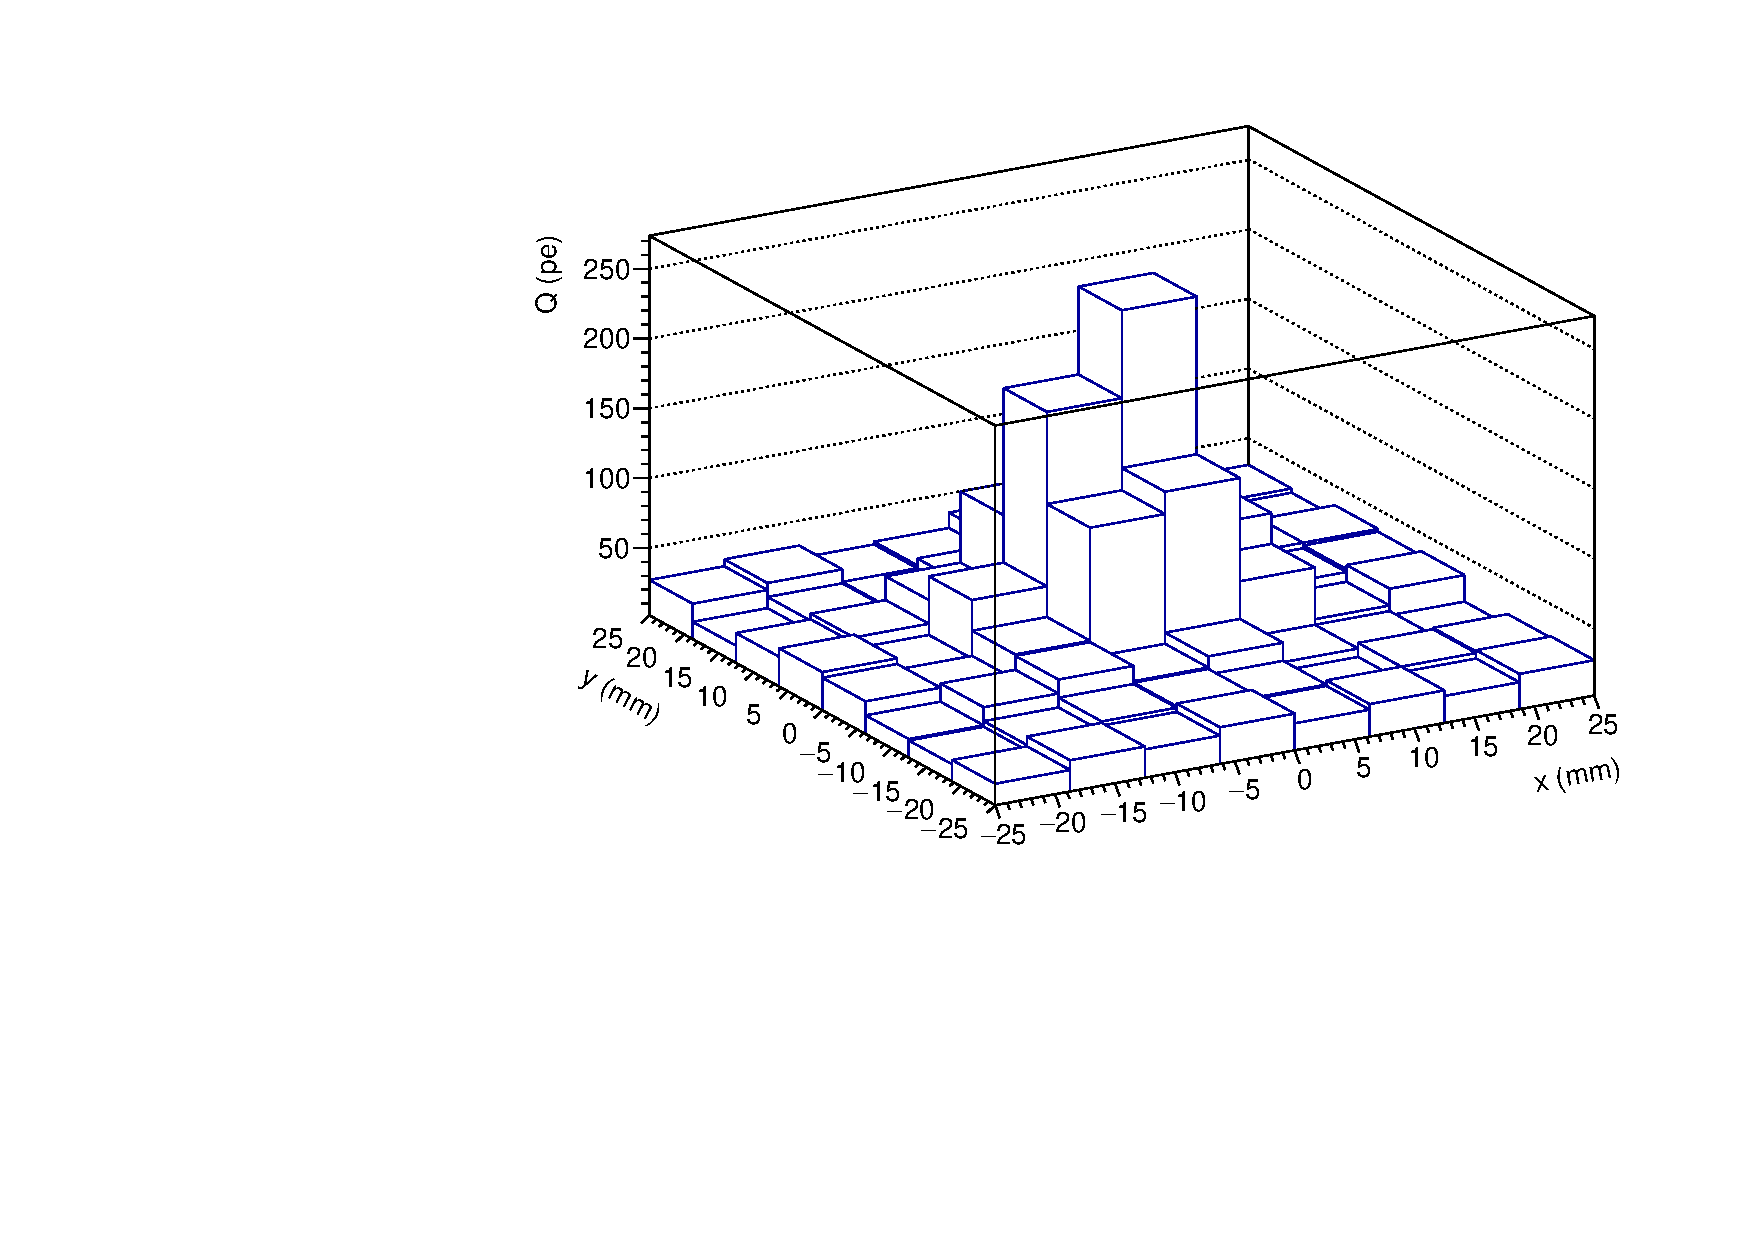
\includegraphics[width=.5\textwidth]{img/photoelectric_in_znear.pdf}
		\label{fig.photoelectricA}
	}
	\subfloat[][Charge recorded in exit plane ($z=25$) \\ for an event at $z=-18.81$.]{
		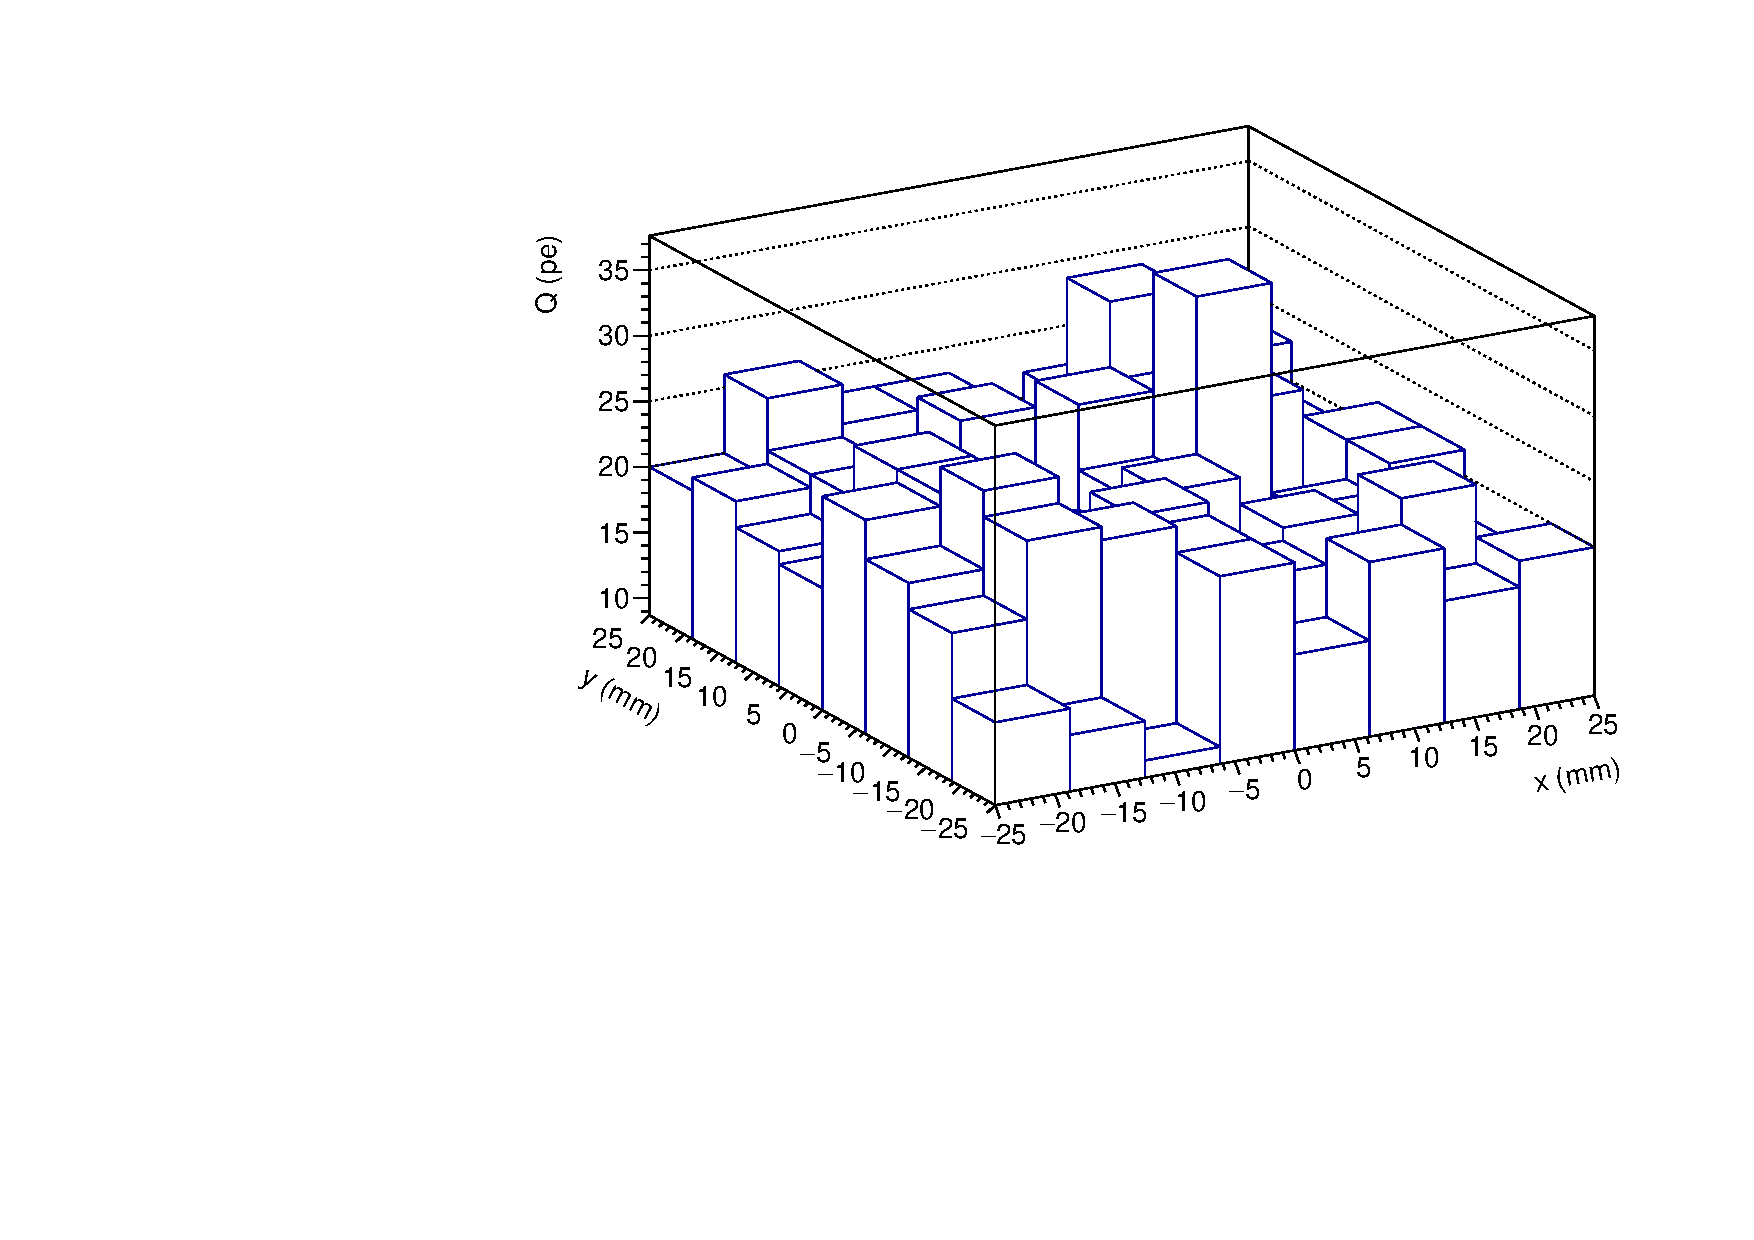
\includegraphics[width=.5\textwidth]{img/photoelectric_out_znear.pdf}
		\label{fig.photoelectricB}
	}\\
	\vspace{-0.5cm}
	\subfloat[][Charge recorded in entry plane ($z=-25$) \\ for an event at $z=1.96$.]{
		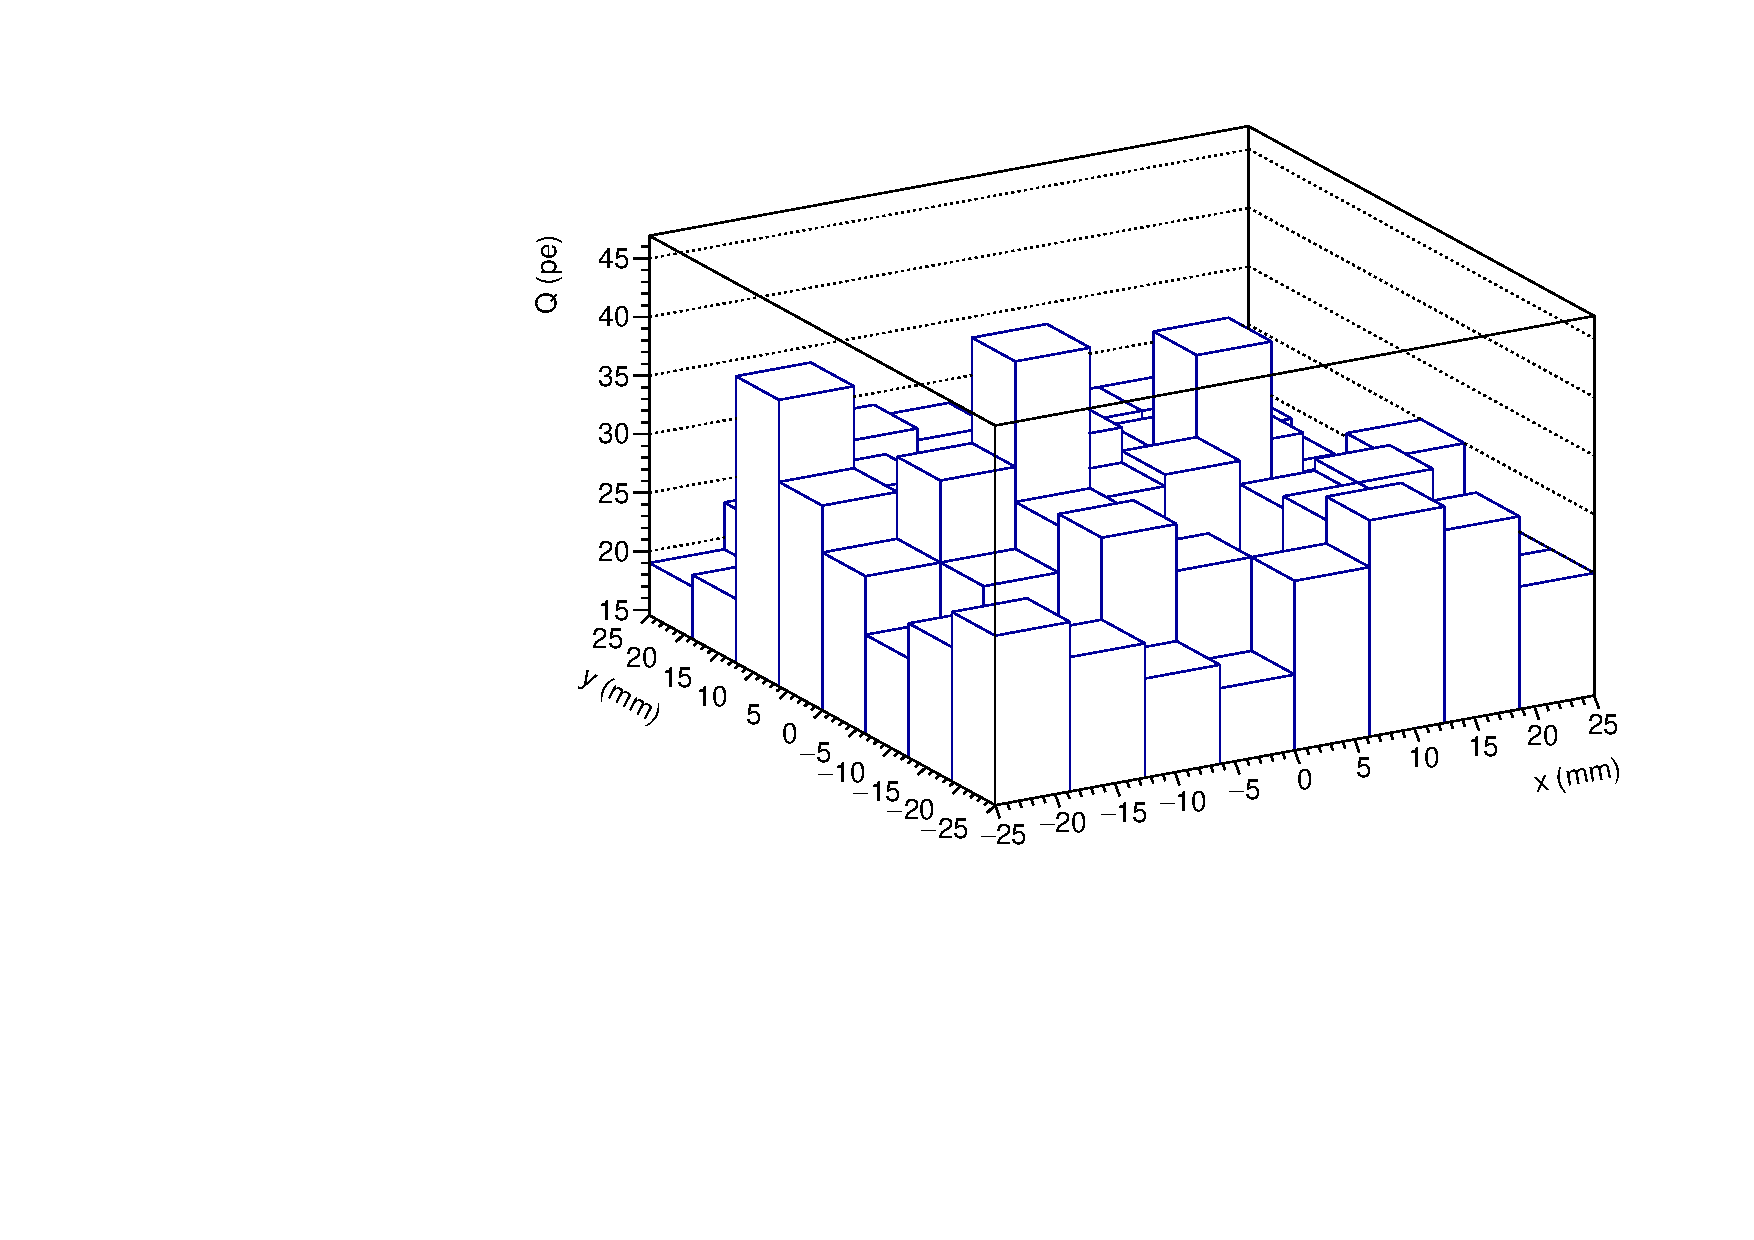
\includegraphics[width=.5\textwidth]{img/photoelectric_in_zmiddle.pdf}
		\label{fig.photoelectricC}
	}
	\subfloat[][Charge recorded in exit plane ($z=25$) \\ for an event at $z=1.96$.]{
		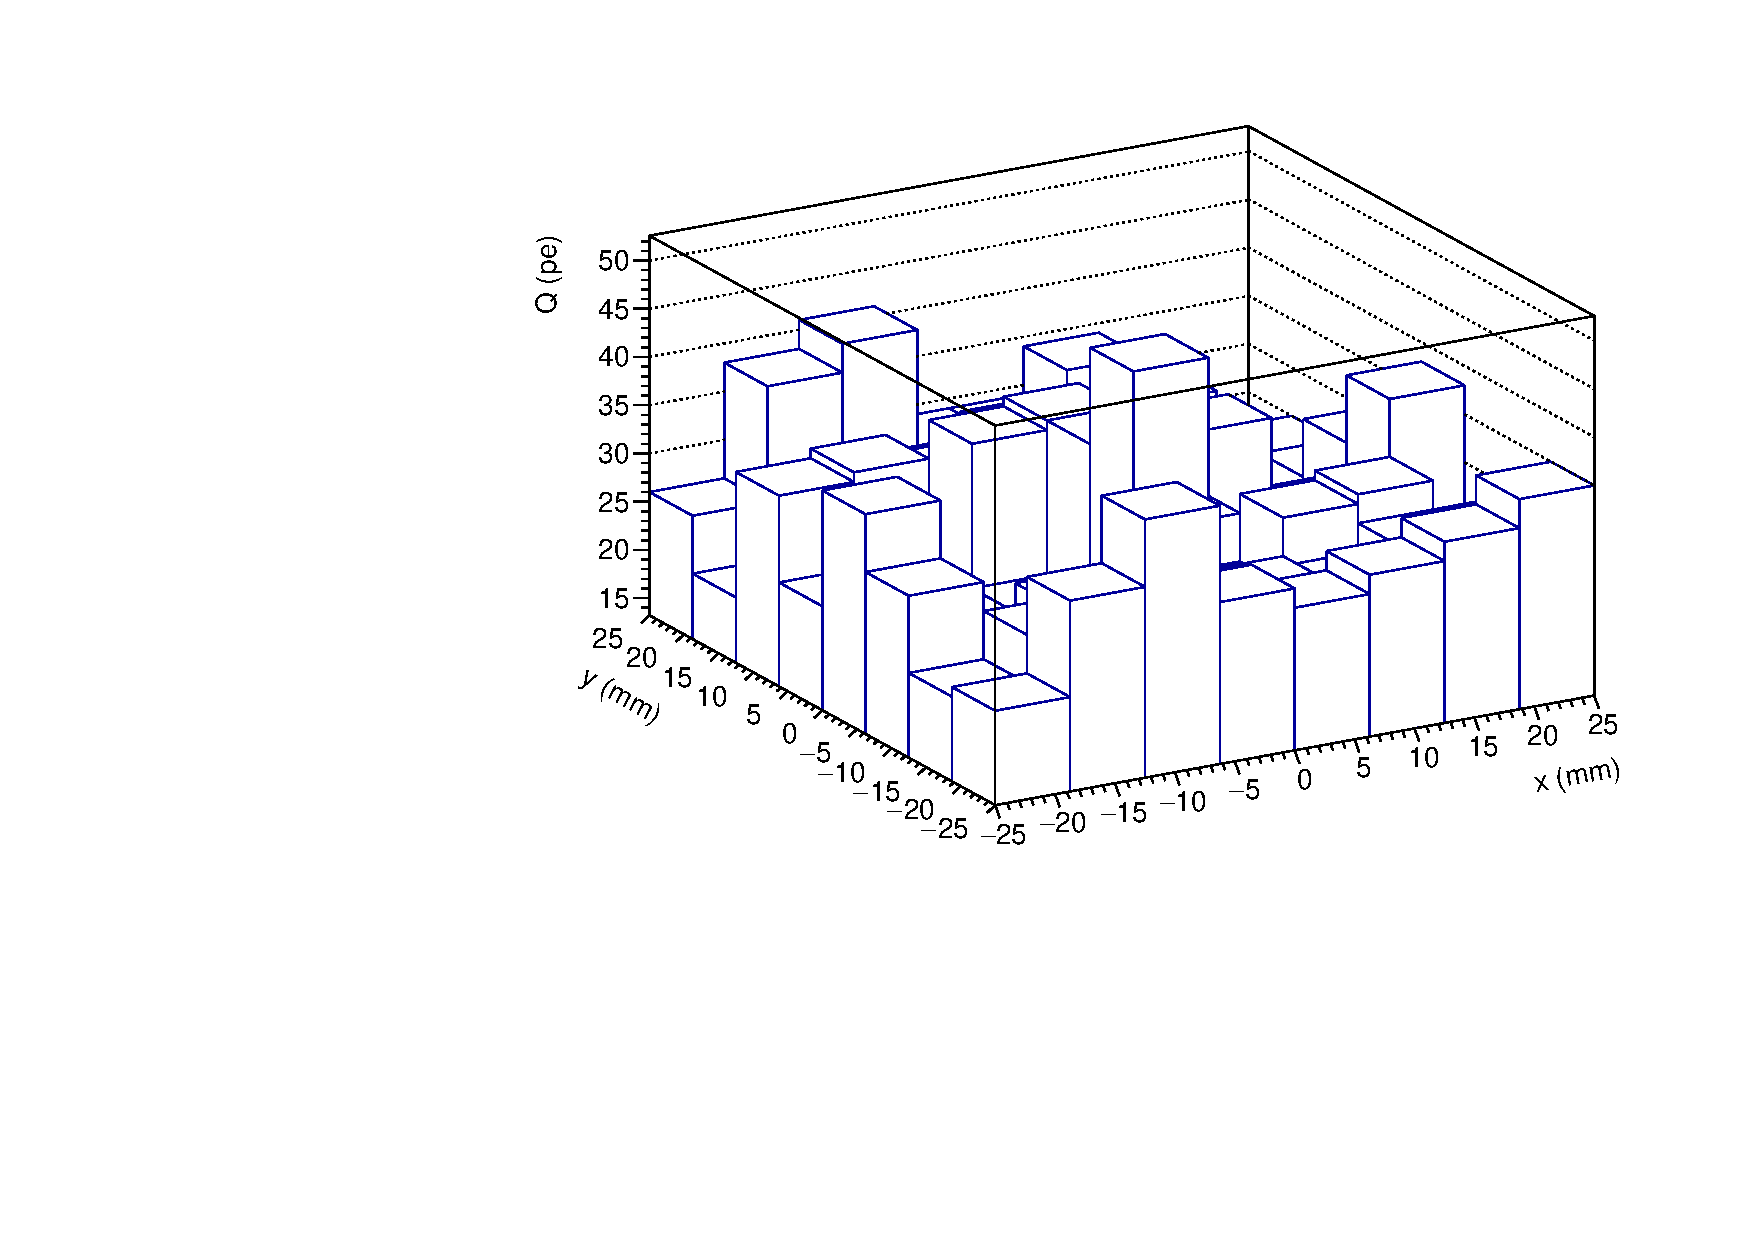
\includegraphics[width=.5\textwidth]{img/photoelectric_out_zmiddle.pdf}
		\label{fig.photoelectricD}
	}\\
	\vspace{-0.5cm}
	\subfloat[][Charge recorded in entry plane ($z=-25$) \\ for an event at $z=16.89$.]{
		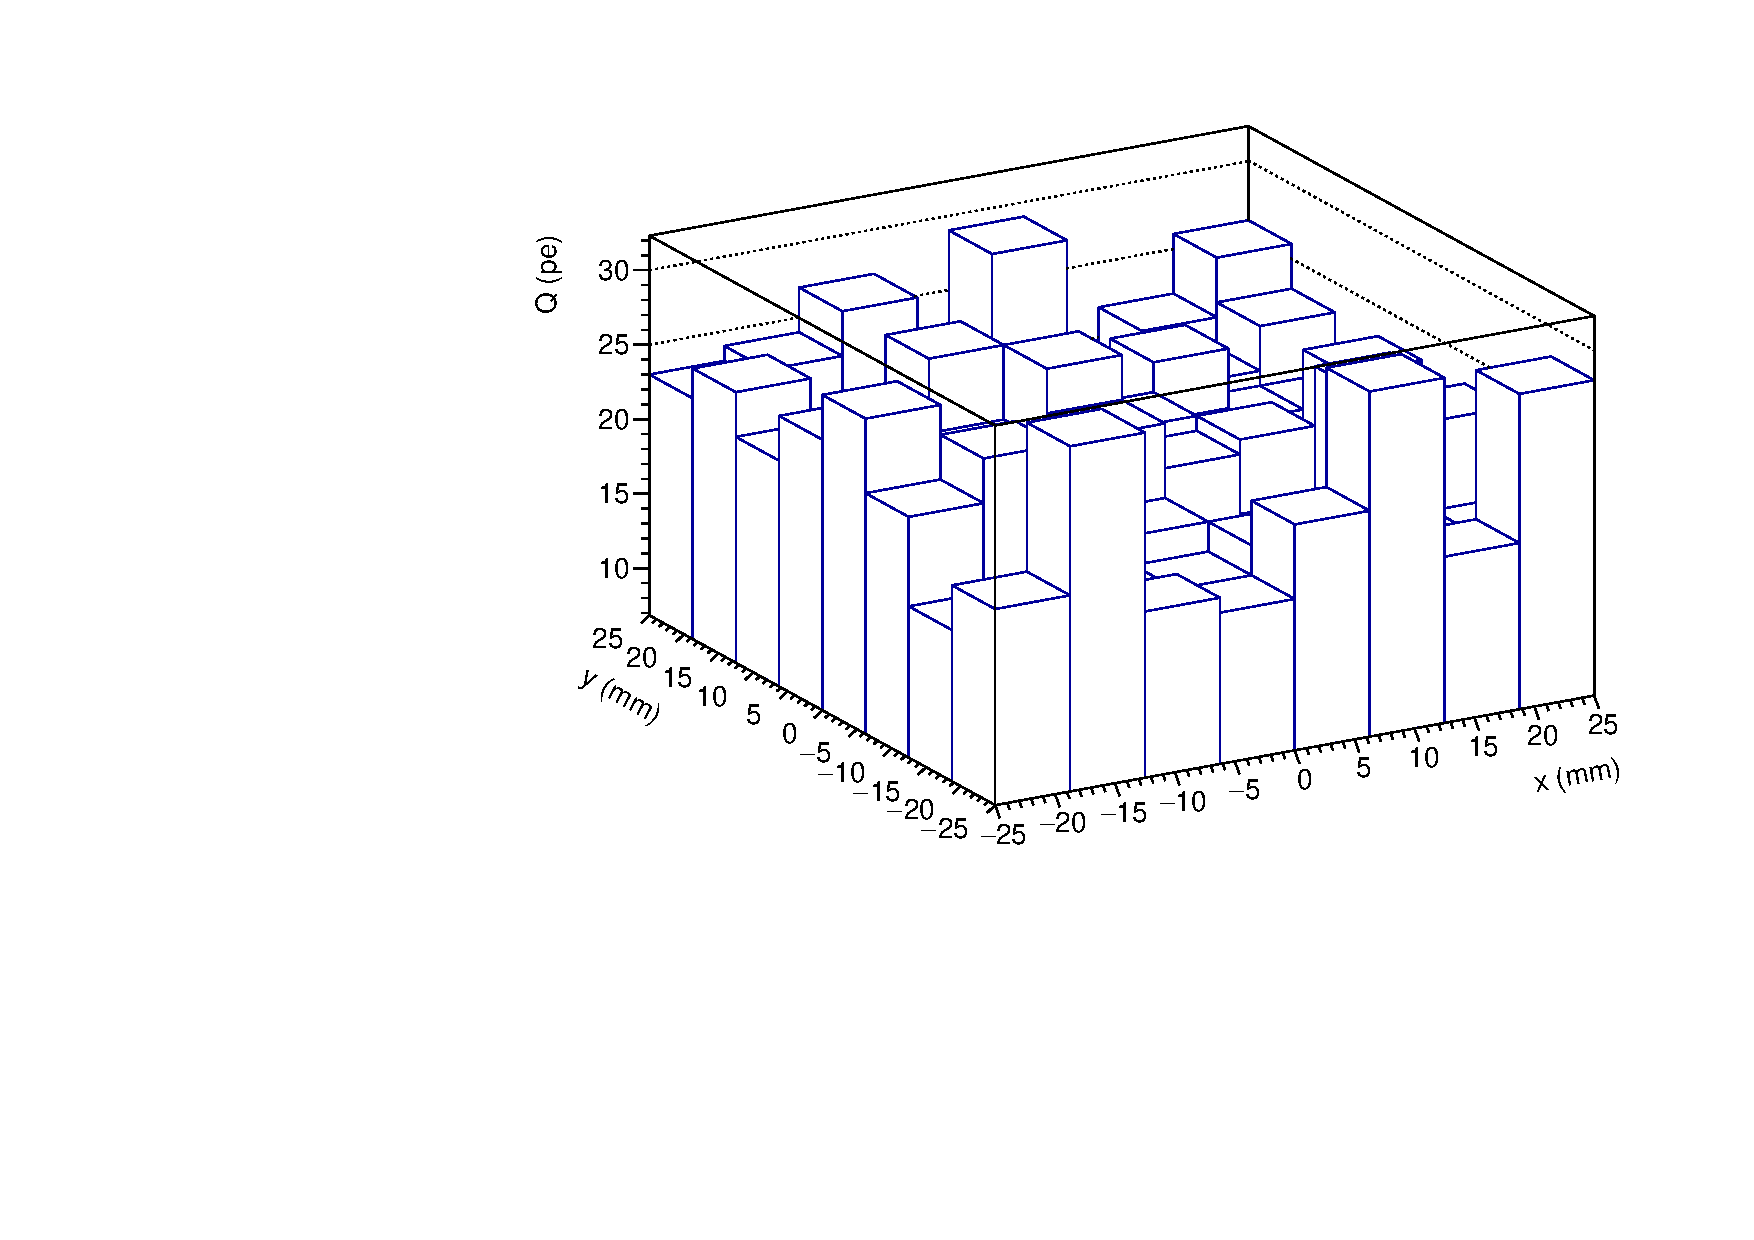
\includegraphics[width=.5\textwidth]{img/photoelectric_in_zfar.pdf}
		\label{fig.photoelectricE}
	}
	\subfloat[][Charge recorded in exit plane ($z=25$) \\ for an event at $z=16.89$.]{
		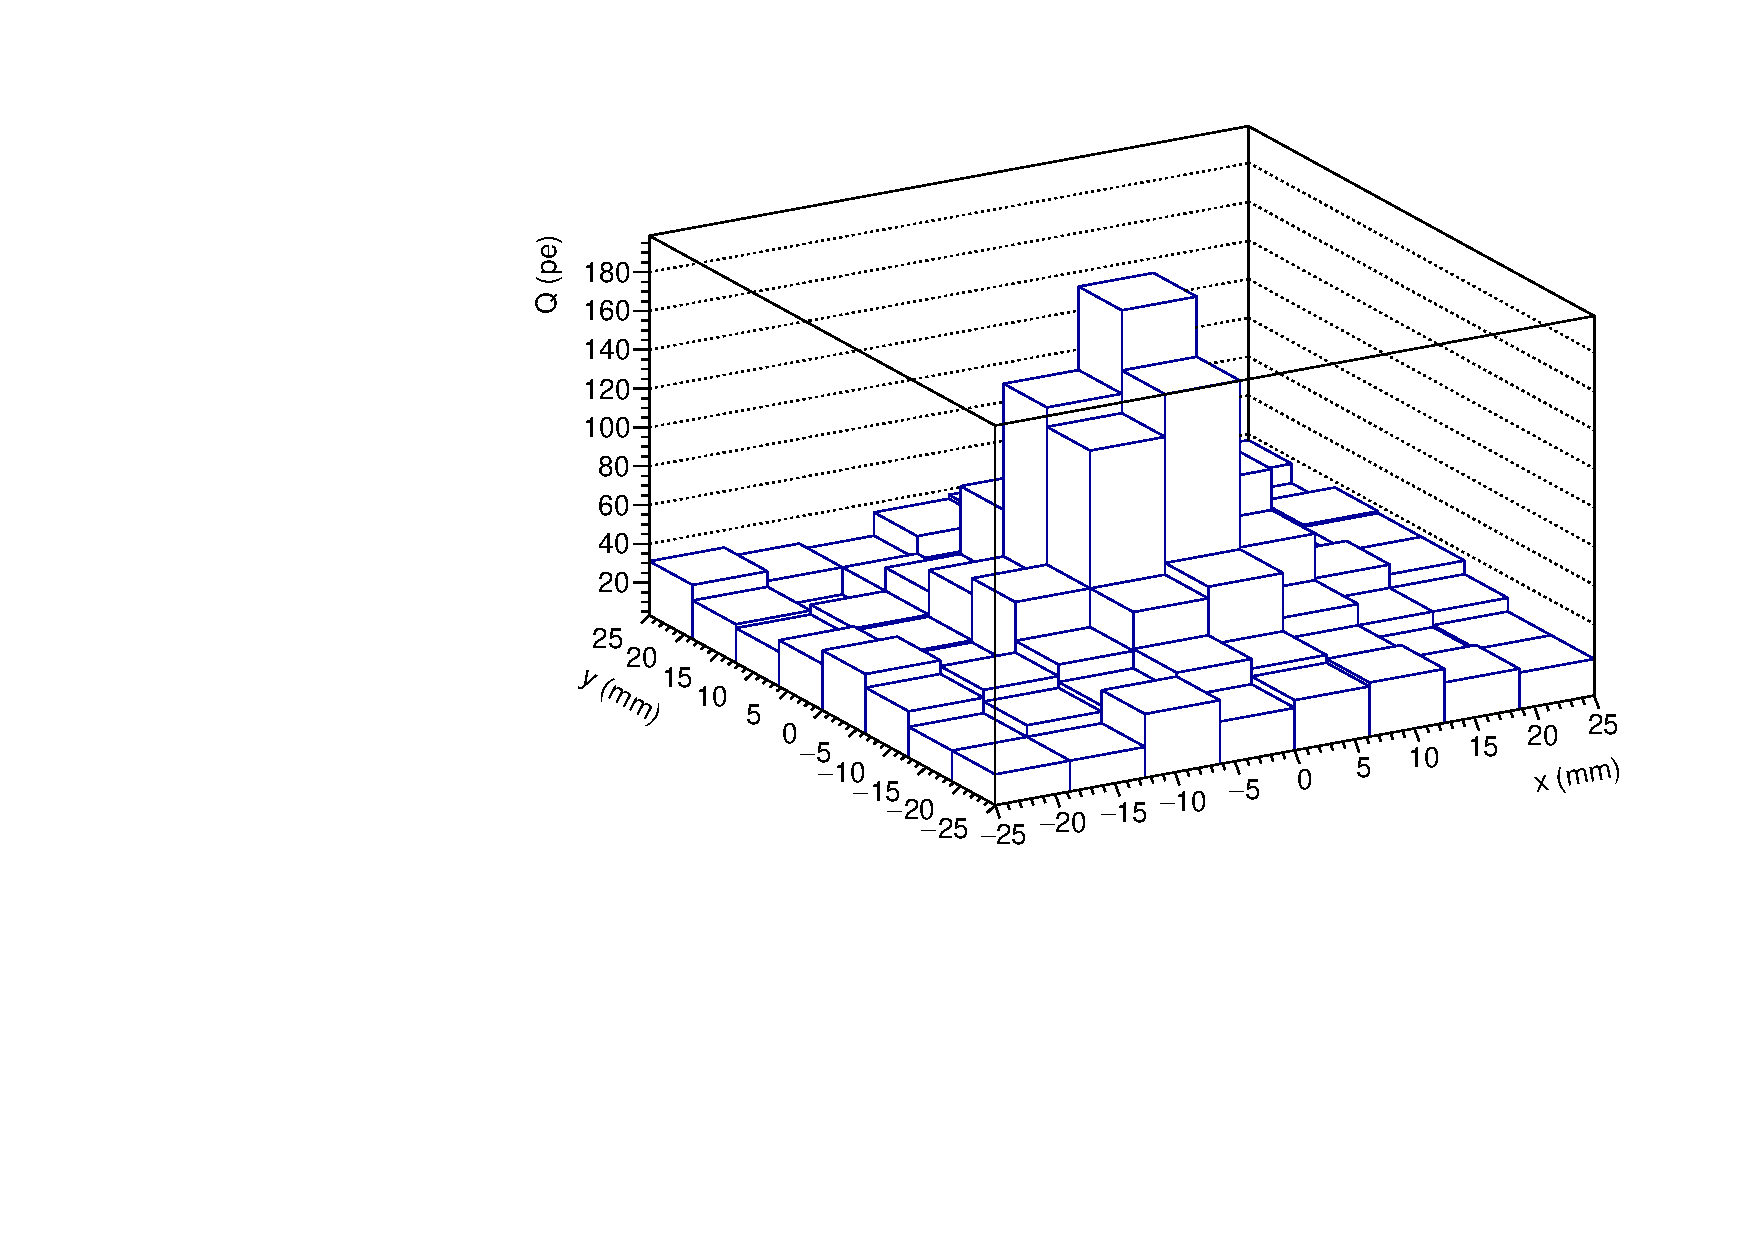
\includegraphics[width=.5\textwidth]{img/photoelectric_out_zfar.pdf}
		\label{fig.photoelectricF}
	}\\
	\caption{ \label{fig.photoelectric} Charge deposited on entry/exit plane for photoelectric events at several positions. Each row shows the same event as it is seen on each plane (entry on the left and exit on the right). First row shows an event at (1.26, 2.62,-18.81), second row at (0.63,-1.36,1.96) and the third at (0.88,0.46,16.89).}
\end{figure}

\begin{figure}[!htb]
	\centering
	\subfloat[Entry plane]{
		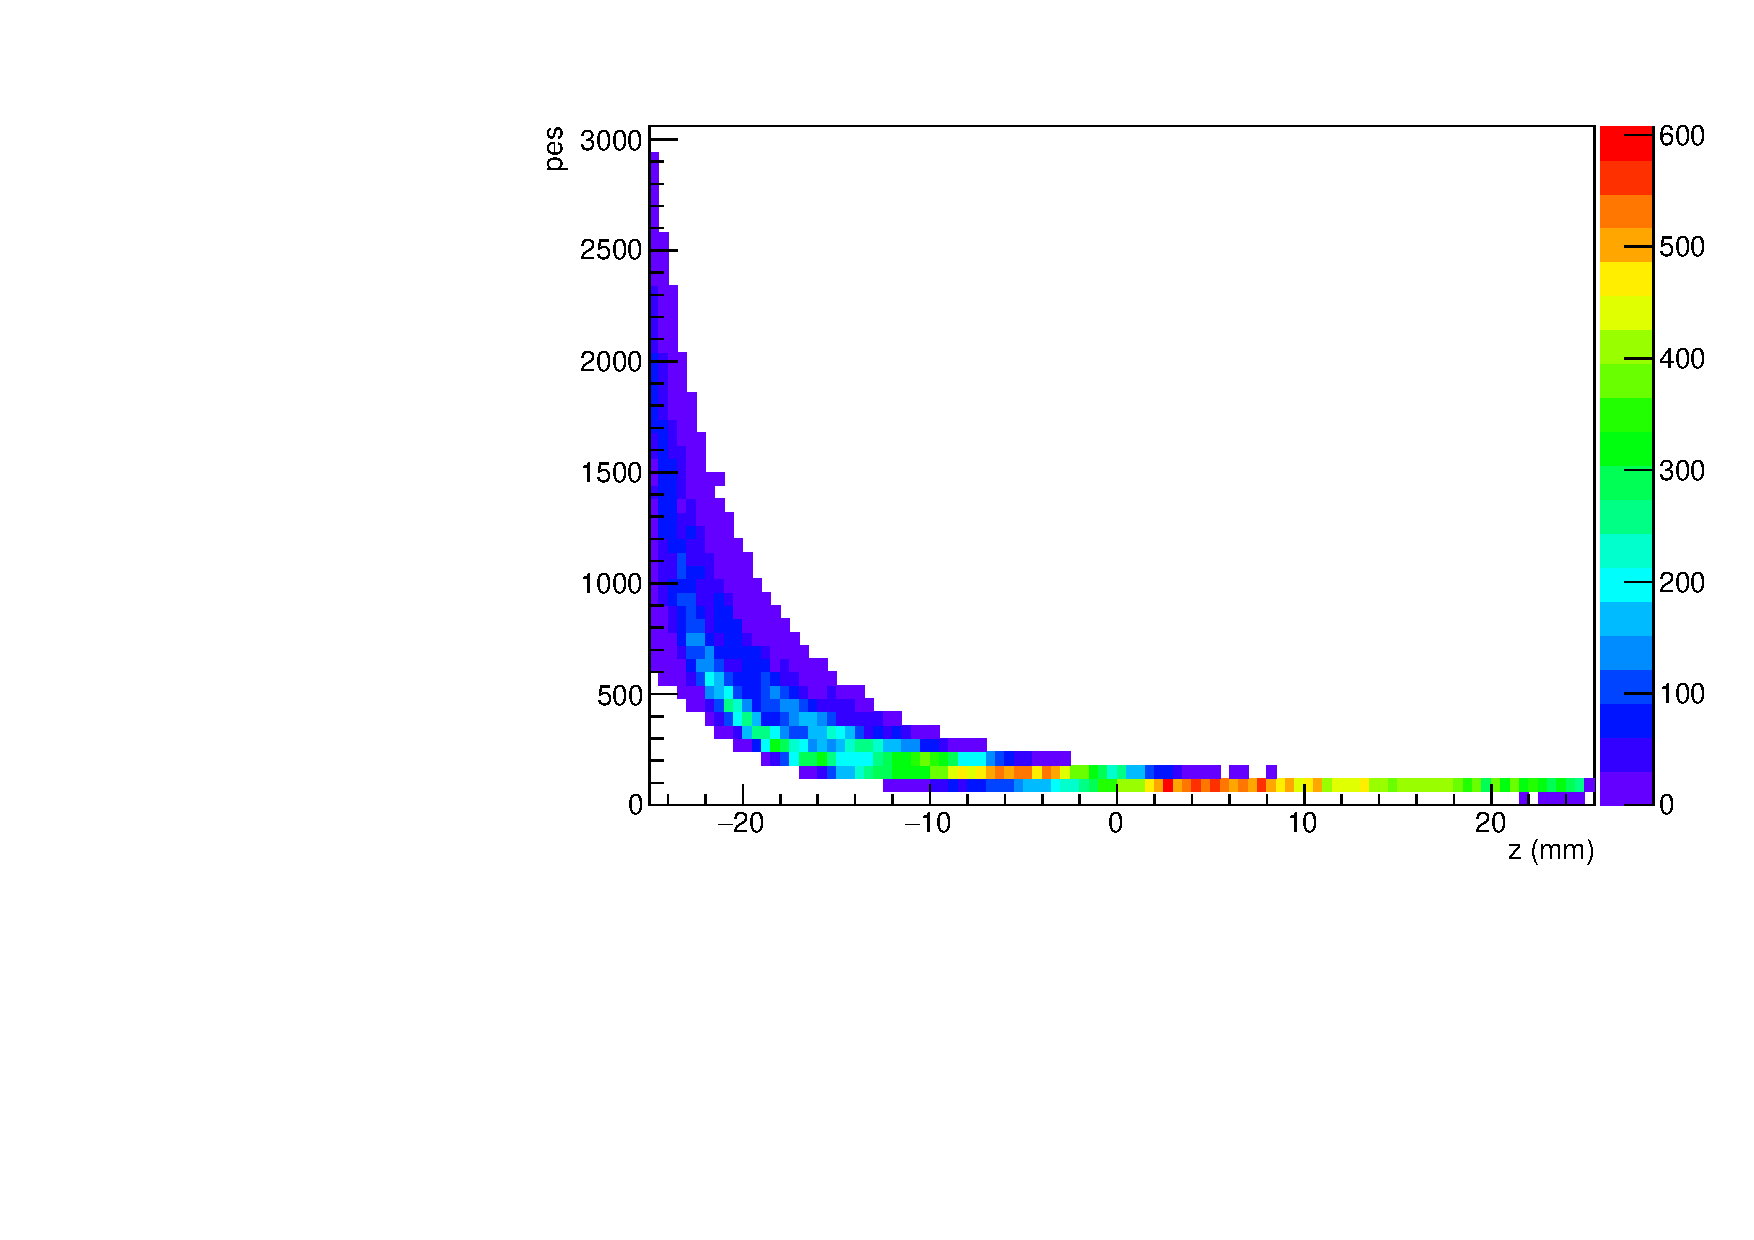
\includegraphics[width=.5\textwidth]{img/sipmmc_p0_2_z5.pdf}
		\label{fig.simpmmc_p0}
	}
	\subfloat[Exit plane]{
		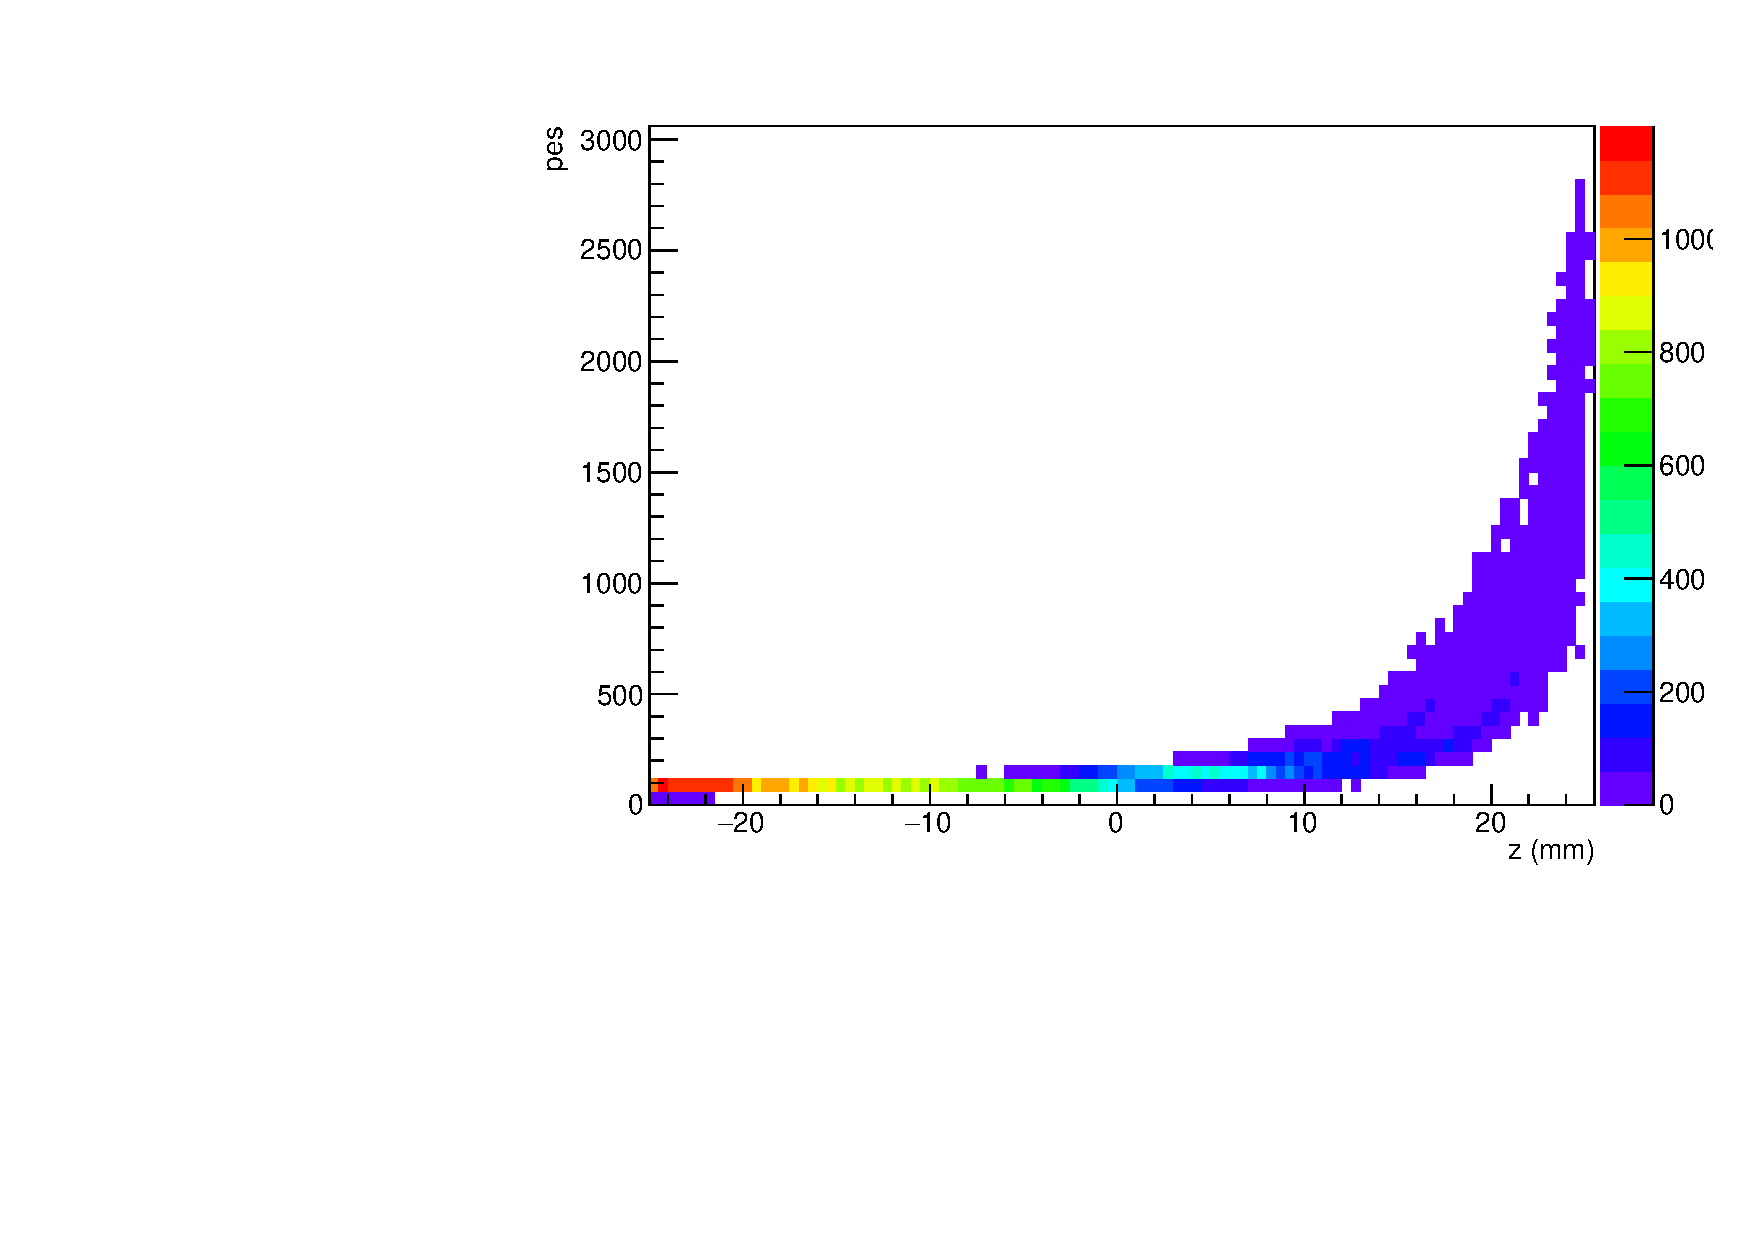
\includegraphics[width=.5\textwidth]{img/sipmmc_p2_2_z5.pdf}
		\label{fig.simpmmc_p2}
	}
	\caption{\label{fig.sipmm} (a) Number of photoelectrons in the SiPM registering the maximum signal as function of the distance to the entry plane ($z=-25$). (b) Number of photoelectrons in the SiPM registering the maximum signal as a function of the distance to the exit plane ($z=25$).}
\end{figure}

%LXSC6_64
\begin{figure}[!htb]
	\centering
	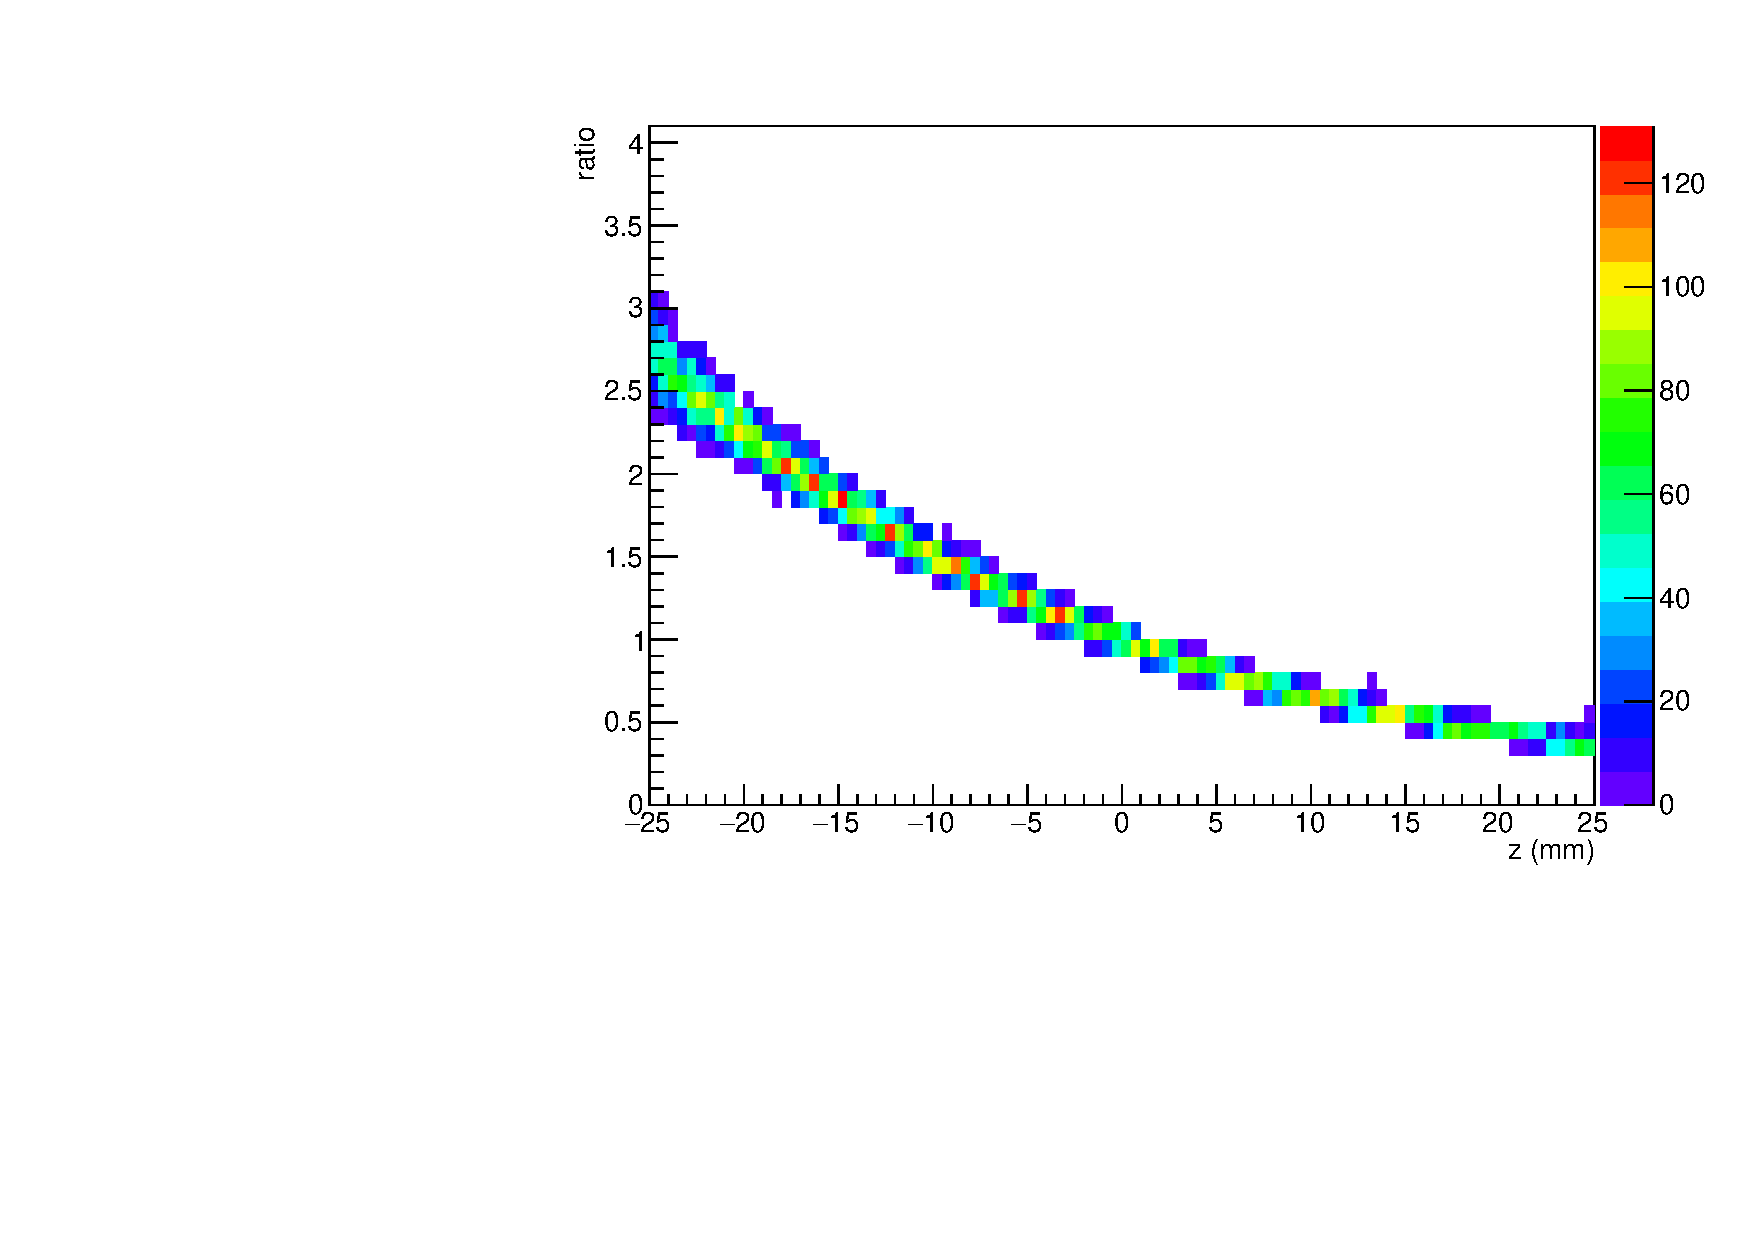
\includegraphics[scale=0.5]{img/zratio.pdf}
	\caption{\label{fig.zratio}  Ratio of the signal in the entry and the exit face (the signal in a face is defined as the sum of the signals of all its SiPMs) as a function of the longitudinal coordinate.}
\end{figure}

There is also some diffuse light that introduces noise in the detector, so if we want to compute barycenter properly, we need to apply some cuts. There are several approaches, we have tried two of them: (a) find the maximum SiPM in the plane and take only those SiPM having more than a percentage of its charge or (b) find the maximum SiPM and take those adjacent to it, build a cluster with the maximum on its center. The first approach has worked better for us, usually with a cut around 75\%.


\begin{table}[h]
\caption{\label{tab.position} Resolution (mm) in $x$ and $y$ coordinates for different LXSC configurations.}
\begin{center}
 \begin{tabular}{c|cc|cc|cc}
  \toprule
\multirow{2}{*}{Planes\textbackslash SiPM}  & \multicolumn{2}{c}{\textbf{36 SiPM}} & \multicolumn{2}{c}{\textbf{49 SiPM}} & \multicolumn{2}{c}{\textbf{64 SiPM}} \\
  \cline{2-7}
  & \textbf{x} & \textbf{y} & \textbf{x} & \textbf{y} & \textbf{x} & \textbf{y} \\
  \hline
    \textbf{2 Planes} & 2.1 & 2.1 & 1.8 & 1.8 & 1.9 & 1.9 \\
    \textbf{4 Planes} & 1.5 & 1.5 & 1.3 & 1.3 & 1.3 & 1.3 \\
    \textbf{6 Planes} & 0.9 & 0.9 & 0.8 & 0.7 & 0.8 & 0.8 \\
    \toprule
 \end{tabular}
\end{center}
\end{table}

\begin{table}[h]
\caption{\label{tab.positionZ} Resolution (mm) in $z$ coordinate for different LXSC configurations using the ratio entry/exit plane and using barycenter.}
\begin{center}
 \begin{tabular}{c|ccc}
  \toprule
  Planes\textbackslash SiPM & \textbf{36 SiPM} & \textbf{49 SiPM} & \textbf{64 SiPM} \\
   \hline
  \textbf{2 Planes (ratio)} & 1.5 & 1.3 & 1.2 \\
  \textbf{4 Planes (barycenter)} & 1.5 & 1.4 & 1.4 \\
  \textbf{6 Planes (barycenter)} & 0.9 & 0.8 & 0.9 \\
  \textbf{6 Planes (ratio)} & 1.2 & 1.0 & 1.0 \\
    \toprule
 \end{tabular}
\end{center}
\end{table}

\begin{figure}[!htb]
	\centering
	\subfloat[LXSC6\_64]{
		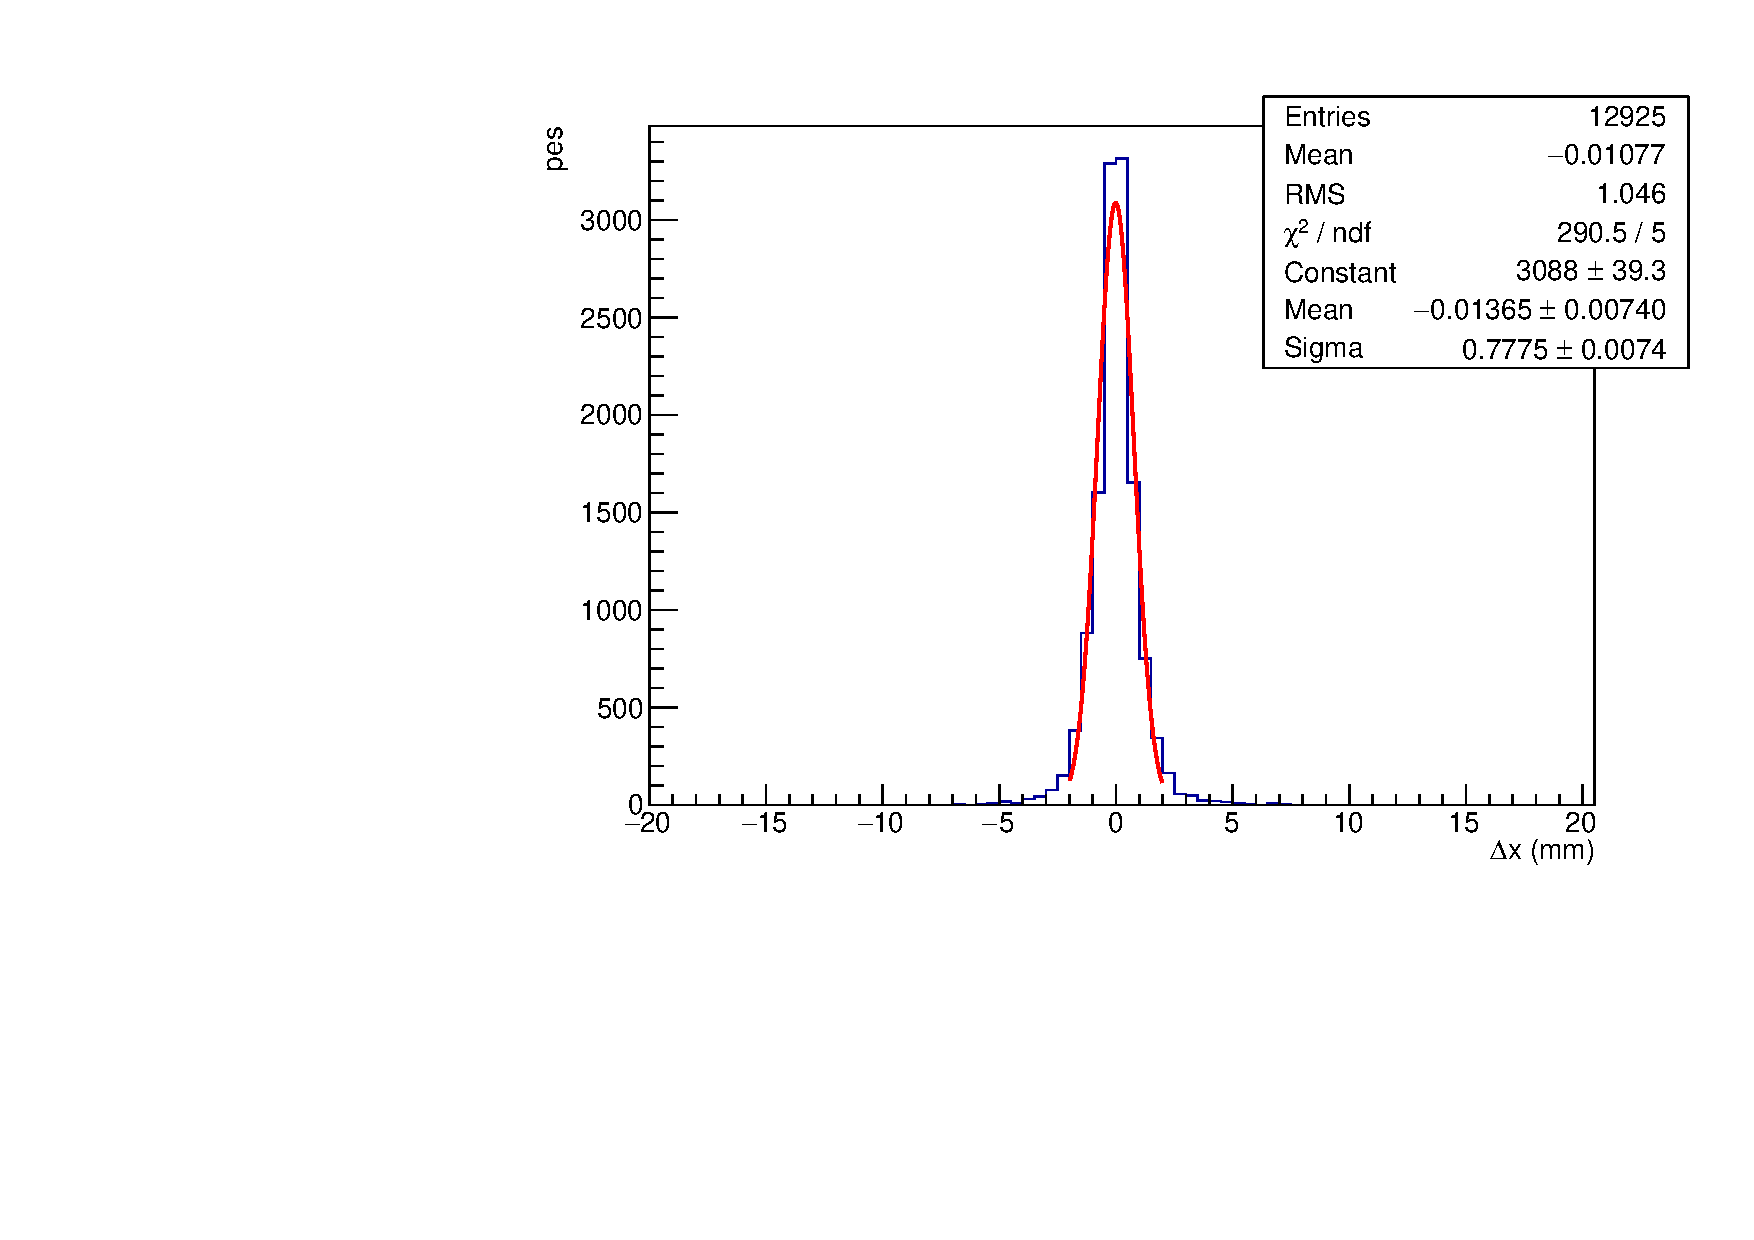
\includegraphics[width=.5\textwidth]{img/xBest_6_64.pdf}
	}
	\subfloat[LXSC2\_36]{
		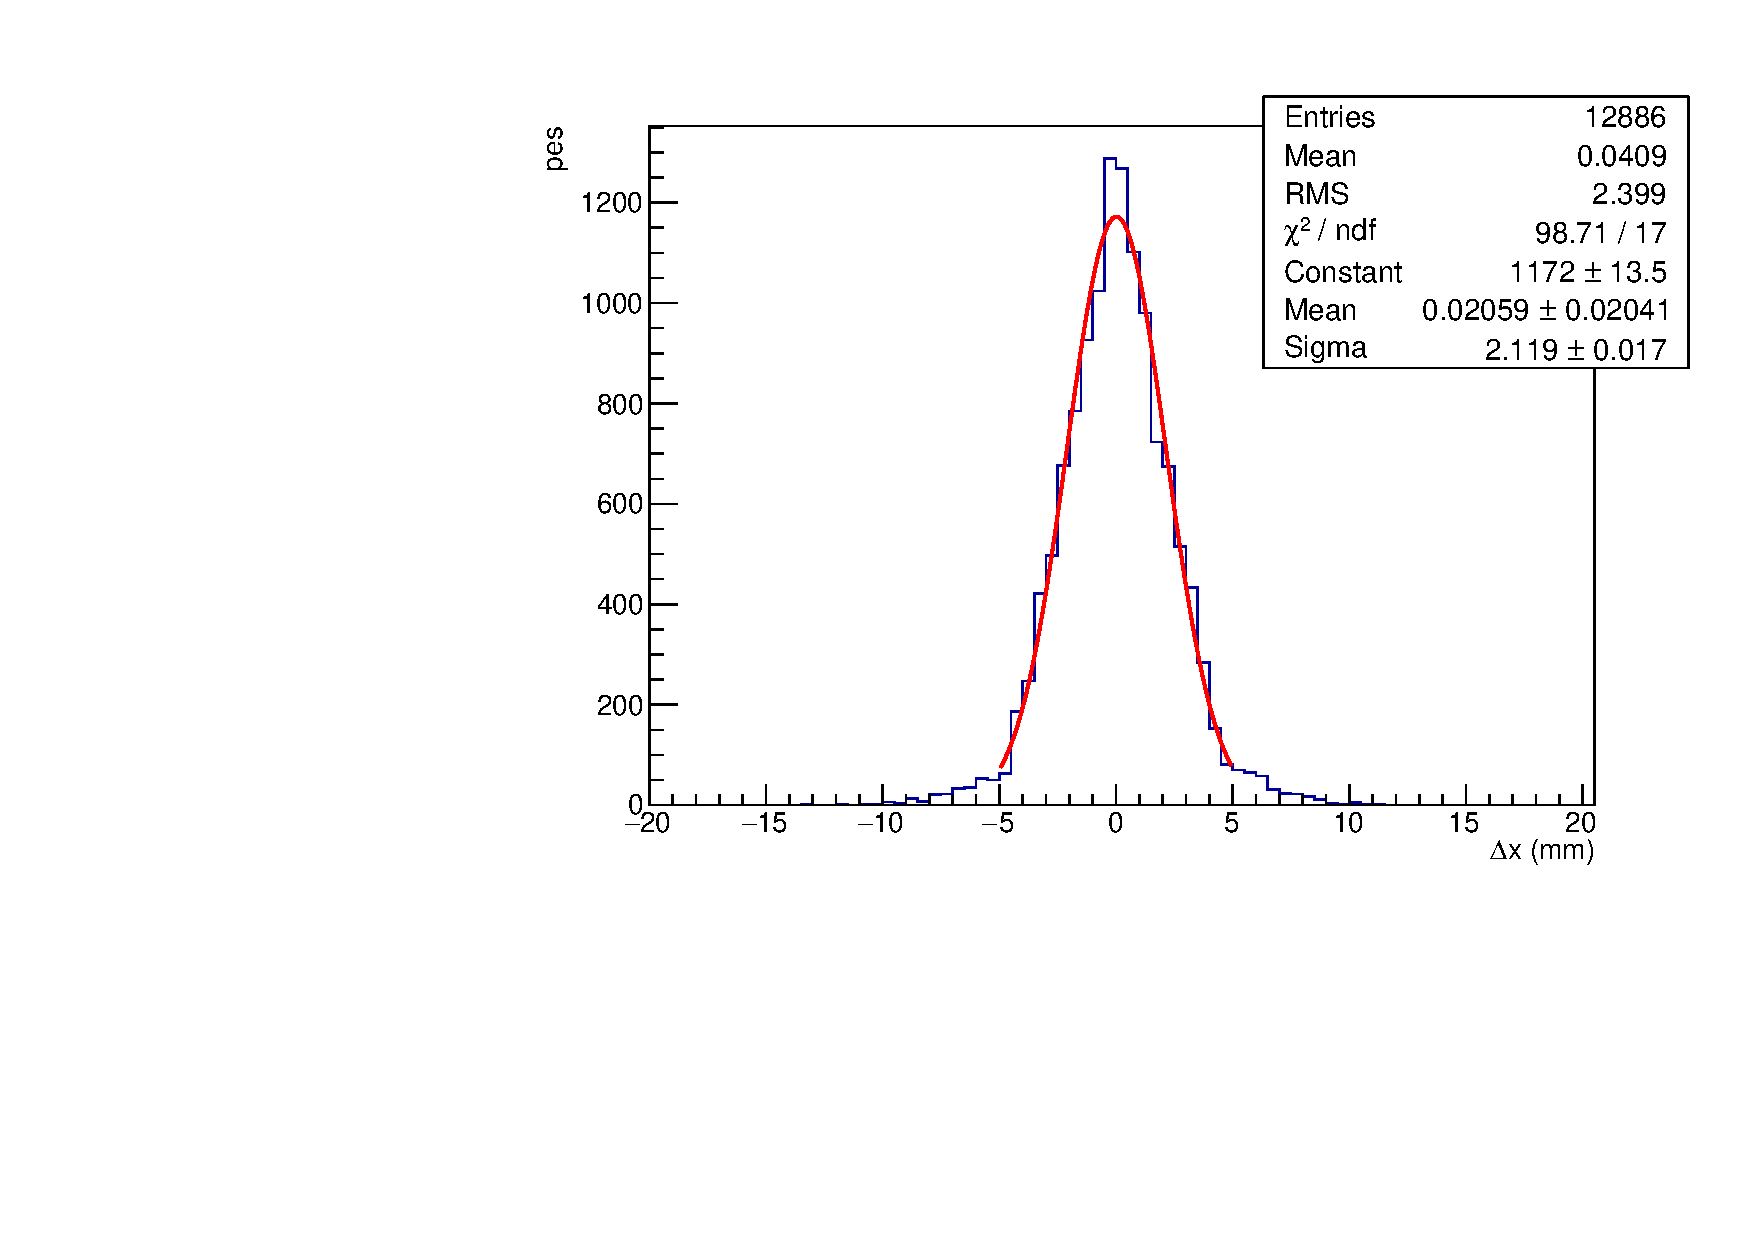
\includegraphics[width=.5\textwidth]{img/xBest_2_36.pdf}
	}
	\caption{\label{fig.xBest} Resolution in a transverse coordinate. (a) Best case, LXSC fully instrumented (6 planes with 64 SiPM each). (b) Worst case, most sparse configuration, 2 planes with 36 SiPM each.}
\end{figure}

%The resolution achieved with a box of $10\times10\times10$ cm$^3$ fully instrumented (LXSC10) is around 2.2 mm in the three coordinates. 

Table \ref{tab.position} shows the results for both transverse coordinates for different $5\times5\times5$ cm$^3$ configurations. Figure \ref{fig.xBest} show the histograms for best (LXSC6-64) and worst case (LXSC2-36).

In Table \ref{tab.positionZ} are shown the results for the longitudinal coordinate computed using barycenter or entry/exit ratio, it can be seen that the ratio works very well. 

As expected, reducing the amount of instrumentation leads to worse resolutions but the effect is quite mild, and appears as a good tradeoff for large PET scanners.  

Table \ref{tab.position2Z} shows how resolution changes if we reduce the longitudinal size of LXSC2. The transverse resolution improves by a factor of 2 for the thinner cell, while the longitudinal resolution worsens by a factor 40\%. However, the resolution in $z$~is still much better than the resolution that can be achieved by SSDs (the thickness of the detector over $\sqrt{12}$, typically $2/\sqrt{12} \sim 6 mm$~even for the thinner cell, and the improvement in transverse resolution may be relevant for small animal or brain PET. 

% It gets better but, as we have seen in previous sections, energy resolution is worse (see Table \ref{tab.energy2}) and, most important, many gammas cross the detector without interaction (see Table \ref{tab.lxscZ}). Therefore, we conclude that $5\times5\times5$ cm$^3$ is a good size for LXSC. The amount of instrumentation will ultimately be determined by the cost.
%
%We have also studied whether geometrical corrections are needed or not. Figure \ref{fig.bias} shows that near the edges (near the SiPMs) the reconstruction is better than in the middle, where the interaction point is far from both planes, but there is no bias we can correct geometrically.

\begin{table}[h]
\caption{\label{tab.position2Z} Resolution in the three coordinates for LXSC2 varying the longitudinal size.}
\begin{center}
 \begin{tabular}{c|ccc}
  \toprule
   {\bf Longitudinal size} & \textbf{$x$ coordinate} & \textbf{$y$ coordinate} & \textbf{$z$ coordinate}\\
   \hline
  {\bf 2 cm} & 1.0 & 1.0 & 1.8\\
  {\bf 3 cm} & 1.4 & 1.4 & 1.4\\
  {\bf 4 cm} & 1.7 & 1.7 & 1.4\\
  {\bf 5 cm} & 1.9 & 1.9 & 1.3\\
  \toprule
 \end{tabular}
\end{center}
\end{table}

%\begin{figure}[h]
%	\centering
%	\subfloat[$x$ coordinate]{
%		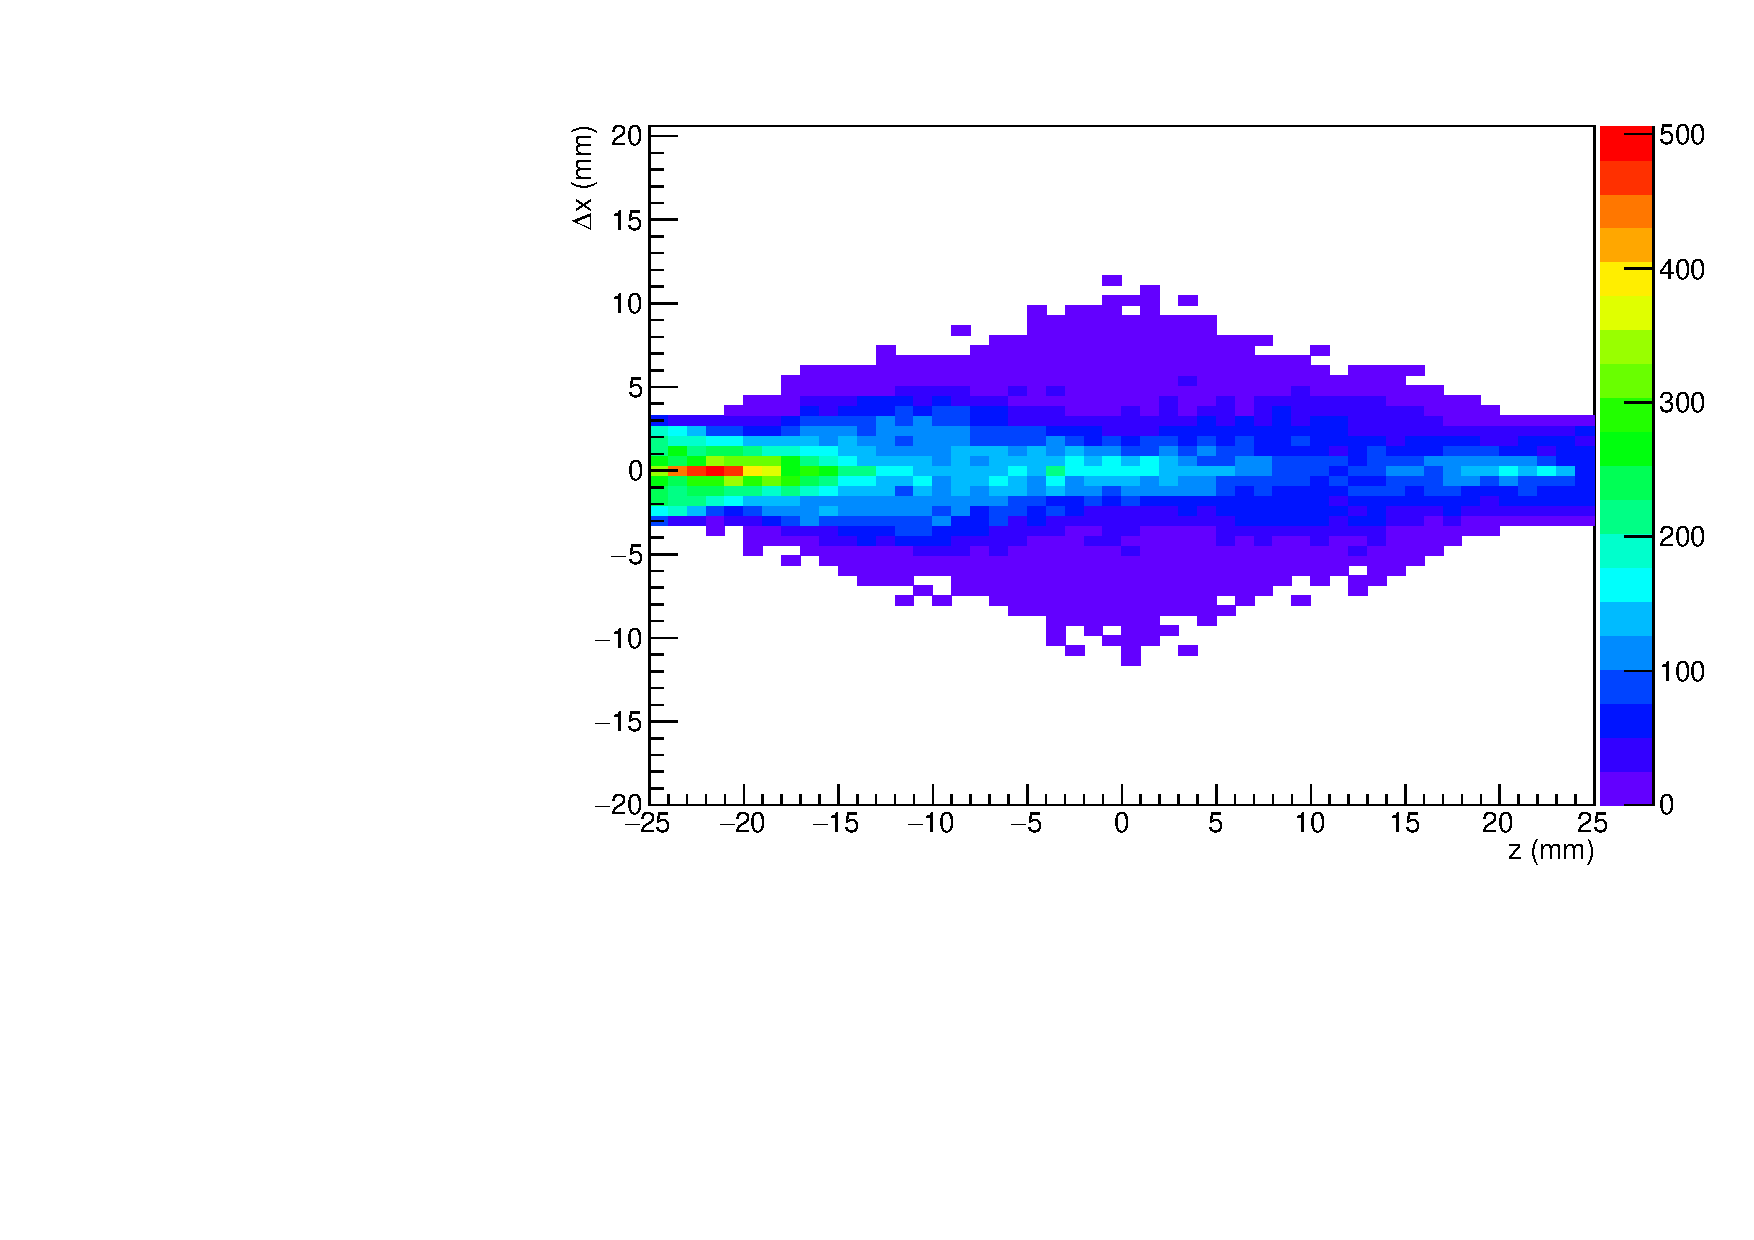
\includegraphics[width=.5\textwidth]{img/xbias.pdf}
%	}
%	\subfloat[$y$ coordinate]{
%		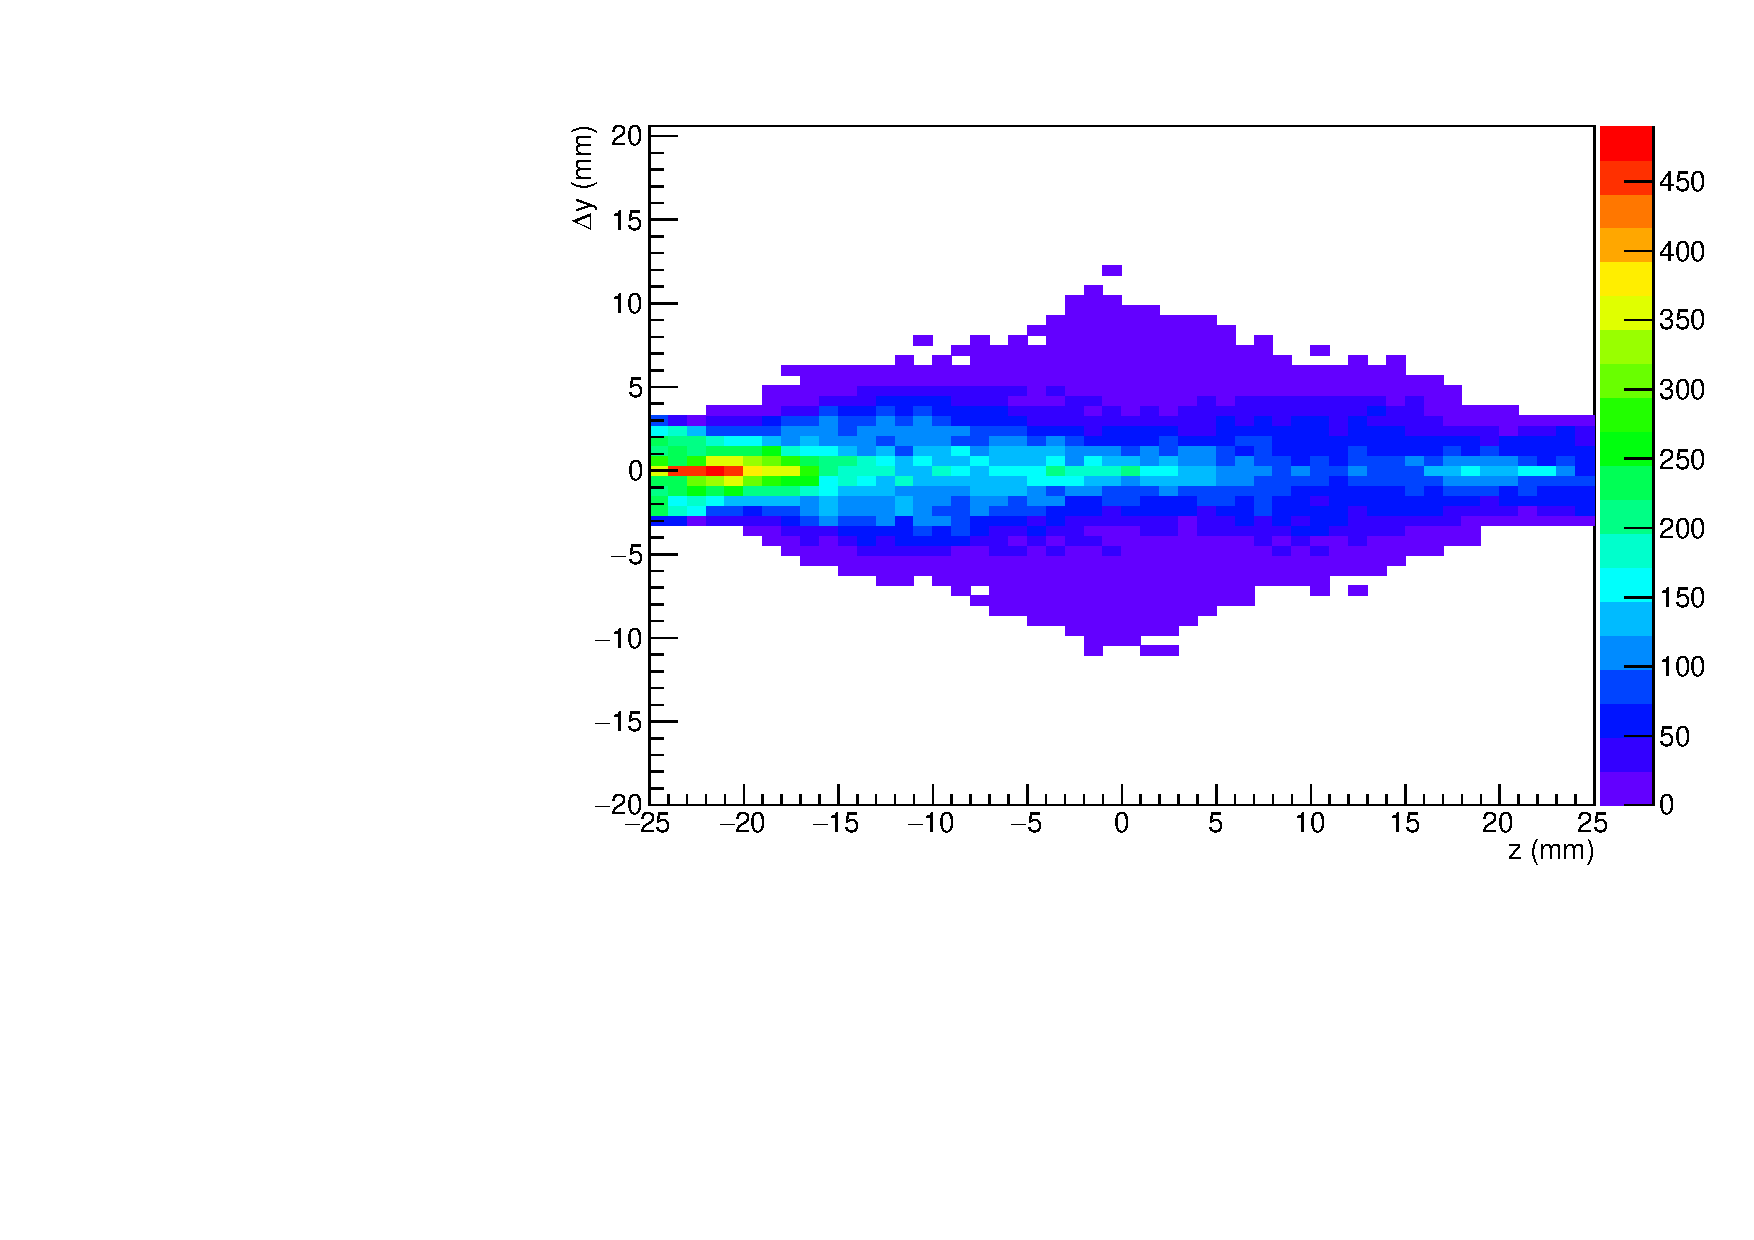
\includegraphics[width=.5\textwidth]{img/ybias.pdf}
%	}
%	\caption{\label{fig.bias} Difference between reconstructed position and true position for both transverse coordinates as a function of the longitudinal one.}
%\end{figure}

Summarizing, for the standard box dimensions, the space resolution obtained for the LXSC6 is better than 1 mm r.m.s. The resolution in the LXSC2 is better than 2 mm r.m.s. in the transverse coordinates ($x,y$) and 1.5 mm in the longitudinal coordinate. The transverse resolution can be improved by a substantial factor of 2 by reducing the thickness of the box to 2 cm. 

\subsection{Neural network}
Machine learning can also be used to reconstruct event positions. We have explored this possibility using neural networks, which is a set of connected nodes called {\it neurons}. Each one of them receives some numerical inputs, $x_i$, that have a weight associated, $w_i$. With this data the activation function is computed giving the output for one node: $y = f(\sum_i w_i x_i )$. We have used a common activation function, the logistic function: $f(x) = e^x/(1+e^x)$. The idea is illustrated on Figure \ref{fig.nnNode}. 

\begin{figure}[!h]
	\centering
\begin{tikzpicture}[
init/.style={
  draw,
  circle,
  inner sep=2pt,
  font=\Huge,
  join = by -latex
},
squa/.style={
  draw,
  inner sep=2pt,
  font=\Large,
  join = by -latex
},
start chain=2,node distance=13mm
]
\node[on chain=2] 
  (x2) {$x_2$};
\node[on chain=2,join=by o-latex] 
  {$w_2$};
\node[on chain=2,init] (sigma) 
  {$\displaystyle\Sigma$};
\node[on chain=2,squa,label=above:{\parbox{2cm}{\centering Activate \\ function}}]   
  {$f$};
\node[on chain=2,label=above:Output,join=by -latex] 
  {$y$};
\begin{scope}[start chain=1]
\node[on chain=1] at (0,1.5cm) 
  (x1) {$x_1$};
\node[on chain=1,join=by o-latex] 
  (w1) {$w_1$};
\end{scope}
\begin{scope}[start chain=3]
\node[on chain=3] at (0,-1.5cm) 
  (x3) {$x_3$};
\node[on chain=3,label=below:Weights,join=by o-latex] 
  (w3) {$w_3$};
\end{scope}
\node[label=above:\parbox{2cm}{\centering Bias \\ $b$}] at (sigma|-w1) (b) {};

\draw[-latex] (w1) -- (sigma);
\draw[-latex] (w3) -- (sigma);
\draw[o-latex] (b) -- (sigma);

\draw[decorate,decoration={brace,mirror}] (x1.north west) -- node[left=10pt] {Inputs} (x3.south west);
\end{tikzpicture}
	\caption{\label{fig.nnNode} Node of neural network.}
\end{figure}


The basic architecture of a feed-forward neural network is illustrated in Figure \ref{fig.nn}. There is one input layer with as many nodes as inputs there are to the problem, one or more hidden layers, each one with a number of hidden nodes and, finally, at the end, the output(s). All nodes in one layer are connected to those of the next layer. The input nodes only pass the values $x_i$ to the first hidden layer, each hidden node will compute its activation function $f_h$ and then pass the result to next level until the output(s) node(s), which will compute the final answer. Each connection between nodes will have a weight, which initially will be a random value. Therefore the output for a network with only one hidden layer will be:

$$ y = f_o \left(b_k + \sum_h w_{hk} f_h \left(b_h + \sum_i w_{ih}x_i\right) \right)$$
%
where $f_o$ is the output activation function, $w_{ij}$ are the weights from layer $i$ to layer $j$ and $b_j$ are {\it biases}, numbers that are added by each node to improve learning process.


\begin{figure}[!htb]
	\centering
	\begin{tikzpicture}[
	plain/.style={
	  draw=none,
	  fill=none,
	  },
	net/.style={
	  matrix of nodes,
	  nodes={
	    draw,
	    circle,
	    inner sep=10pt
	    },
	  nodes in empty cells,
	  column sep=2cm,
	  row sep=-9pt
	  },
	>=latex
	]
	\matrix[net] (mat)
	{
	|[plain]| \parbox{1.3cm}{\centering Input\\layer} & |[plain]| \parbox{1.3cm}{\centering Hidden\\layer} & |[plain]| \parbox{1.3cm}{\centering Output\\layer} \\
	& |[plain]| \\
	|[plain]| & \\
	& |[plain]| \\
	|[plain]| & |[plain]| \\
	& & \\
	|[plain]| & |[plain]| \\
	& |[plain]| \\
	|[plain]| & \\
	& |[plain]| \\
	};
	\foreach \ai [count=\mi ]in {2,4,...,10}
	  \draw[<-] (mat-\ai-1) -- node[above] {Input \mi} +(-2cm,0);
	\foreach \ai in {2,4,...,10}
	{\foreach \aii in {3,6,9}
	  \draw[->] (mat-\ai-1) -- (mat-\aii-2);
	}
	\foreach \ai in {3,6,9}
	  \draw[->] (mat-\ai-2) -- (mat-6-3);
	\draw[->] (mat-6-3) -- node[above] {Ouput} +(2cm,0);
	\end{tikzpicture}
	\caption{\label{fig.nn} Example Neural Network. All inputs are connected to all nodes in next layer (the hidden layer) and the hidden layer is connected to the output. We have use only only one hidden layer and one output.}
\end{figure}

This kind of techniques requires some {\it training}, we need a set of inputs for which we know the correct output to adjust the parameters of the network. The way this is done is using the backpropagation algorithm, which computes the output of the network
and make small corrections to the weights to minimize the error. This is repeated for all inputs in the training set, one iteration over all inputs is called an {\it epoch}. The algorithm stops when the error is less than a threshold  or when a maximum number of epochs is achieved. To measure the error the easiest way is using least-squares method.

We have tested this approach to reconstruct both transverse coordinates ($x$ and $y$) using as inputs all the SiPM values from the entry plane of a LXSC2 simulation. To do this we have trained two networks, one for each coordinate. The architecture chosen has 64 inputs nodes, one hidden layer with 100 nodes and one output. We have a dataset with 12925 photoelectric events and we divided it between 6463 for training set and 6462 for test set. After training the network we have compute the resolution for both sets. 

Results seem very promising as is shown by Figure \ref{fig.nnPlot}. There seems to be a little overfitting, but a good result overall. The histogram for test set is not completely gaussian but the majority of events has been well reconstructed. For $y$ coordinate we get similar results, having obtained resolutions of 0.652 and 1.051 mm for train and test respectively. Clearly, neural networks, and machine learning in a broader sense, seems like a very promising direction to further explore in this problem.


\begin{figure}[!htb]
	\centering
	\subfloat[Train set]{
		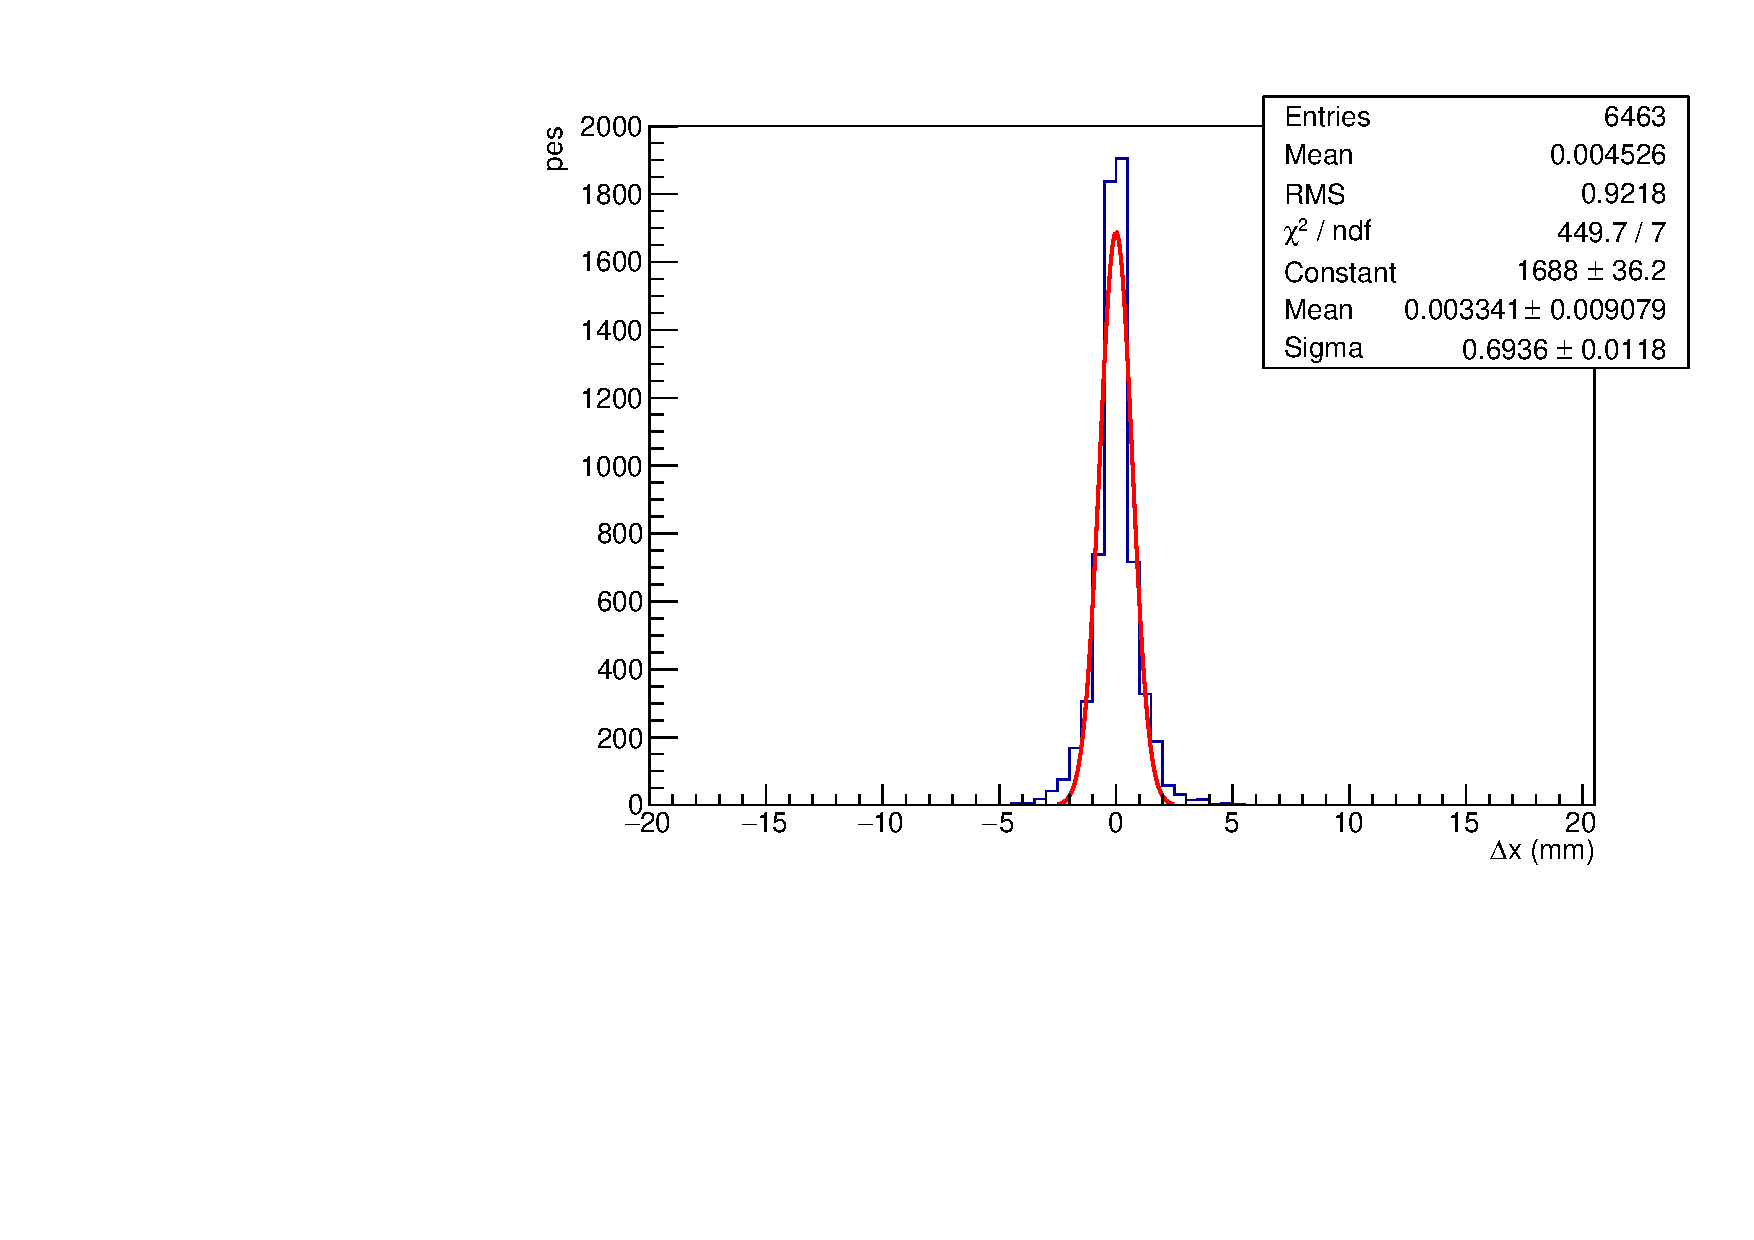
\includegraphics[width=.5\textwidth]{img/nn_trainX.pdf}
		\label{fig.nnPlotTrain}
	}
	\subfloat[Test set]{
		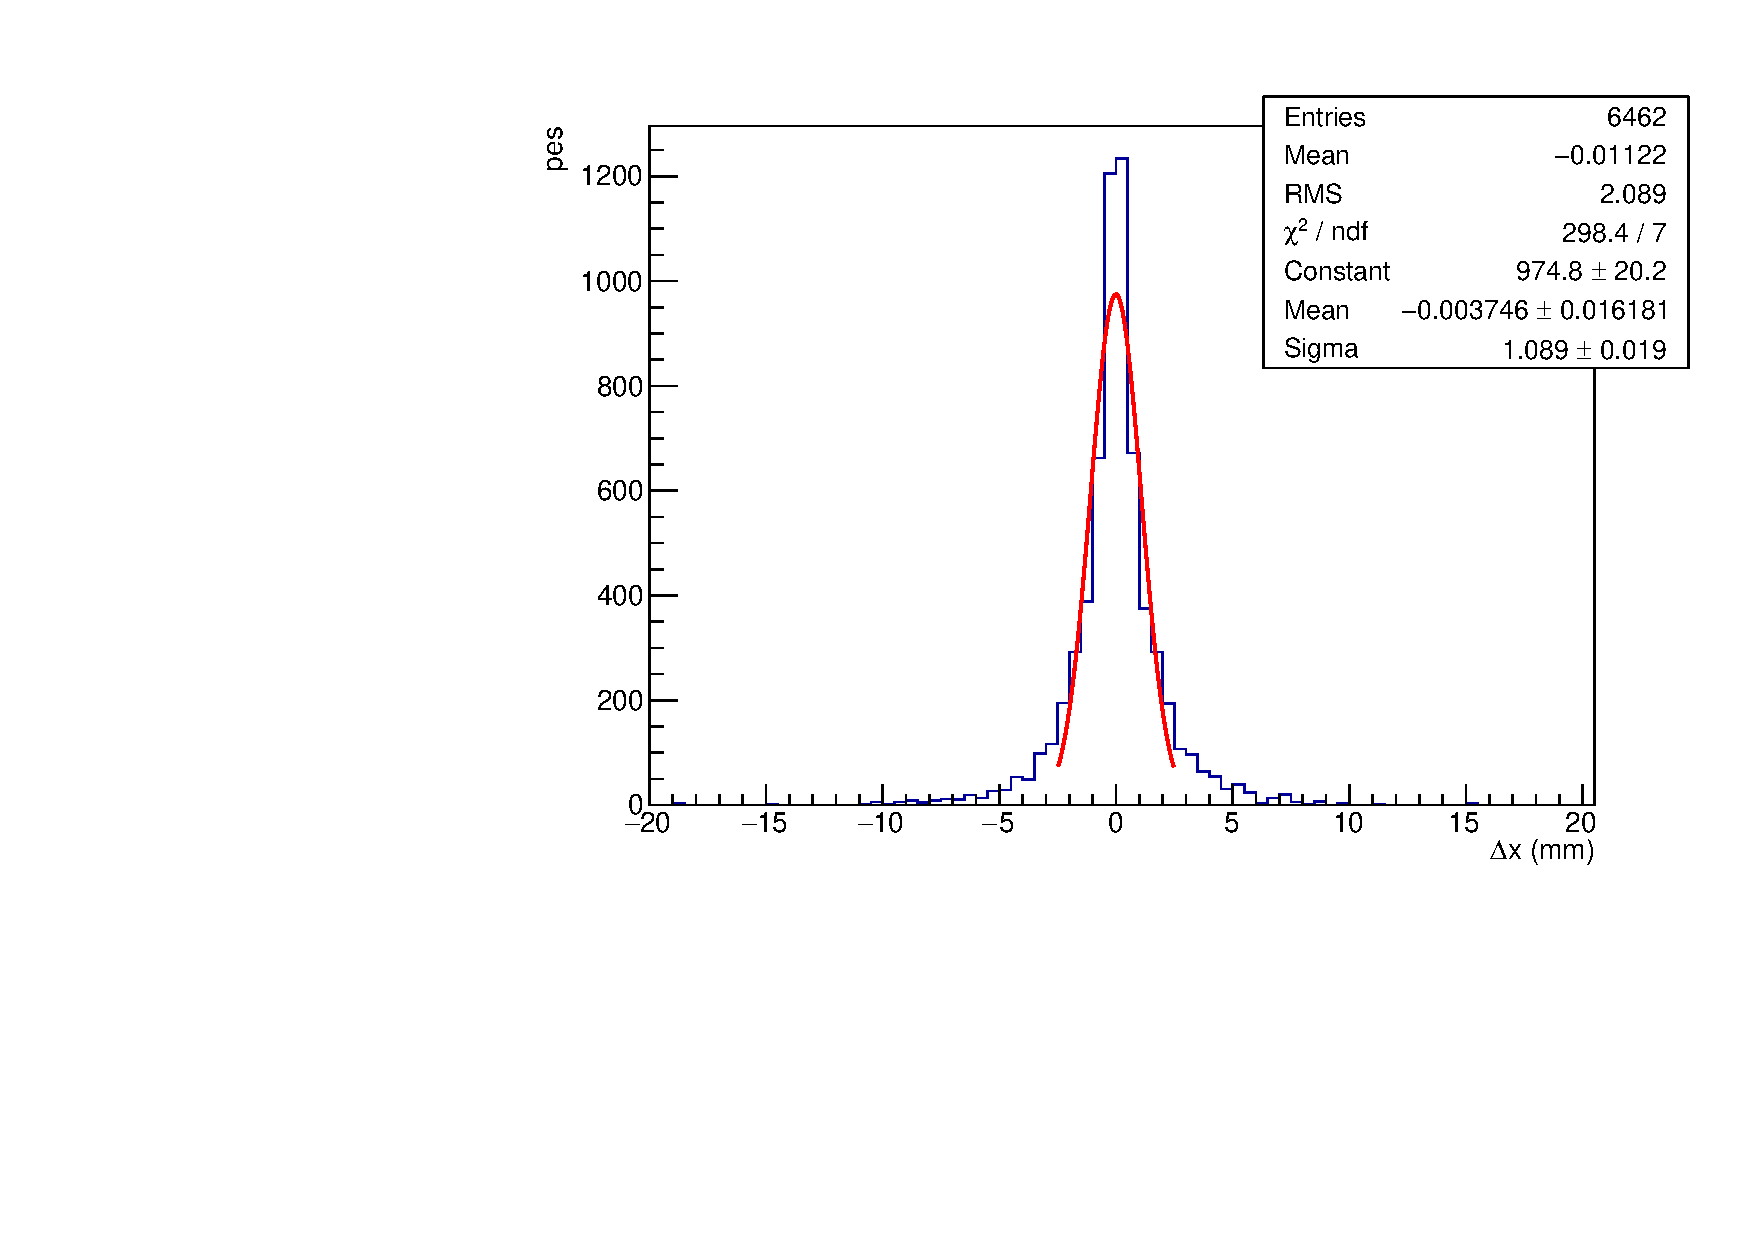
\includegraphics[width=.5\textwidth]{img/nn_testX.pdf}
		\label{fig.nnPlotTest}
	}
	\caption{\label{fig.nnPlot} Resolution in $x$ coordinate using a neural network to reconstruct position. (a) Resolution for train set. (b) Resolution for test set.}
\end{figure}

